%# -*- coding:utf-8 -*-
%=========================================================================%
%   LaTeX File for phd thesis of Institute of Automation, CAS
%-------------------------------------------------------------------------%
%
%   revised by Fan Yang (fan.yang@ia.ac.cn) at Jan, 2013
%
%   * 修正了参考文献书签定位不准的问题
%   * 修正了书签的层次结构
%   * 为中英文封面和摘要生成书签
%
%-------------------------------------------------------------------------%
%
%   revised by Jian Cheng (jian.cheng.1983@gmail.com) at November, 2011
%
%   * utf8编码,可以工作在texlive in linux 或者 ctex in windows
%   * 生成可以拷贝的中文
%   * 用utf8解决中文书签乱码的问题
%
%-------------------------------------------------------------------------%
%   Revised by Zhaoxiang Zhang (zxzhang@nlpr.ia.ac.cn) at April, 2007
%
%   本模板要求满足GPL协议,可以自行修改并发布,但必须公布代码
%
%-------------------------------------------------------------------------%
%   Revised by J. G. Lou (jglou@nlpr.ia.ac.cn) at April, 2003
%-------------------------------------------------------------------------%
%   Latex 博士论文模板.
%   建议使用miktex2.1最大安装编译此模板
%   本模板使用ctex.org的cjk版本 和aloft 修改后的gb_aloft.cap,
%   如果安装的是miktex包自带的cjk 请用srcbook 替换 book
%=========================================================================%
%%%%%%%%%%%%%%%%%%%%%%%%%%%%%%%%%%%%%%%%%%%%%%%%%%%%%%%%%%%%%%%
%文件头部定义
%%%%%%%%%%%%%%%%%%%%%%%%%%%%%
\documentclass [12pt,a4paper,twoside] {book}
%\documentclass [12pt,a4paper,openany,twoside,draft] {book}
%============================ 引用的宏包 ==================================%
%# -*- coding:utf-8 -*-
%=========================================================================%
%   LaTeX File for phd thesis of Institute of Automation, CAS
%-------------------------------------------------------------------------%
%   张兆翔将原来的dvipdf改为dvipdfm宏包,可使用latex + dvipdf自动生成索引
%-------------------------------------------------------------------------%
%   Revised by J. G. Lou (jglou@nlpr.ia.ac.cn)
%-------------------------------------------------------------------------%
%=========================================================================%
%                          引用的宏包和相应的定义
%=========================================================================%

%============================ 中文支持宏包 ==============================%
% \usepackage{CJK}
\usepackage{CJKutf8}

%====================== 图形和超链接支持宏包 ========================%
% 图形支持宏包 为了使用PDFLaTeX需要作相应判断
% hyperref
% 可以在转换为pdf文件时自动加入索引, dvi2ps 加入-z 参数
% 为了支持pdftex 使用不同的宏包选项
\ifx\pdfoutput\undefined
\usepackage[dvips]{graphicx}
\usepackage[dvipdfm,
            pagebackref,
            %backref,
            unicode=true,
            % CJKbookmarks=true,
            bookmarksnumbered=true
            % bookmarksopen=false,
            ]{hyperref}
\else
\usepackage[dvipdfm,
            pagebackref,
            %backref,
            unicode=true,
            % CJKbookmarks=true,
            bookmarksnumbered=true
            ]{hyperref}
\usepackage[pdftex]{graphicx}
\fi


% \usepackage{ccmap}


\usepackage{color}      % 支持彩色
\usepackage{subfigure}  % 支持子图
\usepackage{floatflt}   % 图文混排用宏包
\usepackage{rotating}   % 图形和表格的控制
\usepackage{flafter}    % 因为图形可浮动到当前页的顶部,所以它可能会出现
                        % 在它所在文本的前面. 要防止这种情况,可使用 flafter
                        % 宏包

\usepackage[below]{placeins}    %浮动图形控制宏包
                                %允许上一个section的浮动图形出现在下一个
                                %section的开始部分该宏包提供处理浮动对象
                                %的 \FloatBarrier 命令,使所有未处理的浮动
                                %图形立即被处理
%\usepackage{endfloat}  %可将浮动对象放置到文件的最后
%\usepackage{overpic}   %将LaTeX对象放置在图上
%\usepackage{pstricks}  %Postscript macrosfor Generic TeX(我没用过,据说很强)
\usepackage{bez123}

%============================表格支持宏包=================================%
\usepackage{rotating}   % 用法 \begin{sidewaystable}....\end{sidewaystable}
                        % 即可旋转表格
\usepackage{longtable}  % 支持长表格
\usepackage{tabls}
\usepackage{multirow}   % 表格多行合并, 矩阵的边注
\usepackage{colortbl}   % 彩色表格
\usepackage{dcolumn}    % 让表格中将小数点对齐
\usepackage{hhline}     % 在表格中用 \hhline 得到的结果就如同\hline
                        % 或 \hline\hline,当然在和垂直线的交叉处会有所不同。
\usepackage{slashbox}   % 可在表格的单元格中画上一斜线。

%\newcommand{\centpcol}{\leftskip\fill \rightskip\fill}%制表使可用p{ncm}设置栏宽,还使本栏居中

%\iffalse 举例
%  \begin{tabular}{|l|c|c|} \hline
%    & \multicolumn{2}{c|}{MRD} \\ \cline{2-3}
%   & \multicolumn{1}{p{3.5cm}|}{\centpcol Same as previous response} &
%     \multicolumn{1}{p{3.5cm}|}{\centpcol Different from previous response}\\
%   \hline
%    Observed frequency & 966 & 148 \\
%    Expected frequency & 1066 & 48 \\ \hline
%    \multicolumn{3}{c}{${\chi}^2 = 213.97,\quad \mathit{d.f.}=1,\quad p<0.001$}
%  \end{tabular}
%\fi

%============================版面控制宏包=================================%
\usepackage[top=3.0cm,bottom=3.3cm,left=3.2cm,right=3.2cm, headheight=0.5cm, headsep=1.0cm, footskip=1.5cm %,includehead,includefoot
            ]{geometry}                 % 页面设置
\usepackage{indentfirst}                % 首行缩进宏包
\usepackage[perpage,symbol]{footmisc}   % 脚注控制
\usepackage{fancyhdr}                   % fancyhdr宏包 页眉和页脚的相关定义
\usepackage{lastpage}                   %自动记录总页数宏包,计数器为 LastPage
                                        %注意大小写
\usepackage{pageno}     % 章首页的页眉处理, 可以改为自己想要的形式
%\iffalse \makeatletter
%\renewcommand{\ps@plain}{%
%   \renewcommand{\@mkboth}{\@gobbletwo}%
%   \renewcommand{\@evenhead}{\reset@font\sf -- \thepage -- \hfil}%
%   \renewcommand{\@oddhead}{\reset@font\sf\hfil -- \thepage --}%
%   \renewcommand{\@evenfoot}{}%
%   \renewcommand{\@oddfoot}{}
%} \makeatother \fi

%======================= 多列文本与多列编号宏包 ===========================%
\usepackage{multicol,multienum}
%\iffalse 用法为:可嵌套使用
%\begin{multienumerate}[evenlist,oddlist]
%\mitemxxxx{Not}{Linear}{Not}{Quadratic}
%\mitemxxxo{Not}{Linear}{No; if $x=3$, then $y=-2$.}
%\mitemxx{$(x_1,x_2)=(2+\frac{1}{3}t,t)$ or
%$(s,3s-6)$}{$(x_1,x_2,x_3)=(2+\frac{5}{2}s-3t,s,t)$}
%\end{multienumerate}
%\begin{multicols}{2}
%\end{multicols}
%\fi

%======================== 数学公式相关宏包 ===============================%
\usepackage{bm}         % 处理数学公式中的黑斜体的宏包
\usepackage{amsmath}    % AMSLaTeX宏包 用来排出更加漂亮的公式
\usepackage{amssymb}    % AMSLaTeX宏包 用来排出更加漂亮的公式
\usepackage{mathrsfs}  % 不同于\mathcal or \mathfrak 之类的英文花体字体
\usepackage[amsmath,thmmarks]{ntheorem} % 定理类环境宏包,其中 amsmath 选项
                                        % 用来兼容 AMS LaTeX 的宏包
\usepackage{subeqnarray} %多个子方程(1-1a)(1-1b)
%\iffalse 以下是一个例子
%\begin{subeqnarray}
%\label{eqw} \slabel{eq0}
% x & = & a \times b \\
%\slabel{eq1}
% & = & z + t\\
%\slabel{eq2}
% & = & z + t
%\end{subeqnarray}
%\fi

%=============================标题与列表宏包=============================%
\usepackage[sf]{titlesec}   % 控制标题的宏包,配合命令在后面,
                            % 将cjk+miktex+scrbook+gb.cap下的章的标题号,
                            % 比如~``第二章 XXX''位置于中心
\usepackage{cite}           % 支持引用的宏包
\usepackage{enumerate}      % 改变列表标号样式宏包 其后可接选项[a,A,i,I,1]
\usepackage{caption2}       % 浮动图形和表格标题样式,可选项为
                            % [scriptsize,footnotesize,centerlast]
%\usepackage{setspace}      % 图形和表格的标题如果是多行,行距比较大,可以加宏包
\usepackage{pifont}         % 有很漂亮的带圈的各种数字符号使用
%\usepackage{atbeginend}    % 可选宏包, 能解决许多问题,
                            % 比如itemize, enumerate环境\item之间的控制
%用法
%\AfterBegin{itemize}{\addtolength{\itemsep}{-0.5\baselineskip}}
%\AfterBegin{enumerate}{\addtolength{\itemsep}{-0.5\baselineskip}}

%=================== 支持LaTexCAD生成的源程序的宏包 =====================%
\usepackage{TEXcad/lgrind}     % for formated source code
\usepackage{TEXcad/latexcad}   % latexcad.sty for drawings etc
\usepackage{TEXcad/epic}       %picture macros
\usepackage{TEXcad/eepic}      %extended picture macros
\usepackage{TEXcad/fancybox}   %box macros
\usepackage{TEXcad/epsf}       %postscript macros
\usepackage{TEXcad/rotate}     % postscript text rotation macros


%=========================== 特殊文本元素宏包 ==============================%
\usepackage{nicefrac}   % 在正文文本中排版分式时,可以用它来得到较好的排版效果。
\usepackage{units}      % 基于 nicefrac 宏包,提供对计量单位比较美观的排版效果。
\usepackage{soul}       % 支持对单词加上下划线或其每个字母在一定的宽度内均匀散布
\usepackage{altfont}    % 使用该宏包, 可以在一个宏包中使用多种不同的字体,
                        % 包括PSNFSS 和 MFNFSS
%\usepackage{prelim2e}  % 可以在每页页脚下方标记出本文档的版本信息等
\usepackage{a0size}     % 自由定义字号,在后面“字号设置”中可设置到107pt为止的大字体
%\usepackage{ulem}      % 用于支持文字内容的删除(非latex源文件中的注释!)(对中文的支持不够好,不会换行)
\usepackage{CJKulem}    % 用于支持文字内容的删除(非latex源文件中的注释!)(CJK字体专用)

\begin{document}
\begin{CJK*}{UTF8}{song}



\graphicspath{{figures/}}   %定义所有的eps文件在 image 子目录下

%=========================== 文本格式定义 =================================%
%# -*- coding:utf-8 -*- 
%=========================================================================%
%   LaTeX File for phd thesis of Institute of Automation, CAS
%-------------------------------------------------------------------------%
%   张兆翔重新修改了相关格式,以满足最新要求
%-------------------------------------------------------------------------%
%   Revised by J. G. Lou (jglou@nlpr.ia.ac.cn)
%-------------------------------------------------------------------------%

%=========================================================================%
%                          主文档 格式定义
%=========================================================================%

%===================== 重定义字体、字号命令 =============================%
% 注意win2000,没有 simsun, 最好到网上找一个。一些字体是office2000带的
\newcommand{\song}{\CJKfamily{song}}    % 宋体   (Windows自带simsun.ttf)
\newcommand{\fs}{\CJKfamily{fs}}        % 仿宋体 (Windows自带simfs.ttf)
\newcommand{\kai}{\CJKfamily{kai}}      % 楷体   (Windows自带simkai.ttf)
\newcommand{\hei}{\CJKfamily{hei}}      % 黑体   (Windows自带simhei.ttf)
\newcommand{\li}{\CJKfamily{li}}        % 隶书   (Windows自带simli.ttf)
\newcommand{\you}{\CJKfamily{you}}      % 幼圆   (Windows自带simyou.ttf)
\newcommand{\chuhao}{\fontsize{42pt}{\baselineskip}\selectfont}     % 字号设置
\newcommand{\xiaochuhao}{\fontsize{36pt}{\baselineskip}\selectfont} % 字号设置
\newcommand{\yihao}{\fontsize{28pt}{\baselineskip}\selectfont}      % 字号设置
\newcommand{\erhao}{\fontsize{21pt}{\baselineskip}\selectfont}      % 字号设置
\newcommand{\xiaoerhao}{\fontsize{18pt}{\baselineskip}\selectfont}  % 字号设置
\newcommand{\sanhao}{\fontsize{15.75pt}{\baselineskip}\selectfont}  % 字号设置
\newcommand{\sihao}{\fontsize{14pt}{\baselineskip}\selectfont}      % 字号设置
\newcommand{\xiaosihao}{\fontsize{12pt}{\baselineskip}\selectfont}  % 字号设置
\newcommand{\wuhao}{\fontsize{10.5pt}{\baselineskip}\selectfont}    % 字号设置
\newcommand{\xiaowuhao}{\fontsize{9pt}{\baselineskip}\selectfont}   % 字号设置
\newcommand{\liuhao}{\fontsize{7.875pt}{\baselineskip}\selectfont}  % 字号设置
\newcommand{\qihao}{\fontsize{5.25pt}{\baselineskip}\selectfont}    % 字号设置

%===================================================================%
%                         各种距离与缩进
%===================================================================%

%-------------------- 用于中文段落缩进 和正文版式 ------------------%
\CJKcaption{GB_aloft_UTF8}
\setlength{\parindent}{2em}                 % 首行两个汉字的缩进量
\setlength{\parskip}{3pt plus1pt minus1pt}  % 段落之间的竖直距离
\renewcommand{\baselinestretch}{1.2}        % 定义行距

%------------------------- 列表与图表距离设置 -----------------------%
\setlength{\topsep}{3pt plus1pt minus2pt}           % 第一个item和前面版落间的距离
\setlength{\partopsep}{3pt plus1pt minus2pt}        % 当在一个新页开始时加到
                                                    % \topsep的额外空间
\setlength{\itemsep}{3pt plus1pt minus2pt}          % 连续items之间的距离.
\setlength{\floatsep}{10pt plus 3pt minus 2pt}      % 图形之间或图形与正文之间的距离
\setlength{\abovecaptionskip}{2pt plus1pt minus1pt} % 图形中的图与标题之间的距离
\setlength{\belowcaptionskip}{3pt plus1pt minus2pt} % 表格中的表与标题之间的距离

%下面这组命令使浮动对象的缺省值稍微宽松一点,从而防止幅度
%对象占据过多的文本页面,也可以防止在很大空白的浮动页上放置
%很小的图形。
\renewcommand{\textfraction}{0.15}
\renewcommand{\topfraction}{0.85}
\renewcommand{\bottomfraction}{0.65}
\renewcommand{\floatpagefraction}{0.60}

%---------------------------- 数学公式设置 ------------------------------%
\setlength{\abovedisplayskip}{2pt plus1pt minus1pt}     %公式前的距离
\setlength{\belowdisplayskip}{2pt plus1pt minus1pt}     %公式后面的距离
\setlength{\arraycolsep}{2pt}   %在一个array中列之间的空白长度, 因为原来的太宽了

\allowdisplaybreaks[4]  % \eqnarray如果很长,影响分栏、换行和分页
                        %(整块挪动,造成页面空白),可以设置成为自动调整模式

%===================================================================%
%                         各种标题样式
%===================================================================%
%======================= 标题名称中文化 ============================%
\renewcommand\contentsname{目\ 录}
\renewcommand\listfigurename{插图目录}
\renewcommand\listtablename{表格目录}
%\renewcommand\abstractname{摘\ 要} %err undefined
%\renewcommand\refname{参考文献}         %article类型
\renewcommand\bibname{参\ 考\ 文\ 献}    %book类型
\renewcommand\indexname{索\ 引}
\renewcommand\figurename{图}
\renewcommand\tablename{表}
\renewcommand\partname{部分}


%======================= 定制章节的标题样式 =============================%
\setcounter{secnumdepth}{3}
%---------------------- 定义章节的编号格式 --------------------------%
%\renewcommand{\thesection}{\CJKnumber{\arabic{section}}、} % 定义 一、。九、十
\renewcommand{\thesection}{\arabic{chapter}.\arabic{section}}
\renewcommand{\thesubsection}{\arabic{chapter}.\arabic{section}.\arabic{subsection}}
\renewcommand{\thesubsubsection}{\arabic{chapter}.\arabic{section}.\arabic{subsection}.\arabic{subsubsection}}
\let\oldtitle=\title
\def\title#1{\oldtitle{\cnbf{#1}}}
\renewcommand{\CJKglue}{\hskip 0pt plus 0.08\baselineskip}

%----------------------- 定义章节标题格式 ----------------------------%
\titleformat{\chapter}[hang]{\fontsize{15pt}{15pt}\selectfont\filcenter\CJKfamily{hei}}
    {\fontsize{15pt}{15pt}\selectfont{\chaptertitlename}}{20pt}{\fontsize{15pt}{15pt}\selectfont}
\titlespacing{\chapter}{0pt}{-3ex  plus .1ex minus .2ex}{2.5ex plus .1ex minus .2ex}

%\titleformat{\section}[hang]{\CJKfamily{hei}\Large \centering} %标题居中
\titleformat{\section}[hang]{\CJKfamily{hei}\fontsize{14pt}{14pt}\selectfont}
    {\fontsize{14pt}{17pt}\selectfont \thesection}{1em}{}{}
\titlespacing{\section}
    {0pt}{1.5ex plus .1ex minus .2ex}{\wordsep}

\titleformat{\subsection}[hang]{\CJKfamily{hei}\fontsize{13pt}{13pt}\selectfont}
    { \fontsize{13pt}{13pt}\selectfont\thesubsection}{1em}{}{}
\titlespacing{\subsection}%
    {0pt}{1.5ex plus .1ex minus .2ex}{\wordsep}

\titleformat{\subsubsection}[hang]{\CJKfamily{hei}\fontsize{12pt}{12pt}\selectfont}
    {\fontsize{12pt}{12pt}\selectfont\thesubsubsection}{1em}{}{}
\titlespacing{\subsubsection}%
    {0pt}{1.2ex plus .1ex minus .2ex}{\wordsep}

%======================= 定义列表项目格式 ==========================%
\renewcommand\labelenumi{\textcircled{\scriptsize \theenumi}}  %带圈的数字
%\renewcommand\labelenumi{(\theenumi)}
\renewcommand\labelenumii{(\theenumii)}
\renewcommand\labelenumiii{\theenumiii.}
\renewcommand\labelenumiv{\theenumiv.}

%====================== 定制图形和表格标题样式 =====================%
%---------------------- 定制图形和表格标题格式 ---------------------%
\renewcommand{\captionlabeldelim}{}
\renewcommand{\captionlabelfont}{\small \CJKfamily{hei}\bf}
\renewcommand{\captionfont}{\small \CJKfamily{song}\rmfamily}
%% \scriptsize \footnotesize \small \large \Large  %图形标签字体大小

%--------------------- 定义图、表、公式的编号格式 -------------------%
\renewcommand{\thetable}{\arabic{chapter}-\arabic{table}}
\renewcommand{\theequation}{\arabic{chapter}-\arabic{equation}}
\renewcommand{\thefigure}{\arabic{chapter}-\arabic{figure}}


%=========================== 目录设置 ==================================%
\setcounter{tocdepth}{3} \setcounter{secnumdepth}{3}
% 可以用\section[abc]{abcdefg}形式的命令,这样abc就做为缩短标题出现
% 在目录表中和页眉上.另外,还可以利用\addtocounter{secnumdepth}{num}
% 来使得当前章节编号深度增加或减小,num可取正值或负值.

%============================= 页面设置 ================================%
%-------------------- 定义页眉和页脚 使用fancyhdr 宏包 -----------------%
\newcommand{\makeheadrule}{%
    %\makebox[0pt][l]{\rule[.7\baselineskip]{\textwidth}{1.2pt}}
    \rule[.6\baselineskip]{\linewidth}{0.4pt}\vskip-.8\baselineskip}
\makeatletter
\renewcommand{\headrule}{%
    {\if@fancyplain\let\headrulewidth\plainheadrulewidth\fi
     \makeheadrule }} %
\makeatother                                % 定义页眉与正文间隔线

\pagestyle{fancyplain}
\renewcommand{\chaptermark}[1]%
{\markboth{\chaptername \ #1}{}}            % 去掉章节标题中的数字
\fancyhf{} %\fancyfoot[C,C]{\thepage}

\fancyhead[CO]{\CJKfamily{fs}\leftmark}          % 在book文件类别下,
\fancyhead[CE]{\CJKfamily{fs}\rightmark}         % \leftmark自动存录各章之章名,

\fancyfoot[C]%                                  % [RE][LO]
{\CJKfamily{hei} -\;\thepage\;-}

%=== 配合前面的ntheorem宏包产生各种定理结构,重定义一些正文相关标题 ===%
\theoremstyle{plain}
\theoremheaderfont{\normalfont\rmfamily\CJKfamily{hei}}
\theorembodyfont{\normalfont\rm\CJKfamily{kai}} \theoremindent0em
%\theorembodyfont{\normalfont\rm\CJKfamily{song}} \theoremindent0em
\theoremseparator{:} \theoremnumbering{arabic}
%\theoremseparator{\hspace{1em}} \theoremnumbering{arabic}
%\theoremsymbol{}          %定理结束时自动添加的标志
%\newtheorem{definition}{\noindent定义}[chapter]
\newtheorem{definition}{\hspace{2em}定义}[chapter]
%\newtheorem{definition}{\hei 定义}[section] %!!!注意当section为中国数字时,[sction]不可用!
\newtheorem{proposition}{\hspace{2em}命题}[chapter]
\newtheorem{property}{\hspace{2em}性质}[chapter]
\newtheorem{lemma}{\hspace{2em}引理}[chapter]
%\newtheorem{lemma}[definition]{引理}
\newtheorem{theorem}{\hspace{2em}定理}[chapter]
\newtheorem{axiom}{\hspace{2em}公理}[chapter]
\newtheorem{corollary}{\hspace{2em}推论}[chapter]
\newtheorem{exercise}{\hspace{2em}习题}[chapter]
%\theoremsymbol{$\blacksquare$}
\newtheorem{example}{\hspace{2em}例}[chapter]

\theoremstyle{nonumberplain}
\theoremheaderfont{\CJKfamily{hei}\rmfamily}
\theorembodyfont{\normalfont \rm \CJKfamily{song}}
\theoremindent0em \theoremseparator{\hspace{1em}}
\theoremsymbol{$\blacksquare$}
\newtheorem{proof}{\hspace{2em}证明:}

%=========================== 修改引用的格式 ==============================%
% 第一行在引用处数字两边加方框
% 第二行去除参考文献里数字两边的方框
%\makeatletter
%\def\@cite#1{\mbox{$\m@th^{\hbox{\@ove@rcfont[#1]}}$}}
%\renewcommand\@biblabel[1]{#1}
%\makeatother
% 增加 \upcite 命令使显示的引用为上标形式
%\newcommand{\upcite}[1]{$^{\mbox{\scriptsize \cite{#1}}}$}             % 方法1
\newcommand{\upcite}[1]{\textsuperscript{\textsuperscript{\cite{#1}}}}  % 方法2


%=============================== 脚注 =============================%
\renewcommand{\thefootnote}{\arabic{footnote}}
%detcounter{footnote}{0}

%==================== 定义题头格言的格式 ==========================%
% 用法 \begin{Aphorism}{author}
%         aphorism
%      \end{Aphorism}
\newsavebox{\AphorismAuthor}
\newenvironment{Aphorism}[1]
{\vspace{0.5cm}\begin{sloppypar} \slshape
\sbox{\AphorismAuthor}{#1}
\begin{quote}\small\itshape }
{\\ \hspace*{\fill}------\hspace{0.2cm} \usebox{\AphorismAuthor}
\end{quote}
\end{sloppypar}\vspace{0.5cm}}

%============================== 控制表格线宽 ==========================%
% 更改横线(\hline)线宽:定义如下命令\hlinewd代替\hline。
% 更改垂直线(\vline)线宽:使用\usapackage{array},则可以在指定垂直线的地方用
% “!{\vrule width 3.5pt}”代替“|”,如“|c!{\vrule width 5pt}p{5cm}|r|”

\makeatletter
\def\hlinewd#1{%
  \noalign{\ifnum0=`}\fi\hrule \@height #1 \futurelet
   \reserved@a\@xhline}
\makeatother
\newcommand\vlinewd[1][1pt]{\vrule width #1}

% 不过上面的命令\hlinewd不能与longtable正常工作(reported by %钟圣俊老师),
% 只能使用下面的方法实现线宽控制:
%
%\setlength{\arrayrulewidth}{0.5pt}
%\setlength{\doublerulesep}{\arrayrulewidth}
%\newcommand{\dhline}{\hline\hline}
%\newcommand{\thline}{\hline\hline\hline}
%(类似的可以定义更多不同宽度的\hline)


%========================== 其它自定义 ==============================%
%====================================================================%
% 下面定义的命令(\alpheqn \reseteqn)可以使公式编号变为 4-a,4-b
% 使用说明:\alpheqn 为开始产生处,\reseteqn为恢复原来公式编号形式处
% 这两个命令为自定义,使用时应注意:不可放于 数学环境中!!!
% 在公式开始前和结束后使用!!!
%====================================================================%
\newcounter{saveeqn}%

\newcommand{\alpheqn}{%
\setcounter{saveeqn}{\value{equation}}%
\stepcounter{saveeqn}%
\setcounter{equation}{0}%
%\renewcommand{\theequation}{\arabic{saveeqn}-\alph{equation}}}%%article 中的定义
\renewcommand{\theequation}{\arabic{chapter}-\arabic{saveeqn}\alph{equation}}}%book %中的定义
%{\mbox{\arabic{equation}-\alph{equation}}}}%

\newcommand{\reseteqn}{%
\setcounter{equation}{\value{saveeqn}}%
%%\renewcommand{\theequation}{\arabic{equation}}}    %article 中的定义
\renewcommand{\theequation}{\arabic{chapter}-\arabic{equation}}}  %book 中的定义

%====================================================================%
% 下面定义的命令(\alphfig \resetfig)可以使插图编号变为 4-a,4-b
% 使用说明:\alphfig 为开始产生处,\resetfig为恢复原来插图编号形式处
% 这两个命令为自定义,使用时应注意:不可放于 数学环境中!!!
% 在插图开始前和结束后使用!!!
%====================================================================%
\newcounter{savefig}%

\newcommand{\alphfig}{%
\setcounter{savefig}{\value{figure}}%
\stepcounter{savefig}%
\setcounter{figure}{0}%
%%\renewcommand{\thefigure}{\arabic{savefig}-\alph{figure}}}%%article 中的定义
\renewcommand{\thefigure}{\arabic{chapter}-\arabic{savefig}\alph{figure}}}%book 中的定义
%{\mbox{\arabic{figure}-\alph{figure}}}}%

\newcommand{\resetfig}{%
\setcounter{figure}{\value{savefig}}%
%%\renewcommand{\thefigure}{\arabic{figure}}}    %article 中的定义
\renewcommand{\thefigure}{\arabic{chapter}-\arabic{figure}}}  %book 中的定义

%====================================================================%
% 下面定义的命令(\alphtab \resettab)可以使表格编号变为 4-a,4-b
% 使用说明:\alphtab 为开始产生处,\resettab为恢复原来表格编号形式处
% 这两个命令为自定义,使用时应注意:不可放于 数学环境中!!!
% 在表格开始前和结束后使用!!!
%====================================================================%
\newcounter{savetab}%

\newcommand{\alphtab}{%
\setcounter{savetab}{\value{table}}%
\stepcounter{savetab}%
\setcounter{table}{0}%
%%\renewcommand{\thetable}{\arabic{savetab}-\alph{table}}}%%article 中的定义
\renewcommand{\thetable}{\arabic{chapter}-\arabic{savetab}\alph{table}}}%%book 中的定义
%{\mbox{\arabic{table}-\alph{table}}}}%

\newcommand{\resettab}{%
\setcounter{table}{\value{savetab}}%
%%\renewcommand{\thetable}{\arabic{table}}}    %article 中的定义
\renewcommand{\thetable}{\arabic{chapter}-\arabic{table}}}  %book 中的定义

%====================================================================%
% 自定义项目列表标签及格式 \begin{mylist} 列表项 \end{mylist}
%====================================================================%
\newcounter{newlist} %自定义新计数器
\newenvironment{mylist}[1][可改变的列表题目]{%%%%%定义新环境
\begin{list}{\textbf{\hei #1} \arabic{newlist}:} %%标签格式
    {
    \usecounter{newlist}
     \setlength{\labelwidth}{22pt} %标签盒子宽度
     \setlength{\labelsep}{0cm} %标签与列表文本距离
     \setlength{\leftmargin}{0cm} %左右边界
     \setlength{\rightmargin}{0cm}
     \setlength{\parsep}{0.5ex plus0.2ex minus0.1ex} %段落间距
     \setlength{\itemsep}{0ex plus0.2ex} %标签间距
     \setlength{\itemindent}{44pt} %标签缩进量
     \setlength{\listparindent}{22pt} %段落缩进量
    }}
{\end{list}}%%%%%


%============================== 封面 ======================================%
\renewcommand{\baselinestretch}{1.6}    %\baselineskip 的倍数,两者相乘为行间距。
\fontsize{14.75pt}{12pt}\selectfont     %\fontsize{size}{skip}skip相当于\baselineskip
\cleardoublepage
\phantomsection
\addcontentsline{toc}{part}{经皮介入冠脉导管术仿真系统的关键技术研究}
%\addcontentsline{toc}{chapter}{封面}
%# -*- coding:utf-8 -*- 
%=========================================================================%
%   LaTeX File for phd thesis of Institute of Automation, CAS
%-------------------------------------------------------------------------%
%   Revised by J. G. Lou (jglou@nlpr.ia.ac.cn)
%   封面
%-------------------------------------------------------------------------%

\thispagestyle{empty} %取消当前页码

\vspace*{0.5cm} %插入空白
\begin{tabbing}
%样本行
\hspace*{-0.8cm} \= \hspace{9.4cm} \= \kill

\>{\wuhao 分类号} \underline{\hspace{2.8cm}} \>{\wuhao 密级}\underline{\hspace{3.3cm}}\\

\>{\wuhao UDC} \underline{\hspace{3.1cm}} \> {\wuhao 编号}\underline{\hspace{3.3cm}}\\
\end{tabbing}

\vspace*{1.7cm} %插入空白
\begin{center}
{\Huge \song \textbf{中国科学院大学}}\\
\vspace{0.8cm} {\Huge \song \textbf{博士学位论文}}\\
\vspace{1.8cm}
{\xiaoerhao \song \underline{经皮介入冠脉导管术仿真系统的关键技术研究}}\\
\vspace{1.1cm} {\sanhao \underline{\;杨\;\;\;\;帆\;}}\\
\end{center}
\sanhao \vspace{1.2cm}
\begin{tabbing}
%样本行
\hspace*{-0.8cm} \= \hspace{6.4cm} \= \kill

\>指导教师\underline{\hspace{4.8cm}侯增广\;\;研究员\hspace{4.6cm}}\\

\>\hspace{2.0cm} \underline{\hspace{13.1cm}}\\

\>申请学位级别\underline{\hspace{0.5cm}工学博士\hspace{0.5cm}} \>学科专业名称 \underline{\hspace{0.2cm}控制理论与控制工程\hspace{0.2cm}}\\

\>论文提交日期\underline{\hspace{0.3cm}2013年11月\hspace{0.3cm}} \> 论文答辩日期\underline{\hspace{1.4cm}2013年12月\hspace{1.4cm}}\\

\>培养单位 \underline{\hspace{3.5cm}中国科学院自动化研究所 \hspace{3.5cm}} \\

\>学位授予单位\underline{\hspace{3.5cm}中国科学院大学 \hspace{4.6cm}} \\
\end{tabbing}
\vspace{0.5cm}
\hspace*{7.1cm}答辩委员会主席\underline{\hspace{3.4cm}}
 %中文封面
%插入空白页
%# -*- coding:utf-8 -*- 
%=========================================================================%
%   LaTeX File for phd thesis of Institute of Automation, CAS
%-------------------------------------------------------------------------%
%   Revised by J. G. Lou (jglou@nlpr.ia.ac.cn)
%   封面
%-------------------------------------------------------------------------%

\thispagestyle{empty} %取消当前页码

\vspace*{22cm}

\cleardoublepage
\phantomsection
%\addcontentsline{toc}{chapter}{Cover}
%# -*- coding:utf-8 -*-
%=========================================================================%
%   LaTeX File for phd thesis of Institute of Automation, CAS
%-------------------------------------------------------------------------%
%   Revised by J. G. Lou (jglou@nlpr.ia.ac.cn)
%   封面
%-------------------------------------------------------------------------%

{\renewcommand{\baselinestretch}{1.0}

\thispagestyle{empty} %取消当前页码

\vspace*{0.5cm} %插入空白
\begin{center}
  {\xiaoerhao \hei \textsf{\textbf{\underline{Research on Key Technologies for The Generation}\\
  \underline{of Anatomical Environment in Coronary}\\
  \underline{Intervention Simulation}}}}
\end{center}

\vspace*{3.5cm} %插入空白
\begin{center}

\textsf{\sanhao \textrm{\textbf{By}}}\\
\textsf{\sanhao \textrm{\textbf{Fan Yang}}}

\vspace*{2.0cm} %插入空白
\xiaosihao \textrm{\textbf{ A Dissertation Submitted to\\
University of Chinese Academy of Sciences\\
In partial fulfillment of the requirements\\
For the degree of\\
Doctor of Engineering\\
In Control Theory and Control Engineering}}
\end{center}

\begin{center}
\vspace{1.5cm}
\xiaosihao \textrm{\textbf{Institute of Automation, Chinese Academy of Sciences}}\\
\wuhao \textrm{\textbf{December, 2013}}
\end{center}
}  %英文封面
%插入空白页
%# -*- coding:utf-8 -*- 
%=========================================================================%
%   LaTeX File for phd thesis of Institute of Automation, CAS
%-------------------------------------------------------------------------%
%   Revised by J. G. Lou (jglou@nlpr.ia.ac.cn)
%   封面
%-------------------------------------------------------------------------%

\thispagestyle{empty} %取消当前页码

\vspace*{22cm}

\cleardoublepage
\phantomsection
\addcontentsline{toc}{chapter}{独创性声明}
%# -*- coding:utf-8 -*- 
\thispagestyle{empty} %取消当前页码
\vspace*{1.0cm}

\centerline{\erhao \song \textsf{\textbf{独创性声明}}}
\vspace*{0.5cm}
{\small
本人声明所递交的论文是我个人在导师指导下进行的研究工作及取得的研究成果。
尽我所知,除了文中特别加以标注和致谢的地方外,论文中不包含其他人已经发
表或撰写过的研究成果。与我一同工作的同志对本研究所做的任何贡献均已在论
文中作了明确地说明并表示了谢意。

\hspace*{4.5cm}签~名:\underline{\hspace{3.0cm}}日~期:\underline{\hspace{3.0cm}}}

\vspace*{3.0cm}

\centerline{\erhao \song \textsf{\textbf{关于论文使用授权的说明}}}
\vspace*{0.5cm}
{\small
本人完全了解中国科学院自动化研究所有关保留、使用学位论文的规定,即:中国
科学院自动化研究所有权保留送交论文的复印件,允许论文被查阅和借阅;可以公
布论文的全部或部分内容,可以采用影印、缩印或其他复制手段保存论文。\\
{\bf(保密的论文在解密后应遵守此规定)}
\vspace*{3.5cm}

\centerline{签~名:\underline{\hspace{3.0cm}}导师签名:\underline{\hspace{3.0cm}}日~期:\underline{\hspace{3.0cm}}}
}
 %独创性声明
\renewcommand{\baselinestretch}{1.6}
%# -*- coding:utf-8 -*- 
%=========================================================================%
%   LaTeX File for phd thesis of Institute of Automation, CAS
%-------------------------------------------------------------------------%
%   Revised by J. G. Lou (jglou@nlpr.ia.ac.cn)
%   封面
%-------------------------------------------------------------------------%

\thispagestyle{empty} %取消当前页码

\vspace*{22cm}

%============================= 导言部分 ===================================%
\frontmatter        %导言部分页码自动为罗马数字
\sloppy             %放松拆行的限制解决中英文混排的断行问题,会加入间距,但
                    %不会影响断行
\fontseries{mex}
%中文摘要
\renewcommand{\baselinestretch}{1.2}
\fontsize{12pt}{12pt}\selectfont
\cleardoublepage
\phantomsection
\addcontentsline{toc}{chapter}{摘要}
%# -*- coding:utf-8 -*-
%=========================================================================%
%   LaTeX File for phd thesis of Institute of Automation, CAS
%-------------------------------------------------------------------------%
%   Revised by J. G. Lou (jglou@nlpr.ia.ac.cn)
%   中文摘要页
%-------------------------------------------------------------------------%
\chapter*{摘\;\;\;要 \markboth{摘\;\;要}{摘\;\;要}}

\vspace{0.5cm} \wuhao
%以下为摘要的正文

在本文中,我们研究了经皮冠状动脉介入术仿真训练系统的关键技术。研究工作的重点集
中在与经皮冠状动脉介入术这一被大量采用的治疗冠心病的治疗技术过程相关的人体解剖
环境模型的生成方面,尤其关注基于CTA体数据的血管系统模型的建立和心脏模型的建立。
在传统的手术操作和学习过程、尤其是学习过程中,仍存在着一些不足,例如:见习机会
的稀缺,活体动物的高成本,以及培训考核中评估意见的主观性等。仿真训练系统为解决
这些问题提供了可能性。本文的贡献在于对这种仿真训练系统的关键技术的研究。

本文的关注点在于与经皮冠状动脉介入术相关的血管系统等人体解剖结构的几何建模和物
理建模。在这一能够表达出恰当物理特性的解剖环境模型中,虚拟手术工具可以在其中进
行类似被仿真手术中的各种基本操作,这样,就能够提高训练的真实性,进而为受训人员
的技能评估提供了客观依据,最终保证了训练的质量水平。

基于区域的图像分割方法和基于水平集的图像分割方法被用于CTA体数据中相关人体解剖结
构的分割提取。面绘制的渲染方法被用于被提取体素的可视化。然后,我们对所得几何模
型的数据进行优化,改善解剖结构的可视化效果。接着,我们对不同的解剖结构的物理特
性分别进行分析和建模,实现一系列仿真手术操作的视觉特效,增强了相应器官和主要手
术操作的真实性。最后,我们在这些工作成果的基础上,进行手术过程的状态建模,为整
个操作过程的记录和评估提供基础支持。在这些成果的基础上,我们设计并开发了经皮冠
状动脉介入术仿真训练系统样机(VitroCathIA)来验证我们的工作。

经皮冠状动脉介入术仿真训练是虚拟现实技术在医学教学领域、尤其是介入心脏病学科教
育的应用。本文针对用经皮介入冠脉导管术仿真系统的关键技术进行了深入的研究,涉及
系统工程、材料工程、机器人工程、图像处理、计算机图形学、计算机科学、生物医学工
程、医学等学科。本文将从以下几个方面论述作者的主要学术工作和知识贡献:
\begin{enumerate}
    \item 提出了一种基于XXX的血管树提取方法。该方法以CTA为处理对象,经过XXX,获
    得了满足本文工作所需的表示血管区域的影像信息。
    \item 提出了一种基于XXX的血管树重建方法。该方法以从CTA中所得到的影像信息为处
    理对象,经过XXX,获得了血管树的可视化模型。
    \item 提出了一种基于XXX的心脏提取方法。该方法以CTA为处理对象,经过XXX,得到
    了满足本文工作要求的表示心脏区域的影像信息。
    \item 提出了一种基于XXX的心脏重建方法。该方法以从CTA中所得到的影像信息为处理
    对象,经过XXX,获取了心脏的可视化模型。
    \item 研究并实现了人体解剖环境的可视化模型的重建。采用XXX,对XXX进行XXX,得
    到了为手术仿真训练系统的实现提供了基础支持。
    \item 深入研究了血管和心脏的生理和物理特性,初步实现了可视化模型的物理特性,
    为虚拟手术工具与解剖环境的交互提供了进一步保障。
    \item 研究了经皮冠状动脉介入术的完整流程。初步实现了手术仿真的状态机模型,为
    整个手术仿真系统提供了关键设施。
    \item 设计并开发了经皮冠状动脉介入术仿真系统的软件系统。
\end{enumerate}
总的说来,本文在针对经皮冠状动脉介入术仿真系统的关键技术方面作了有益的探索。
\\
\\
\\
\noindent \textbf{关键词:} 虚拟现实,手术仿真训练,医学可视化,医学影像处理,
碰撞检测,形变模型,组织建模,经皮冠状动脉介入术


%英文摘要
\cleardoublepage
\phantomsection
\addcontentsline{toc}{chapter}{Abstract}
%# -*- coding:utf-8 -*-
%=========================================================================%
%   LaTeX File for phd thesis of Institute of Automation, CAS
%-------------------------------------------------------------------------%
%   Revised by J. G. Lou (jglou@nlpr.ia.ac.cn)
%-------------------------------------------------------------------------%
%%%%%%%%%%%%%%%%%%%%%%%%%%%%%%%%%%%%%%%%%%%%%%%%%%%%%%%%%%%%%%%%%%%%%%%%%

\chapter*{ \markboth{英文摘要}{英文摘要}}

\vspace*{-1.5cm}

\begin{center} \xiaoerhao \textsf{\textbf{Research on Key Technologies for Percutaneous Coronary Intervention Simulation}}\\
\xiaosihao Author: Fan Yang \\ Directed by Zeng-guang Hou\\
\xiaoerhao Abstract\\
\end{center}

\fontsize{12pt}{12pt}\selectfont \vspace{0.5cm}

In this thesis, we research the key technologies for percutaneous coronary 
intervention simulation. The focus is on the generation of human anatomical 
structures related to the pervasively adopted percutaneous coronary 
intervention procedures, especially on the generation of cadiac vasculatures 
and the heart itself. There are still unavoidable issues in doing the 
surgery and training the surgery when using the traditional way. During the 
training process, the trainee have to face the lack of opportunities to 
practice due to the uncertainty of the incoming patient's illness, the 
different anatomical structures between human and live animals,and different 
responses when applied forces when drilling the procedure on animals, and 
the subjectivity when the seniors evaluating the trainee's quality of 
training. Our research is aimed to enable the medicine institutes improve 
the reality of training without the need of real patient or live animals. 

The focus of this work is on the geometric modeling and physics modeling of 
the related anatomical structures. In the appropriately parameterized model, 
one can perform basic manipulations using virtual surgical tools. By adopting 
this system, we can improve the reality of training, thus the validation of 
trainee's skills can be judged by standards. 

The image segmentation technologies based on region and level sets are employed 
to segment the voxels representing the required anatomical structures from CTA. 
Surface rendering technique is used to extract and visualize the voxels. Then 
the data in resulting geometric vessel model is optimized, the visualization of 
the model is improved. Next, we analyze the physical characteristics of the 
organs, build the physics model, and implement several display effects to 
miniaturize the surgical manipulations. Finally, we develop the state-machine 
model of the standard workflow of the percutaneous coronary intervention 
procedure to provide the log functionality. In the end, we design and implement 
the percutaneous coronary intervention simulation system -- VitroCathIA.

Percutaneous coronary intervention simulation training is the promising 
application of virtual-reality technologies in the field of medical education, 
especially in the direction of interventional cardiology. In this thesis, we 
study the key technologies for the surgical simulators for the percutaneous 
coronary intervention procedures, which involves many disciplines, such as, 
system engineering, material engineering, robotic engineering, computer 
science, biomedical engineering, and medicine, etc. The main contributions of
this thesis include following issues:
\begin{enumerate}
    \item We propose a simple but convenient method for camera calibration in
    traffic scenes, an improved motion detection with less sensitivity to lighting,
    an efficient and robust vehicle localization algorithm.
    \item We propose a modified extended Kalman filter incorporated with a precise
    kinematics model for visual vehicle tracking. By being combined with an additional orthogonality
    condition, the filter has less sensitivity to the time varying model of system. Experiments
    show that the filter has a good performance when the tracked car is in a complex motion.
    \item In this thesis,a framework for semantic interpretation of vehicles and pedestrians'
    actions is proposed for practical applications in visual traffic surveillance.  We introduce
    a conceptual space to bridge the gap between low-level processing which is quantitative
    and high-level processing where information is handled by qualitative means.
    \item From human's \`mental experiences, there are two aspects of abstraction: ``generality'' and
    ``complexity". We deal with them in two deferent computational stages named ``conceptual process'' and ``symbolic process'' to
    simplify the modelling and inference for a computational aim.
    \item We propose a new interval-based model of action and a temporal analyzer to model and
    recognize the targets' behaviors in traffic scenes. A single object's behaviors and its
    interactions with other objects can be handled in the same framework. Finally, some of the recognized
    actions can be selected and translated into natural language descriptions by some simple grammar
    rules.
    \item We develop a demo platform for further research which can work at
    speed of 17 frames per second on a computer with PIV 1.7G CPU and Windows
    operating system. Now, the system can give some simple semantic interpretations
    of vehicle's behaviors.
\end{enumerate}

In a word, in this thesis, we have made a lot of fruitful attempts and significant
progresses on our simulation system.
\\
\\
\\
\noindent \textbf{Key Words:} virtual reality, surgical simulation, medical
visualization, medical imaging, collision detection, deformable models, tissue modeling


%目录
\renewcommand{\baselinestretch}{1.2}
\fontsize{12pt}{12pt}\selectfont
\cleardoublepage
\phantomsection
\addcontentsline{toc}{chapter}{目录}
%# -*- coding:utf-8 -*- 
%=========================================================================%
%   LaTeX File for phd thesis of Institute of Automation, CAS
%-------------------------------------------------------------------------%
%   Revised by J. G. Lou (jglou@nlpr.ia.ac.cn)
%   注意:不需要修改
%-------------------------------------------------------------------------%

%-------目录------------------------
\thispagestyle{empty} %取消当前页眉
%\setcounter{page}{1}
\setcounter{tocdepth}{3}
\tableofcontents
\listoffigures %显示所有插图目录
\listoftables %显示所有表格目录
%显示所有定理类目录
%\listtheorems{definition}
%\listtheorems{example}
%\listtheorems{theorem}


%=============================== 正文部分 ================================%
\mainmatter %进入正文页码自动变为阿拉伯数字章节计数器启动
\renewcommand{\baselinestretch}{1.8}
\fontsize{12pt}{12pt}\selectfont
\setcounter{page}{1} %正文章节 input不重新起一页,include重起一页
% 根据最新要求http://www.gucas.ac.cn/site/82?u=58537  奇数页上注明每一章名称,偶数页上注明论文题目
\fancyhead[CE]{\CJKfamily{fs}经皮介入冠脉导管术仿真系统的关键技术研究} %设置偶数页页眉
%# -*- coding:utf-8 -*-
\chapter{绪\;\;\;论}
\label{chap1}

第二次世界大战后,世界政治经济的整体状况趋于稳定。在各国政府的政策引导下,人民饱享经
济长期稳定发展、生活水平稳步提升的硕果,而由此带来的生存环境和生活方式的剧烈变化却导
致心血管疾病等慢性疾病成为全世界范围最大的流行病\cite{Hu2009}。心血管疾病的形成与个
人日常生活中的不良习惯有关,如:吸烟,缺乏体育运动,不健康的饮食习惯,以及超重和肥胖
等\cite{Go2013}。从生理上讲,促使心血管疾病形成的因素有很多,但大多与动脉粥样硬化有
关。动脉粥样硬化由血液成分的变化引起,当血液中累积过多的脂肪类物质、胆固醇、细胞代谢
产生的废物,钙盐,以及纤维蛋白等成分时,就会逐渐附着于血管内壁,最终形成斑块甚至血栓,
这些血管内壁上的异物影响血流通畅,最终导致血管疾病\cite{cvdaha}。目前,以冠心病为代
表的心血管疾病的防控形势严峻,据世界卫生组织2010年的报告\cite{mho2011}称,心血管疾病
已成为全球人口的首要死因。2008年,约有$1730,0000$人死于心血管疾病,约占当年全球死亡
人数的30\%,其中超过80\%的死亡人口来自中等收入国家和低收入国家\cite{mho2011}。卫生部
的相关报告\cite{moh2010annual}\cite{moh2007annual}\cite{moh2004annual}显示,在我国的
城市和乡村,冠心病的死亡人数正在逐年攀升。在美国,心血管疾病的死亡数字虽然在相当长一
段时间(1999年-2009年)内呈下降趋势,但是由这种疾病所造成的经济负担依然沉重\cite{Go2013}。
面对这一现实,提高心血管疾病的诊疗水平成为公共卫生管理者和心血管内科学领域的医学工作
者的共同目标。使人类远离疾病困扰、享受健康生活的天然使命促使医学界不断提出新的诊疗方
法和药物配方。其中,以经皮冠状动脉介入术\cite{Baim2005}为代表的微创介入手术疗法是目
前心血管内科学领域普遍采用的、用于治疗冠心病、动脉狭窄、钙化以及动脉血管瘤等病症的有
效方法之一,它具有切口小、创伤轻、痛苦少、恢复快等优点,是广大心血管疾病患者的福音。

\section{问题声明}
\label{sec1-1}

\subsection{问题的提出}
\label{subsec1-1-1}

经皮冠状动脉介入术仿真训练系统是一个以实现主要功能的软件系统为核心,辅以为受训者提供
操作对象的触觉操作机构而成的一个功能完整的混合系统。该系统能够为受训者提供充分的真实
性,使受训者能够“沉浸”在平台所提供的场景中,按照所学的手术技术进行仿真实践,通过这
一过程进一步了解手术流程、获得对手术技术更为形象的认识。

与经皮冠状动脉介入术仿真训练系统有关的关键技术包括解剖环境的创建、手术工具的创建、以
及触觉接口的设计与制造等方面。本文的研究重点是解剖环境的创建,其中包括以下几个问题:
基于CTA的血管系统几何模型的建立;基于CTA的心脏可视化模型的建立;器官组织的力学特性分
析与建模;手术仿真的增强性效果的研究;手术流程的建模等。

血管几何模型需要满足的基本要求是:基本准确地分割并重建出若干不同病例的血管系统模型,
且能够近乎真实地反映腹主动脉、冠状动脉等血管的主要脉络的几何拓扑结构。

心脏模型需要满足的基本要求是:尽可能准确地分割并重建出相应病例数据中的心脏模型,与血
管几何模型实现准确的叠加,视觉效果尽可能与X光成像效果相近。

器官组织的力学特性分析与建模的基本要求是:

手术仿真的增强性效果的研究目标是实现一系列的视觉特效,以表现仿真训练过程中的一些视觉
效果(如真实导管术中的C型臂X光投影仪的成像效果)、人体的正常生理反应(如呼吸、心脏搏
动等),和手术操作效果(如虚拟造影剂)等,从而改善仿真的真实性。

手术流程建模的目的是在充分分析经皮冠状动脉介入术的正常完整流程的基础上,利用有限状态
机原理将整个流程进行状态化的建模。

\subsection{术语解释}
\label{subsec1-1-2}

\textbf{图像分割}

\textbf{可视化}

\textbf{渲染}

\subsection{解决方案}
\label{subsec1-1-3}

本部分将介绍构建血管模型的主要研究内容。

获得血管模型的基本过程是\cite{Preim2008Review}:
\begin{enumerate}
  \item CT数据集进行图像预处理;
  \item 从经过预处理的CT数据集中分割出属于血管模型的像素;
  \item 利用分割所得像素重建出血管模型。
\end{enumerate}
很明显,这个基本思路与实际应用中的CT成像设备的图像处理部分类似,只不过这里我们并不涉及
成像和存储部分。

对CT影像进行预处理,这包括:降噪、阈值、图像恢复、重采样、梯度计算、非线性映射、数学形
态学处理等方法。它们的作用是改善图像质量,突出感兴趣的图像细节,为后续的图像分割步骤提
供基础。

对进行过预处理的影像数据进行图像分割,图像分割是图像处理中的一项挑战性很强的任务。到目
前为止,都没有一种通用的方法能够应付多数的分割任务。图像分割方法有很多种,大致可分为:
基于区域的图像分割方法、基于边界的图像分割方法以及混合方法等。我们的候选方法是区域生长
法和Fast Marching方法。

区域生长法的基本思路是将具有相似性质的像素集中起来构成区域,该方法需要先在图像中选取一
个种子点,然后依次将种子像素周围的相似像素合并到种子像素所在的区域中。区域生长法的研究
重点一是特征度量和区域生长规则的设计,二是算法的高效性和有效性。区域生长法的优点是计算
简单,特别适合分割体积小或者结构相对简单的结构,如肿瘤、伤疤以及主干血管等。该方法的缺
点是需要人工交互以获得种子点,这样使用者必须在每个需要抽取出的区域中植入一个种子点。同
时,区域生长方法也对噪声敏感,导致抽取出的区域有空洞或者在局部体效应的情况下将原本分开
的区域连接起来。

Fast Marching法是一种基于几何形变模型的医学影像分割方法。几何形变模型的理论基础是曲线演
化理论和水平集方法。几何形变模型的基本思想是将曲线的形状变化用曲线演化理论来描述,即用
曲率或向量等几何亮度表示曲线或曲面演化的速度函数,并将速度函数与图像数据关联起来,从而
使曲线在对象边缘处停止演化。由于曲线的演化与参数无关,几何形变模型能自动处理对象拓扑的
关系,演化过程中的曲线和曲面只能被隐含表示为一个更高维函数的水平集,因此曲线演化过程采
用了水平集方法实现。而Fast Marching方法跟踪运动曲线或曲面的则是固定曲线或者曲面的演化方
向,也就是说,曲线或者曲面只能收缩或者只能扩张。

最后一步是在分割所得的模型像素的基础上,利用不同的绘制方法,在场景中渲染出分割所得到的
模型。绘制方法属于计算机图形学范畴,主要的绘制方法有两类:面绘制(或面渲染)和体绘制(
或体渲染)。本课题中的候选方法是Marching Cubes方法和Ray Casting方法。

Marching Cubes方法的基本原理是:采用隐式的等值面提取方法从体数据中获取等值的信息。算法
需要用户提供一个阈值,也就是所希望提取出来的物质的密度,然后根据体数据的信息,就可以把
相应阈值内的数据全部提取出来,并且通过三角网格表示出来。

Ray Casting方法的基本原理是:从投影平面的每一个像素点发射出一条光线,穿过三维体数据场,
并按照front-to-back的顺序进行采样点光属性的混合,最终得到二维投影图像。对于三维体数据场
中的采样点,可以用最近邻、三线性或样条函数的方法插值出其光属性。Ray Casting方法得到的可
视化效果比较好,立体感强,并且可以很好地实现一些插值算法和光线的提前终止,但是算法的速
度比较慢,目前还达不到实时的绘制目的。

\section{研究动机}
\label{sec1-2}

文献:
\begin{itemize}
  \item 临床证据\cite{Aggarwal2006}
  \item
\end{itemize}

传统的外科教学方式可以概括为“师傅-学徒”模型 --- 这与人类其他领域的知识和技艺的传承方
式并无二致,用西方医学界的习语来比喻,就是“见一个,做一个,教一个”(英文原文是:see
one, do one, teach one)\cite{Dawson1998}。见习者通过最真实的实践来获得技能。这个过程
需要在动物,遗体,志愿者,以及病人身体上进行。动物的解剖结构与我们人类的不同,遗体不
能呈现真实的生理反应,而在志愿者或者病人身体上进行实践学习,又会给他们的生命带来风险\cite{liu2003}。
再者,所有这些实践活动都是在见习单位的既定安排等因素的约束下进行的,实践学习无法重复,
无法自行把握时间和地点,这给手术技术的传播和推广制造了障碍。

相较于传统手术,介入式导管术具有一定的局限性\cite{basdogan2007}。这从客观上导致了进行
这种手术和学习这种手术的难度。

首先是进行手术的难度。在整个介入式手术过程中,医生无法直接通过肉眼观察手术器械的精确
位置、而只能通过X光成像来判断器械的当前位置并估计下一步的运动方向,这给医生的手眼协调
造成了障碍;手术工具只能在血管管腔内进行旋转和进退运动;医生从手术工具获得的触感有限,
不利于判断手术工具是否与血管壁发生接触、甚至碰撞。

其次是手术培训的问题。为了得到充分的训练,见习人员的培训时间较长,能否在手术室中
观察真实手术完全取决于有没有相关病症的病人,使这样的机会变得非常珍贵,而目前不断上涨
的卫生医疗支出迫使医疗机构不断压缩学时,又加剧了这个问题\cite{liu2003}。另外,对医生
手术技术的评估缺乏客观的、标准的方法和流程。整个评估过程中,被评估者的操作水平由经验
丰富的高级医务人员进行观察和判断,这存在着主观性,不利于训练质量水平的控制\cite{basdogan2007}。

关于介入式手术,医学界尚未对采用何种方式更为高效取得一致看法\cite{basdogan2007}。
于是,在美国和欧洲,许多在相关医学技术领域处于领先地位的高级研究机构先后建立了专门的
训练中心,用于在培训相关人员的同时,研究更加行之有效的训练方式,并陆续设计开发了许多
实物仿真训练模型,包括静态模型和动态模型。这些模型提供了真实的手术工具、显示器、以及
塑料制成的人体组织模型。然而,这些模型缺乏足够的真实性,而且,我们仍然无法客观评估在
这些模型上进行训练的见习人员的技术水平。

基于计算机虚拟现实技术的手术仿真训练技术应运而生,它可以为受训人员提供与手术相关的触
觉、视觉等感官信息,让受训人员可以像在进行真正手术一样完成训练,而无需借助过多的真实
物料、无需依赖所在单位的时间安排。训练的整个过程可由计算机进行记录并评估,为实现训练
评估的客观性和标准化提供了技术支持。我们把这种虚拟的手术训练方式称为“虚拟手术”。

%为了能够给更多的心血管病患提供手术治疗,对相关专业方向的医生、医学院学员以及从
%事相关领域的工程研究的科研人员的训练变得更加重要。传统的手术训练需要在活体动物
%或者死者捐献的遗体上进行,但是,这类训练方式不仅成本高、不具备可重复性,而且对
%实验场所和参加训练的人员的卫生条件要求都比较严格,因此,这种训练并不能很方便地
%开展,这也相应地影响了心血管内科专业的发展。如果我们能够为这些人员提供一种能够
%克服这些"实际"障碍的训练方式,那么开展这类专业训练、培训和演示将会变得方便、灵
%活、经济和安全。这种手术训练方式我们称之为"虚拟手术(Virtual Surgery)"。

所谓“虚拟手术”,就是指进行这种活动的人,在事先设计好的虚拟或半虚拟的“场景”中,利
用这个场景中所呈现出的视觉、听觉甚至触觉的反馈,在体外进行预定的“手术活动”,从而达
到熟悉手术完整流程、理解手术操作细节的目的。在这个过程中,我们不需要向操作者提供活体
动物或者死者遗体、不需要无菌的实验室环境、更不需要任何辅助设施和材料,并且还能在任何
时间进行操作,所有看得见的设备就是一台计算机和一套触觉接口(Haptic Interface)。整个
系统的核心与关键是运行在这台计算机上的软件系统,它为操作者提供充分的视觉反馈信息。实
现“虚拟手术”的设备称为“虚拟手术系统”,该系统是一个多学科交叉结合的产物,它应用了
系统工程、材料工程、机器人工程、图像处理、计算机图形学、计算机科学、生物医学工程、医
学等学科。该系统首先从真实病例的CT影像数据中分割出手术途经的血管和病灶,然后基于此数
据进行渲染获得这些血管的可视化模型(下文中,在不致产生歧义的地方将一律采用“血管模型”
来代替的关于虚拟血管模型的所有称谓),接着将基本拟合真实力学特性的虚拟导丝/导管模型
(下文中,在不致产生歧义的地方将一律采用“导丝”来代替此处的“导丝/导管”)引入该模
型,由操作者通过触觉接口依据微创介入导管术的规程进行操作;在操作过程中,操作者通过触
觉接口操纵导丝模型在血管模型中进退和旋转,并能够获得类似于真实手术的触觉感受。与本研
究方向紧密相关的一个方向是图像引导手术机器人,二者之间最显著的不同之处在于是否具有真
正的作用对象:虚拟手术仅仅提供触觉接口作为操作者的操作对象;而图像引导手术机器人则是
在真实的患者身体上进行手术操作。然而,虚拟手术系统为操作者提供的有效操作动作与真实的
手术中的主要动作完全一致,从而保证了手术训练的有效性。虚拟手术系统的研究和实现的最终
目的,就是为心血管内科医生和相应专业的学员、以及从事相关研究的生物医学工程科研人员提
供一种安全、有效、方便、经济的训练方式和演示方式。医生和学员可以在这种系统的帮助下,
学习、熟悉并初步掌握心血管微创介入导管术的操作流程、技术细节;科研人员可以在操控这种
系统的过程中,了解微创介入导管术,并继续完善已有系统、甚至设计和实现性能更加出色的系
统。再者,如果添加部分特性和功能,本系统有可能可以很方便地扩展为图像引导手术机器人的
图像引导系统。

\section{研究现状}

%本节叙述内容:
%\begin{enumerate}
%  \item 国外研究现状
%  \item 国内研究现状
%  \item 相关技术现状
%\end{enumerate}

虚拟医学训练的发展已经持续了数十年\cite{Dawson1998}。受经济、文化、公共卫生管理、医学
和工程技术等诸多因素的制约,我国在这方面的研究和应用与欧美发达国家相比,尚有不小差距,
具体表现在研究水平和应用水平上。本节将分别介绍近几年,国内外科研人员在虚拟医学训练、
尤其是血管介入术虚拟训练以及相关研究方向上所作的主要工作和重要成果。

\subsection{国外研究现状}

本小节叙述内容:
\begin{itemize}
  \item Singapore--Johns Hopkins:
  \cite{chui2002simulation}
  \cite{cai2003}\cite{cai2004}\cite{cai2006}
  \cite{Li2007}\cite{Li2006}
  \cite{Wang2007}
  \cite{Chiang2011}
  \cite{Volkau2008Vessel}\cite{Volkau2005Vessel}
  \item ETH:\cite{Wang2007}
  \item CIMIT/MedicalSim(ICTS):
  \item INIRIA(EVE):\cite{dequidt2007}
  \item CRaIVE:
  \item Stanford:
  \item Western Reserve:
  \item Netherlands:
  \item Lecce(HERMES):
  \item CRS4(ViVa):\cite{abdoulaev1998}\cite{Zorcolo2000}\cite{Gobbetti1998}\cite{Gobbetti2000}\cite{Zorcolo1999}
  \item Japan
  \item Hong Kong
  \item Siemens(CathI):
  \item Mentice:\cite{menticeweb}
  \item CathLabVR:\cite{caeweb}
  \item Simbionix:\cite{simbionixweb}
  \item SimSuite:\cite{simsuiteweb}
  \item \cite{Ilic2005}
\end{itemize}

在军事和工业领域,基于虚拟现实的仿真技术在训练、以及评估在特定环境下使用者解决问题的反应等方面,已经显示了重大的实际价值\cite{Goodwin1978Simulator}\cite{Rolfe1986Simulators}\cite{Ressler1999Simulators}\cite{Wachtel1985Simulators}。
仿真技术在医学、尤其是医学训练领域的应用也已经比较广泛,包括内窥镜\cite{Vining1995Endoscopy}\cite{Preminger1996Endoscopy}、神经医学\cite{Kockro2000Neurosurgery}\cite{cotin2005EVE}\cite{Ma2007NeuroCath}、麻醉学\cite{Gaba1988Anesthesiology}、支气管镜\cite{Vining1996Bronchoscopy}、腹腔镜\cite{Hon1994Laparoscopy}\cite{Derossis1998Laparoscopy}、以及心血管和外周血管系统的介入手术\cite{Chui1998ICard}\cite{Cotin2000ICTS}\cite{Tan2012NUDT}等。
2004年,美国食品药品监督管理局(FDA)决定,在血管循环系统中做高风险手术的医生,必须在术前进行技能训练,直到精通为止,且首次对这种技能的初次训练包括使用仿真训练系统\cite{Dawson2006Medicine}。

美国HT Medical公司开发的Dawson-Kaufman介入放射学虚拟系统\cite{Dawson1996DK}\cite{meglan1996DK}\cite{BroNielsen1997DK}。

新加坡国立大学和美国约翰-霍普金斯大学医学院共同研究与实现了用于腹部主动脉介入仿真训练的daVinci系统\cite{Wang1996daVinci}\cite{Chui1996daVinci}\cite{Anderson1996daVinci}\cite{Anderson1997daVinci}\cite{Anderson1997adaVinci}\cite{Anderson1998daVinci}\cite{Lawton2000daVinci},
用于心血管介入仿真训练的ICard系统\cite{Wang1997ICard}\cite{Chui1998ICard}\cite{Wang1998ICard}\cite{Lim1997ICard},
以及用于脑血管介入仿真训练的NeuroCath系统\cite{Ma2000NeuroCath}\cite{Nowinski2000NeuroCath}\cite{Ma2001NeuroCath}\cite{Li2001NeuroCath}\cite{Nowinski2001NeuroCath}\cite{Anderson2001NeuroCath}\cite{Chui2002NeuroCath}\cite{Anderson2002NeuroCath}\cite{Ma2004NeuroCath}\cite{Volkau2005NeuroCath}\cite{Ma2005NeuroCath}\cite{Ma2006NeuroCath}\cite{Ma2006aNeuroCath}\cite{Ma2007NeuroCath}。
设计并实现了TiC\cite{Chui1999TiC}\cite{Ma1999TiC},
还有CathWorks\cite{Cai1998CathWorks}\cite{Cai2000CathWorks},Vascular Editor\cite{Ma2007NeuroCath}以及DCSM\cite{Li2001DCSM}等软件工具。
NeuroCath最初在约翰-霍普金斯大学医学院进行了验证。随后获得了包括德国萨尔兰大学的诊断介入神经放射学诊所(Clinic of Diagnostic and Interventional Neuroradiology)、中国北京宣武医院、以及德国国立信息技术研究中心等医院和医学机构的许可\cite{Ma2007NeuroCath}。

位于美国麻省的三菱电气实验室(MERL)和CIMIT联合发起的ICTS项目\cite{Dawson2000ICTS}\cite{cotin2000icts}\cite{Shaffer1999ICTS}。

CIMIT的MedicalSim小组和法国INRIA的团队联合开发的EVE项目\cite{Luboz2005MedicalSim}\cite{Wu2005MedicalSim}\cite{cotin2005EVE}\cite{Duriez2006MedicalSim}\cite{Lenoir2006MedicaSim}。

英国CRaIVE\cite{Coles2010CRaIVE}\cite{Coles2011CRaIVE}\cite{Coles2009CRaIVE}\cite{Luboz2008CRaIVE}\cite{luboz2009CRaIVE}\cite{Luboz2010CRaIVE}\cite{Luboz2009aCRaIVE}\cite{Wu2011MedicalSim}。

日本理化学研究所\cite{takashima2009RIKEN}\cite{takashima2007RIKEN}。

日本名古屋大学\cite{Ikeda2005Nagoya}。

荷兰列文胡克癌症研究所的MIVIS项目\cite{Konings2003NKI}\cite{alderliesten2002NKI}\cite{alderliesten2004NKI}\cite{alderliesten2007NKI}\cite{alderliesten2007aNKI}\cite{Bosman2005NKI}。

德国曼海姆大学的CathI\cite{rebholz2004cathi}\cite{hofer2002cathi}。

意大利莱切大学的HERMES项目\cite{aloisio2006HERMES}\cite{aloisio2004HERMES}\cite{aloisio2006aHERMES}\cite{aloisio2005HERMES}。

日本香川大学工学部的郭书祥\cite{Gao2012GUO}\cite{Gao2012aGUO}\cite{Gao2012bGUO}。

香港中文大学\cite{cuhkweb}\cite{guo2007CUHK}\cite{Chui2010CUHK}。




%最早的介入放射学模拟系统是由美国HT Medical公司开发的Dawson-Kaufman模拟器\cite{Dawson1996}
%\cite{meglan1996making},以及由新加坡国立大学信息增强医学中心(CieMed,NUS)与美国霍普
%金斯医学院合作研究开发的daVinci系统和ICard系统,其中,前者用于外周血管(如:腹主动脉)的
%介入仿真,后者用于心血管的介入仿真。
%
%随后不久,位于美国麻省坎布里奇市的三菱电气实验室(MERL)联合美国的医学与创新技术集成中
%心(CIMIT)发起了开发专门用于心血管介入手术训练的ICTS系统的研究计划。后来,该计划由来自
%英国和比利时的两家公司最终完成,并由瑞典的Mentice公司实现了该系统的商业化、并将其命名为
%Mentice VIST。
%
%新加坡国立大学和美国霍普金斯医学院将之前的一系列合作研究成果的应用范围扩展到了脑血管、
%外周血管、和心血管等人体的主要血管系统\cite{anderson2002}。文献\cite{Nowinski2001}\cite{Li2001}
%报告了脑血管介入手术仿真系统NeuroCath的最初情况。在该合作项目求学和工作的我国学者马炘
%报告了该系统的研究工作的最新进展\cite{ma2007}\cite{Ma2010}。在深圳开展的工作可以参阅文献
%\cite{Wang2012}\cite{Li2012}\cite{Wu2011}。
%
%德国曼海姆大学计算医学系研发了用于心脏导管介入手术训练的CathI系统\cite{hofer2002cathi}\cite{rebholz2004cathi}。
%荷兰癌症研究所开发出一种用于模拟微创血管介入手术的MIVIS系统\cite{alderliesten2004}。
%意大利莱切大学主持了HERMES项目,其目的是研究用于冠状动脉支架植入手术的虚拟训练系统\cite{aloisio2005}。
%
%大部分血管介入疗法的起始步骤都是用特制的工具穿刺进入人体的血管,即Seldinger穿刺术\cite{seldinger1953}。
%但是为了降低复杂性和成本,目前的商用化仿真器均未提供此步骤的仿真\cite{coles2011}。早期
%的工作成果来自美国Immersion Medical公司,他们开发了一种用于训练护士学员完成静脉穿刺术
%的CathSim系统\cite{ursino1999cathsim}。最近,由英国的CRaIVE小组研究并实现的血管外科手
%术平台(VSP,Vascular Surgery Platform)\cite{luboz2009}也致力于填补这一空白。目前该平
%台的验证研究正在进行。
%
%国外的许多大学和研究机构在应用于各种类型手术的虚拟训练以及相关方向的研究起步较早,不少
%研究成果已经成功转换为实际应用中的可靠系统,如:德国西门子公司的CathI系统\cite{hofer2002cathi}
%\cite{rebholz2004cathi}、瑞典Mentice公司\cite{menticeweb}的VIST、VIST-C以及MIST、美
%国CAE公司\cite{caeweb}的CathLabVR系统、以及美国SImbionix公司\cite{simbionixweb}的Angio
%Mentor系列等。其中,VIST已经能够实现对微创介入手术的完整训练,该系统已经在医学界投入使
%用,对该系统的有效性方面的医学统计研究已经展开\cite{duncan2006analysis}\cite{tedesco2008simulation}
%\cite{glaiberman2008simulation};美国CAE公司\cite{caeweb}的CathLabVR系统,该系统已经可
%以为受训者提供准确的病理特征、触力反馈和视觉效果,CathLabVR也已应用于国外大型医学研究
%中心、医学院\cite{voelker2011improved};美国Simbionix公司\cite{simbionixweb}的ANGIO
%MENTOR则可以为从单个初学者到由若干初学者组成的学习小组等不同规模的受训者提供微创介入手
%术训练服务\cite{hislop2009simulation}。
%
%
%\sout{德国卡尔斯鲁厄大学的研究人员于2008年成功实现了一种内嵌于显微镜中、用于脑神经外科微创介入手术虚拟训练的
%系统\cite{mauro2008development}\cite{mauro2009virtual}。其他相关的典型研究有:法国巴黎
%第六大学的研究人员开发了一种评价系统,它通过物理操作机构控制虚拟场景中的
%目标物体,来检验一种手持式手术机器人的性能\cite{zahraee2009evaluating}。墨西哥国立自治
%大学的研究人员于2009年设计并成功实现了一种用于虚拟前列腺微创介入手术的训练系统中的触觉
%操作机构,结合计算机中的虚拟场景,该系统可以进行前列腺微创介入手术的演示和培训工作\cite{padilla2009virtual}。
%我国学者马炘及其所属新加坡科技局国立生物医学图像研究所团队成功开发了团队内的第一个介入
%手术模拟系统daVinci\cite{wang1996}\cite{chui1996}、用于介入式心血管手术仿真的ICard系统
%\cite{wang1999}\cite{chui1998}以及用于脑血管介入手术仿真的NeuroCath系统\cite{anderson2001}
%\cite{chui2002}\cite{ma2004}\cite{ma2006}。香港中文大学的Simon, C. H. Yu等人成功研发了
%同样用于脑血管介入手术仿真的系统\cite{cuhkweb}。}

\subsection{国内研究现状}

本节叙述内容:
\begin{enumerate}
  \item 熊岳山
  \item 马炘
\end{enumerate}

中国科学院深圳先进技术研究院的马炘等人\cite{Ma2010SIAT}。

国防科技大学的熊岳山等人\cite{Tan2012NUDT}。

近年来,随着我国社会经济的不断发展,国民生活水平也有了长足的提高,人们一方面享受到了较
好的物质条件带来的多方面的益处,一方面也由于缺乏端正的健康生活意识而出现了各种由于膳食
结构不合理、体力消耗水平过低而引起的疾病,其中以冠心病等心脑血管疾病为代表的人体循环系
统疾病的发病率和致死率呈逐年上升趋势,这一趋势已引起了医学界和公共卫生部门的高度重视。
正是这样,国内高校和科研院所近年开展与临床手术应用相关的生物工程项目不断增多。然而,由
于我国在相关方面的科研基础与发达国家存在差距,再加上我们在科研成果转化为实际应用方面的
滞后,目前,国内虚拟手术训练的研究仍较为初级。其中与本课题研究方向有一定关系的有:天津
大学的冯鹰\cite{li2005master}等人于2005年设计并实现了用于腹腔镜手术的虚拟训练系统;该
校的王树新等人\cite{zeng2006master}于2006年研究了面向显微外科手术的虚拟血管缝合仿真系
统。国防科技大学的熊岳山等人对虚拟心脏介入手术的相关方面进行了研究,如:几何模型构建技
术\cite{han2005master}、血流模拟和特效场景\cite{ren2005master}、弹簧-振子模型\cite{wang2006master}、
医疗器械的三维建模\cite{zhu2007master}以及碰撞检测技术\cite{kang2007master}等,最近已有
有成型系统的文献报道\cite{tan2012coronary}。上海交通大学的顾力栩等人开展了虚拟手术系统
中模拟手术场景的渲染和平台的创建工作\cite{zheng2008master}以及血管内血流模拟方面的工作\cite{huang2011virtual};
该校的谢叻等人则在虚拟手术的碰撞检测\cite{wu2010virtual}和触力反馈\cite{wu2011virtual}
方面进行研究。

\subsection{相关技术现状}

本节叙述内容:
\begin{enumerate}
  \item 医学影像处理
  \item 医学可视化
  \item 组织建模与特性分析
  \item 器官的物理特性建模
  \item 虚拟解剖环境的建立
  \item 手术工具与解剖环境的交互
  \item 手术流程的建模
  \item 系统集成
\end{enumerate}

\section{本文工作}

%本节叙述内容:
%\begin{enumerate}
%  \item 研究工作目的
%  \item 论文内容布局
%  \item 组内相关工作
%\end{enumerate}

本文研究工作的目的是:以真实的心血管微创介入导管术为原型,利用计算机相关学科的知识和
技术,研究并实现一种能够以虚拟现实或增强现实的方式来模拟该原型的手术训练系统。该系统
应当具备友好的图形界面;提供为获得足够真实的感受所需的反馈,包括:视觉方面,足够真实
的,与介入式导管术相关的人体解剖结构,以及在外观和物理特性方面足够真实的手术器械(即
导管);触觉方面,提供与虚拟环境中的视觉反馈相一致的触觉感受,如:导管在进给过程中,
若其顶端触碰到血管壁,操控者手持的触觉接口则会向其提供一个阻力的感受,使操控者仿佛真
实地感受到自己手中操控的导管的顶端碰到了血管的内壁一样。在这样一个过程中,我们所研发
的系统足以为操控者提供一个足够真实具体的手术环境,从而使学员能够获得与其在真实生物体
上进行手术相近的体验,学到远比教科书讲授内容更为真切的技能;使有经验的医师能够在开展
真实手术之前,演练并验证自己的手术方案,提高手术的成功率。

本文的内容编排的原则是开篇介绍本研究项目的基本情况,以及与本研究项目有关的研究进展;
之后的每章叙述一个导管术训练系统的关键技术环节;最后一章总结我们在研究工作中的成果、
经验,与教训,并展望本项目未来的一些可能的发展动向。全文分为十章:第一章是全文绪论,
概括介绍本项目的研究动机、研究背景、以及本文的主要内容,详细描述与本文所述工作相关的
典型样机和关键技术在国内外研究情况和发展历史;第二章是医学背景介绍,比较详细地记述了
与本文所述工作相关的医学知识,包括介入心脏病学和医学影像技术等内容;第三章是血管模型
的提取,介绍了为从CTA中获得血管系统所对应的像素信息所进行的主要工作以及工作成果,详
细描述本环节工作所用到的关键技术内容;第四章是血管模型的可视化,介绍了在第三章工作基
础上获得血管系统的可视化模型所进行的主要工作以及工作成果,深入描述了本环节工作所用到
的关键技术内容;第五章是心脏模型的提取与可视化,介绍了基于CTA的心脏模型的分割与可视
化工作和工作成果,描述了本环节工作所用到的关键技术内容;第六章是组织的物理特性建模,
具体介绍了器官组织物理特性的分析与建模过程;第七章是手术过程中特殊动态效果的实现,描
述了为实现诸如虚拟造影剂、可视化模型的X光显示等可视效果而做的工作,展示了工作成果;
第八章是手术流程的状态机模型研究,主要介绍将冠状动脉导管术的流程进行计算机建模的一种
方法;第九章是软件系统的整合,记录了一些笔者在本研究项目过程中对软件工程的一些思考;
第十章是总结与展望,客观、全面地总结全文内容,概括本研究项目所取得的工作成果,列出在
此过程中表现出来的一些教训,最后对本研究工作的未来发展做了一些预测。

本文所述工作是“经皮介入冠脉导管术仿真系统的设计与研究”的一部分,工作任务涉及血管系
统和心脏等解剖结构的场景生成和仿真。关于该仿真系统中的手术工具的物理建模与仿真,请参
考组内同事米韶华的博士学位论文《XXX》以及相关的已发表科技文章。

本文所述工作获得了国家自然科学基金(61225017)和北京市优秀博士学位论文指导教师科技项
目(YB20108000103)资助。在此,笔者谨代表其所在的研究团队向国家自然科学基金委员会和北
京市教育委员会表示由衷的感谢! 
%# -*- coding:utf-8 -*-
\chapter{医学背景介绍}
\label{chap2}

\section{引言}

本章将对动态图像序列语义理解在目前国际学术界的研究现状作一个概述。
先从计算机视觉的理论框架入手,讨论了Marr的视觉理论框架,以及国际
学术界10多年来对其提出的一些置疑和对21世纪的计算机视觉发展作出的
展望。然后,详细讨论了与本文研究的路面交通场景的理解密切相关的现有工作,
包括底层和高层的处理以及底层和高层的交互等内容。最后总结当前计算机
动态图像序列理解研究中的难点以及问题所在。

\section{计算机视觉}

俗话说``百闻不如一见'',视觉是人类感知外部世界最重要的手段,人类有80%以上
的信息是通过视觉得到的。

%# -*- coding:utf-8 -*-
\chapter{基于CTA的血管系统模型的建立}
\label{chap3} \fontsize{12pt}{12pt}\selectfont

本章叙述内容:
\begin{enumerate}
  \item 引言
  \item 基于区域的图像分割方法
  \item 基于水平集的图像分割方法
  \item 两种方法的实际验证
  \item 本章小结
\end{enumerate}

\section{引言}

\section{基于CTA的血管系统的分割}

\subsection{基于区域的图像分割方法}

\subsection{基于水平集的图像分割方法}

\subsection{实际验证}

\section{血管模型的可视化}

\subsection{面绘制}

\cite{Lorensen1987MC}

\subsection{面片处理}

\subsubsection{面片精简}

\subsubsection{面片三角化}

\subsubsection{面片平滑}

\subsection{实际验证}


\section{本章小结} 
%# -*- coding:utf-8 -*-
\chapter{基于CTA的冠状动脉的分割与可视化}
\label{chap5}

\section{Introduction}

Coronary artery diseases are one of the key causes of deaths in the modern world. % \cite{WHO2013}.
The fatty blood clot (or plaque) adhering to the inner wall of the tiny vessels can partly or completely block the supply of oxygen and other nutritious substances for the heart muscles.
The diseases may lead to serious or even fatal health problems, such as angina and heart attack \cite{OCallaghan2002}.
%The unhealthy living habits have been proved to be the main reasons that cause the fatal diseases \cite{Go2013}.
Percutaneous coronary intervention (PCI) is the standard clinical solution to the coronary heart diseases.
Comparing with the traditional paradigm of the thoracic surgery, this procedure causes much less incisions and trauma, shorter operation time and post-op observation.
Therefore, this skill lies at the core place in the toolkit of a cardiologist.
Regarding the minimally invasive feature of PCI, the clinicians need to master the insight of the complicated anatomic structures of the coronary arteries and the manipulation of the tools.
Moreover, they must conquer the difficulties of the coordination between eyes and hands during the procedure \cite{Li2012CUHK}.
However, risks arise.
Instances are orthopedic injuries turn out due to the prolonged standing and the heavy weight of the lead protection apron during the PCI procedure \cite{Goldstein2004}, and high incidence rate of brain tumors caused by the long-term ionizing radiation under the fluoroscope \cite{Roguin2012}.

To gain the mastery of this important and complex technique, one must endure sufficient and strict drills under the supervision of the mentor before his/her solo surgery.
Most of the medical institutions and hospitals used to train their residents/interns who aim to be a cardiologist mainly based on human cadavers and living animals \cite{Lunderquist1995}, as well as non-biological models \cite{Mori1998}.
Although these training methods successfully protect the trainees from the common occupational hazards, they also have their flaws:
there is no blood circulation in the human cadavers;
the animal's anatomic structures are different from the human's;
and the preservation of the cadavers and the raising of the animals cost a lot of money and all of them cannot be reused.
The physical models need to be routinely maintained and have limited lifetime, despite they can provide intuitive appearance of the human body.

Computer-aided surgical simulation demonstrates its unique characteristics, such as radiation-free, rich details of the procedure-related anatomy, schedule-free, and ease of maintain.
Numbers of simulation systems were developed in research institutions \cite{Dawson1996DK,Wang1997ICard,Cotin2000ICTS} and technological incorporations \cite{CAEWeb,MenticeWeb,SimbionixWeb}.

Intravascular surgical robots provide the cardiologists brand-new facilities to perform the PCI procedures \cite{NIOBEWeb,HansenWeb,Beyar2006RNS,Smilowitz2012}.
Since the manipulation of the robots are different from the traditional procedure, one needs to learn and practice in a series of lessons.
In this training process, new problems emerge.
First, training on the real robot systems is a huge waste of high-end medical resources.
Second, the robotic training shares the same problems with its traditional counterparts.
Robotic surgical simulation for the da Vinci system have proved successful in solving the problems \cite{Liss2012,Kesavadas2011}.

The aim of this work is to develop an approach to visualize the coronary arteries based on the computed tomography angiography (CTA).
The acquired model will be the critical part of the blood vessel model in the robotic intravascular surgical simulator designed for the robot-assist intravascular surgical system \cite{Ji2011EMBC}.
The segmentation of the coronary vasculature is a difficult and demanding work.
Due to their tiny scale and complex topology, the coronary arteries in CTA are often in relatively low intensities and the complicated details may get lost during the processing.
To address this problem, an approach based on the multi-scale tubular enhancement and an improved geodesic snakes is designed.
For a better segmentation, the vessels are enhanced at first.
The pixels are convolved with a Gaussian kernel to compute the Hessian matrix.
Then we take the eigenvalues of the matrix to calculate the ``vesselness" measure.
Next the speed images are generated by computing gradient and applying nonlinear intensity mapping to the enhanced images.
Simultaneously the initial level sets are generated by the improved fast marching algorithm.
After the above computation complete, the actual fronts propagation starts and the final segmentation results are conversed after the propagation ends.
Then the visualization model of the coronary arteries are extracted.
The experimental results demonstrate that the approach is capable of visualizing the coronary arteries in the CTA.

The rest of this paper is organized as follows.
Section II outlines the precessing work flow and details the techniques introduced in the segmentation tasks.
Section III describes the experiments and presents the results.
The final section concludes the whole work.

\section{Methodologies}

This section discusses the design of the segmentation pipeline and details the principles of the consisting modules.
Fig. \ref{fig:DataFlow} presents the block diagram of the processing pipeline in the bird's-eye view.
The data type of the pixels in the original images is firstly converted.
After the images are appropriately thresholded, the data needs to be enhanced appropriately, right before sending the data to the downstream modules.
The enhancement should highlight the ``tube-like" objects, which are the coronary arteries in this paper.
Next the intensities of the enhanced objects are tuned for the following processing.
Then two computations are performed simultaneously to generate the speed images and the initial contours for the CURVES system.
After that, the results are fed into the CURVES module, where the actual fronts propagation occurs.
The CURVES system can evolve the input contours with the reference of the speed images until the contours ``touches" the wall of the tiny vessels.
Finally the output contours are extracted and then visualized in the surface rendering way.
\begin{figure}[t]
\centering
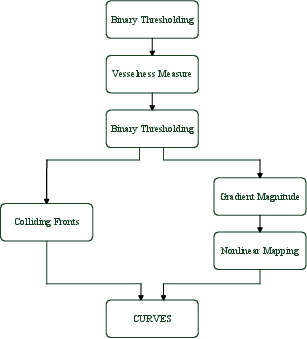
\includegraphics[height=3.2in,width=3.2in]{Figures/chap04/DataFlow.png}
\caption{Collaboration diagram of the segmentation pipeline.}
\label{fig:DataFlow}
\end{figure}

\subsection{Tubular Objects Enhancement}

The tubular enhancement is a sort of multi-scale line filtering, whose scheme can be summarized as the ``tube-like" objects in the image are highlighted whilst the rest are attenuated. %
To achieve this, the three dimensional multi-scale algorithm proposed by Sato \textit{et al.} \cite{Sato1998} is introduced.

To shape the filter response to certain width of lines and suppress the noisy effects, the pixels need to convolving with the second order derivatives of a Gaussian kernel.
This computation is an equivalent to the calculation of the Hessian matrix $\mathcal{H}$ of the three-dimensional image $I(\cdot)$:
\begin{gather}
\label{eqn:Hessian}
\mathcal{H} = \nabla^2 I =
\begin{bmatrix}
I_{xx} & I_{xy} & I_{xz} \\ I_{yx} & I_{yy} & I_{yz} \\ I_{zx} & I_{zy} & I_{zz}
\end{bmatrix},
\end{gather}
where $I_{xx} = \frac{\partial^2 I}{\partial^2 x}$, $I_{xy} = \frac{\partial^2 I}{\partial x \partial y}$, to name a few.
And all these partial second order derivatives are the convolutions with the second order derivatives of a Gaussian kernel $G(x; \sigma)$ with the standard deviation $\sigma$:
\begin{equation}
\label{GaussianConvolution}
I_{xx} = I \ast \frac{\partial^2 G}{\partial^2 x}.
\end{equation}
The eigenvalues of (\ref{eqn:Hessian}) are $\lambda_1$, $\lambda_2$, and $\lambda_3$ with their values in descending order.
Their associated eigenvectors are $e_1$, $e_2$, and $e_3$, respectively.

When $\lambda_1 \approx 0$ and $\lambda_2 \approx \lambda_3 \ll 0$, the line measure can be written as
\begin{equation}
\label{eqn:LineMeasure}
\lambda_{123} =
\begin{cases}
\left| \lambda_3 \right| \left( \frac{\lambda_2}{\lambda_3} \right)^{\gamma_{23}} \left( 1 + \frac{\lambda_1}{\left| \lambda_2 \right|} \right)^{\gamma_{12}}, & \lambda_1 \le 0 \\
\left| \lambda_3 \right| \left( \frac{\lambda_2}{\lambda_3} \right)^{\gamma_{23}} \left( 1 - \alpha \frac{\lambda_1}{\left| \lambda_2 \right|} \right)^{\gamma_{12}}, & \frac{\left| \lambda_2 \right|}{\alpha} > \lambda_1 > 0 \\
0, & \text{otherwise}.
\end{cases}
\end{equation}
In (\ref{eqn:LineMeasure}), the additional parameters $\gamma_{12}$, $\gamma_{23}$, and $\alpha$ are all positive constant, where $\gamma_{12} \in [0, \infty)$ is used to discriminate between the branching structures and the noises as well as pseudo-branches, $\gamma_{23} \in [0, \infty)$ regulates the sharpness, and $\alpha \in (0, 1.0]$ maintains the asymmetrical characteristics of the last terms of the function for all possible $\lambda_1$.

Additionally, different choices of the eigenvalues can equip the line filter with the abilities in detecting different shapes of the objects as shown in Table. \ref{tbl:Eigenvalues}. %

\subsection{Preprocessing for Level Set Evolution}

\subsubsection{Speed Images Calculation}

Level set algorithms evolves the contours in the gradient field with ``sharp" variations in intensity values from the inner or outer area to the boundaries.
The aim of the speed images is to provide this gradient field in the form of nicely shaped gradient images.
In the gradient images, the magnitude of the gradient at each pixel is calculated.
Next the gradient images $I_{\nabla}$ are transformed into the speed images $I_{\sigma}$ by applying the nonlinear relation:
\begin{equation}
\label{eqn:Sigmoid}
I_{\sigma} = (I_{max} - I_{min}) \cdot \frac{1}{1 + \exp\left(-\frac{I_{\nabla} - n}{m}\right)} + I_{min},
\end{equation}
where $I_{max}$ and $I_{min}$ are the two extreme values of the output intensity values, $m$ is a constant that controls the window width of the input intensity, and $n$ is a constant that defines the center of the window.
\begin{table}
\renewcommand{\arraystretch}{1.3}
\caption{Eigenvalue sets for detecting different shapes}
\label{tbl:Eigenvalues}
\centering
\begin{tabular}{l||c}
\hline
\bfseries Shape & \bfseries Eigenvalues \\
\hline\hline
Bright tubes   & $\lambda_1 \approx 0, \lambda_2 \approx \lambda_3 \ll 0$ \\
Dark tubes     & $\lambda_1 \approx 0, \lambda_2 \approx \lambda_3 \gg 0$ \\
Bright plates  & $\lambda_1 \approx \lambda_2 \approx 0, \lambda_3 \ll 0$ \\
Dark plates    & $\lambda_1 \approx \lambda_2 \approx 0, \lambda_3 \gg 0$ \\
Bright spheres & $\lambda_1 \approx \lambda_2 \approx \lambda_3 \ll 0$ \\
Dark spheres   & $\lambda_1 \approx \lambda_2 \approx \lambda_3 \gg 0$ \\
\hline
\end{tabular}
\end{table}

\subsubsection{Initial Contours Evolution Using Colliding Fronts}

The aim of the colliding fronts module is to evolve the contours for the CURVES system from the user-defined seeding points.
The colliding fronts method is implemented based on the principles of the fast marching algorithm \cite{Sethian1999}.
However, this method requires two seeds for each round of evolution such that the area between the seeds can be extracted.
The output of this module is the dot production of the gradient field of arrival times of the two wavefronts.
The level set initialization for the prolonged objects greatly benefit from this feature of the method.
On the other hand, the method also shortens the computation time.

\subsection{CURVES Evolution Model}

The CURVES method \cite{Lorigo2001} is chosen as the functioning segmentation method because of the complex nature of the coronary arteries.
It is highly effective in the segmentation of the complicated curvilinear structures in the volumetric medical images.
In addition, the criterion of CURVES method also takes the local smoothness of the boundaries to be detected (i.e., the inner wall of the coronary arteries) into account.

This method is a modification of the geodesic active contours method developed in Caselles \textit{et al.} \cite{Caselles1997}.
As the extensive research of the geodesic active contours, CURVES is a level set algorithm that models the tiny vessels as spatial curves with arbitrarily complicated topology \cite{Lorigo2001}. %
CURVES evolves the level sets to the boundaries of the targets based on the criterion of the minimization of the following energy functional
\begin{equation}
\label{eqn:CURVES}
\oint_0^1 g\left( \left| \nabla I \left( \mathcal{C} \left(  s \right) \right) \right| \right) \left| \mathcal{C}'\left( s \right) \right| ds,
\end{equation}
where $\mathcal{C}\left( s \right): [0,1] \rightarrow \mathrm{R}^3$ is a one-dimension curve, $I\left( \cdot \right): [0, a] \times [0, b] \times [0, c] \rightarrow [0, \infty)$ is an image on which the curve evolution takes place, and $g\left( \cdot \right): [0, \infty) \rightarrow \mathrm{R}^+$ is a monotonically decreasing function. %

The minimization of this functional can be achieved by searching for the gradient descent direction of the functional itself, which means the Euler-Lagrange equations associated with (\ref{eqn:CURVES}) needs to be computed. %
Thus the geodesic flow equation that controls the contour evolution in this process of minimization can be obtained as follows
\begin{equation}
\label{eqn:Evolution}
\frac{\partial \mathcal{C}}{\partial t} = k \mathcal{N} - \frac{g'}{g} \varPi \left( \mathcal{H} \frac{\nabla I}{ \left| \nabla I \right| } \right),
\end{equation}
where $\mathcal{H}$ is the Hessian matrix of the image $I$, $k$ is the Euclidean curvature, $\mathcal{N}$ is the unit normal vector, $\varPi(\cdot)$ is the projection operator projects the argument onto the normal space. %
The update equation can be obtained as
\begin{equation}
\label{eqn:Update}
\frac{\partial v}{\partial t} = \mathcal{F} \left( \nabla v(x, t), \nabla^2 v(x, t) \right) + \frac{g'}{g} \nabla v(x, t) \mathcal{H} \frac{\nabla I}{ \left| \nabla I \right| },
\end{equation}
where $v(\cdot): \mathrm{R}^3 \rightarrow [0, \infty)$ is the embedding function of the curve $\mathcal{C}$, $\mathcal{F} \left( \nabla v(x, t), \nabla^2 v(x, t) \right)$ is the smaller eigenvalue of the matrix $P_{\nabla v} \nabla^2 v P_{\nabla v}$. %
The matrix $P_q$ is defined as a projector which projects some vector onto the normal plane of vector $q \in \mathrm{R}^3$:
\begin{equation}
\label{eqn:ProjectionOperator}
P_q = I_0 - \frac{qq^T}{\left| q \right|^2},
\end{equation}
where $I_0$ denotes the identity matrix.

By incorporating the speed images $I_{\sigma}$ to the evolution equation (\ref{eqn:Evolution}), the evolution in our case can be obtained as
\begin{equation}
\label{eqn:Application}
\frac{\partial \mathcal{C}}{\partial t} = k \mathcal{N} - \frac{g'(I_{\sigma})}{g(I_{\sigma})} \varPi \left( \mathcal{H} \frac{\nabla I_{\sigma}}{ \left| \nabla I_{\sigma} \right| } \right).%
\end{equation}

\subsection{Surface Rendering}

The surface information is extracted for the visualization by the marching cubes method \cite{Lorensen1987MC}.
Cubes are created based on the input information and are organized into an array structure.
Each cube consists of eight pixels (each four pixels are from a slice).
The index of each cube is labeled by comparing the intensity values of every pixel to the isovalue of the surfaces.
Next the patterns of the intersection between objects and cubes are initially determined based on the triangulated cases.
Then the precise intersection are computed using linear interpolation with the intensity values at each vertex.
The unit normals to the surface are calculated via central differences for the vertices of the cubes.
Finally the generated triangles are ready for the surface rendering.

\section{Experiments and Results}

\subsection{Medical Data and Experimental Setup}

The original chest CTA series was acquired by a 128-slice Siemens SOMATOM Definition Flash CT.
The slice thickness was $0.6 \text{mm}$ and the in-slice resolution was $0.4 \times 0.4 \text{mm}^2$.
Since the work was all on the coronary arteries, the volume contained the whole heart (i.e., ROI, which is the abbreviation of \textit{region of interest}) was cropped from the original data as shown in Fig. \ref{fig:Original}. %

Numbers of experiments were conducted with different sets of parameters to segment the coronary arteries from CTA for the testament of the approach in this paper.
In our case, the original CTA series in DICOM format had been converted to the form of XML first; and the data type of pixels are converted for the incoming computation.
Next the converted data was enhanced by the module which was implemented based on the algorithm developed in \cite{Sato1998}.
Then the tubular enhanced data was send to the following modules to perform calculations of speed image production and input level sets generation.
The two set of the resulting data from the two computation pipelines were transferred to the CURVES module in order to generate the final fronts evolution results.
Finally, the marching cubes method was employed to extract the iso-surface corresponding to the wall of the coronary arteries.
All the experiments were performed on a machine with Intel's 2.83GHz Core 2 Quad CPU and 4GB RAM.

\subsection{Tubular Enhancement and Its Postprocessing}

Before the tubular enhancement started, a global binary thresholding was performed in order to provide the enhancing filter with the focus on the tiny bright tubular objects.
To achieve this, the thresholder was called to trim the irrelevant contents in the images, e.g., dark lung regions with negative intensity values, bright bone regions with large positive intensity values, etc. %
As shown in Fig. \ref{fig:Binary1}, the intensity values of the regions within the interval between the lower threshold and the upper threshold were uniformly assigned a unique intensity value, i.e., $255$ in our case; the intensity values of the rest regions were uniformly assign a zero intensity value. %

Referring to the shape prior guidelines listed in Table. \ref{tbl:Eigenvalues}, the tubular enhancement filter was fed the parameters to detect the bright tubular objects, i.e., coronary arteries. %
Among these parameters, $\sigma$ controls the diameter of cross-section of the tubular objects to be enhanced, $\gamma_{12}$ is the measure of the tube similarity, and $\gamma_{23}$ is used for the recovery of vessel regions with inhomogeneous contrast or intensity loss. %
As shown in Fig. \ref{fig:Vesselness}, the tiny vessels including the coronary arteries and the vessels in lung areas were enhanced with a small $\sigma$ whilst the tubular structures with cross-section diameters larger than this value were not enhanced. %

The intensity values of the enhanced tubular objects were relatively low and scattered in a wide range.
This is a mass for the selection of the intensity value in the following processing steps.
To deal with it and facilitate this situation, some intensity transformation step was needed.
The nonlinear intensity mapping filter and the binary threshold filter were the candidates.

Equation (\ref{eqn:Sigmoid}) showed that the nonlinear intensity mapping transformed the input image into the image with partial enhancement and partial attenuation.
With the well chosen parameters, the intensity values corresponding to the targeting objects in this case were enlarged and the rest part of the images in lower intensities were all depressed as near zero intensity areas. %
Because of the mapping characteristics of the sigmoid functions, the intensity values of the bright tubular structures were not uniformly distributed and stayed at the relatively low levels (see Fig. \ref{fig:Sigmoid}). %
In another test, the binary threshold filter extracted the pixels with the intensities in the specified range and assigned them with a unique large intensity value as discussed above (see Fig. \ref{fig:Binary2}). %
Comparing the result of the two candidates, the binary threshold filter was selected to improve the results of the precedent tubular enhancement filter (see Fig. \ref{fig:DataFlow}). %
\begin{figure}[t]
\centering
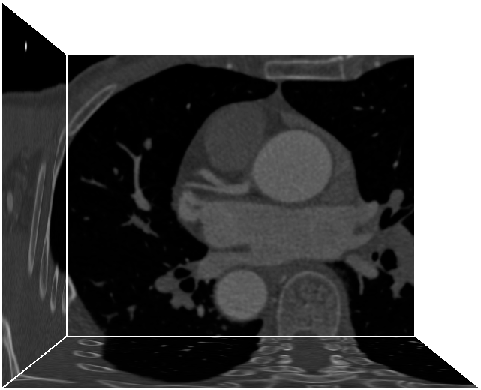
\includegraphics[width=2.8in]{Figures/chap04/original.png}
\caption{Original ROI-extracted volumetric data}
\label{fig:Original}
\end{figure}
\begin{figure}[t]
\centering
\subfloat[]{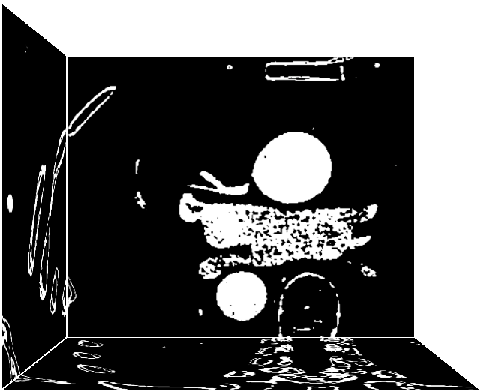
\includegraphics[width=2.8in]{Figures/chap04/binary1.png}%
\label{fig:Binary1}}
\hfil
\subfloat[]{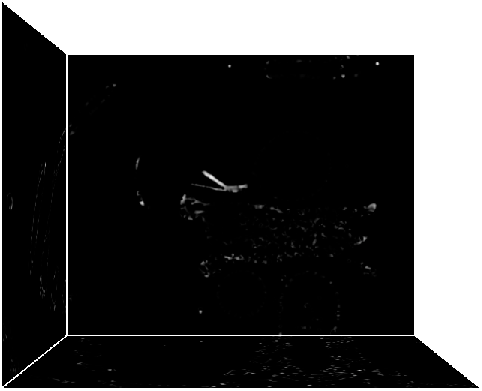
\includegraphics[width=2.8in]{Figures/chap04/hessian.png}%
\label{fig:Vesselness}}
\caption{Preprocessing results of the original CTA images based on the ``vesselness" measure: (a) binary thresholding ($\text{lower threshold} = 300$, $\text{upper threshold} = 600$) (b) tubular enhancement ($\sigma = 0.9$, $\gamma_{12} = 0.1$, $\gamma_{23} = 2.0$).}%
\label{fig:Preprocessing}
\end{figure}

\subsection{Feature Images Computation}

To generate the feature images for the CURVES system, two steps were performed:
(1) calculating the gradient magnitude at each pixel; and
(2) converting the gradient images into the speed images.
%\begin{enumerate}
%\item calculating the gradient magnitude at each pixel;
%\item converting the gradient images into the speed images.
%\end{enumerate}
The gradient magnitude module computed the magnitude of the gradient pixel-wisely for the image by performing the convolution with the first order derivatives of a Gaussian kernel.
The wall of the tiny vessels were extracted before the nonlinear intensity mapping was employed to generate the edge potential maps.
The extreme values of the pixel intensities in the gradient magnitude images directly effected the selection of the parameters in (\ref{eqn:Sigmoid}).
To reverse the lightness of the objects (in low intensities in the gradient magnitude images) and its edges (in high intensities in the gradient magnitude images), $n$ was chosen to be the center of the intensity window containing the vessels, and $m$ a negative value with $|m|$ as the width of the window. %
The minus sign of $m$ means the reverse operation on the pixels.
The neighborhood of the boundaries of the objects were in almost zero intensity, which made the evolution driven by (\ref{eqn:Application}) faster in the ``plateau" (with uniformly high intensities), whilst much slower (in a speed of about zero) in the ``ridges" (with rapid decreasing intensities). %

\subsection{Wave Fronts Propagation}

The initial level sets were evolved by the colliding fronts module.
Two seeds were located interior of the regions corresponding to the coronary arteries and the interfaces surrounding each seeds evolved towards each other.
The dot production of the gradients of arrival times of the two wavefronts were computed.
\begin{figure}[t]
\centering
\subfloat[]{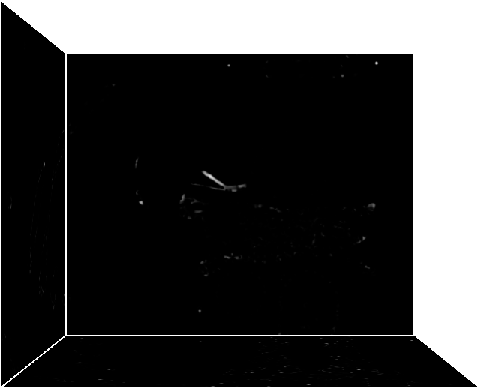
\includegraphics[width=2.8in]{Figures/chap04/sigmoid.png}%
\label{fig:Sigmoid}}
\hfil
\subfloat[]{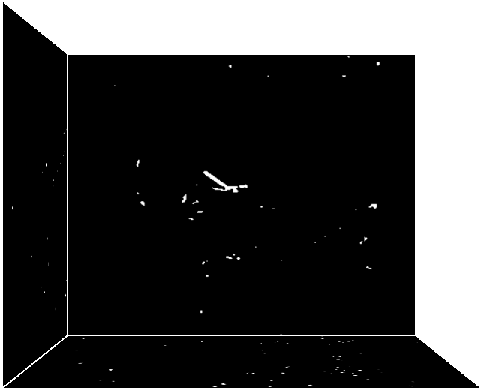
\includegraphics[width=2.8in]{Figures/chap04/binary2.png}%
\label{fig:Binary2}}
\caption{Comparison of the two different intensity conditioning approaches: (a) nonlinear intensity mapping ($m = 80$, $n = 120$); (b) binary thresholding ($\text{lower threshold} = 40$, $\text{upper threshold} = 200$).}%
\label{fig:IntensityConditioning}
\end{figure}
\begin{figure}[t]
\centering
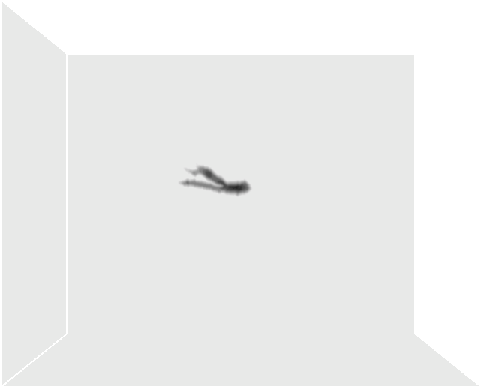
\includegraphics[width=2.8in]{Figures/chap04/curves.png}
\caption{CURVES evolution based on the initial contours generated by the colliding fronts method and the edge feature maps calculated by the nonlinear intensity mapping function.}%
\label{fig:CURVES}
\end{figure}
\begin{figure*}[t]
\centering
\subfloat[]{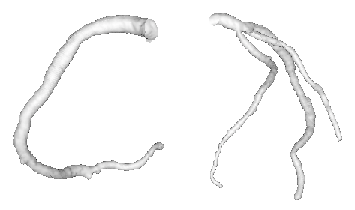
\includegraphics[width=2.8in]{Figures/chap04/model_conventional.png}%
\label{fig:VisualizationModelCURVES}}
\hfil
\subfloat[]{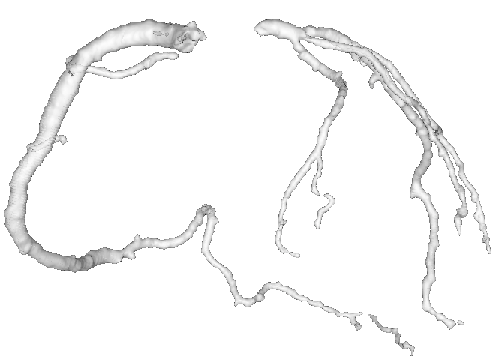
\includegraphics[width=2.4in]{Figures/chap04/model_enhanced.png}%
\label{fig:VisualizationModelTECURVES}}
\caption{Models of the coronary arteries: (a) conventional CURVES evolution; (b) tubular-enhanced CURVES evolution.}%
\label{fig:VisualizationModel}
\end{figure*}

The CURVES system started working when all the preceding calculation completed.
The module took the speed images as its evolution maps and the initial contours as its initial states and regulates the evolution according to (\ref{eqn:Application}).
The evolution terminated when the contours evolved against the wall of the coronary arteries in the specified steps of iterations.
And the resulting evolution extracted the coronary arteries as shown in Fig. \ref{fig:CURVES}.
Next a binary thresholding step was provoked to label the inner area of the coronary arteries with high intensity value whilst the outer area with zero intensity value.

\subsection{Visualization of Segmentation Results}

By manually picked the isovalue corresponding to the wall of the coronary arteries, the resulting volume were processed using the marching cubes method \cite{Lorensen1987MC}.
The visualization models of the coronary arteries respectively based on the CURVES regions without and with tubular enhancement demonstrated their capabilities of displaying the complicated geometrical details (see Fig. \ref{fig:VisualizationModelCURVES} and \ref{fig:VisualizationModelTECURVES}). %

\section{Conclusions and Future Work}
%The conclusion goes here.

The three dimensional visualization of the blood vessels plays an important role in the construction of the virtual scenario for the robotic surgical simulator.
Further, the visualization of the coronary arteries is the most critical and difficult work.
Because of the complex spatial topologies, details can be easily lost in the process of segmentation.
In this paper, a vasculature segmentation method based on tubular-enhanced CURVES has been developed.
Then the process of the experiment was presented and the results were demonstrated.
The experimental results showed that the proposed approach is capable of enhancing the tiny dark vessels and visualizing the geometric details of them.

The tubular feature of coronary arteries was enhanced and the speed images were generated.
Meanwhile, the initial contours for the CURVES method were computed by a modified version of fast marching method in another process.
The actual level sets evolution began after the above computation finished and the evolution took a specified number of iterations to detect the coronary arteries.
At the end of the segmentation, the resulting pixels were all conversed in their intensities.
Finally the data representing the surface of the arteries was extracted by the marching cubes method.

Our future plans are the further optimization of the blood vessel models for the simulation with virtual tools of the robotic surgical simulator.
The principle work will be the decimation of the quantity of the triangles consisting the blood vessels and the improvements of the visualization effects of the virtual scenario. 
%# -*- coding:utf-8 -*-
\chapter{血管模型中心线的提取}
\label{chap7}

\section{Introduction}
% no \PARstart
Cardiovascular diseases are among the most fatal illnesses worldwide \cite{WHO2013}.
The diseases occur when the stenosis or even blockages formed due to the build up of fatty substances on the inner wall of the blood vessels.
Percutaneous coronary intervention (PCI) is the gold standard in fighting the lethal diseases.
Due to its minimally-invasive nature, this procedure only causes small incision and much less trauma to the patients.
In addition, the hospitalization after the procedure is in turn dramatically shortened.
However, due to the very nature of minimally-invasiveness of PCI and the complex anatomic structure of the blood vessels, the learners need thorough and strict training before performing the procedure in action. %
What's worse, the practitioners in catheterization labs have to expose themselves under the ionizing radiation from the fluoroscope while examining the morphologies of the patients' vasculature. %

The surgical robotic systems for intravascular procedures have greatly changed this situation.
With the assistance of the robotic systems, cardiology practitioners need not to be worried about the radioactive exposure and the relative risks any more.
Like their ancestors (i.e., the traditional PCI procedure), the skills of manipulating the robotic system to do the surgery are also not easy for the junior residences and still require strict and sufficient training before applying the procedure on the real patients. %

The traditional ways of training PCI procedure are deeply rooted in the physical fashion, i.e., employing biological models (e.g. human cadavers and living animals) or non-biological models (e.g. phantoms). %
The former are disposable and ethic-disputed; let alone the tremendous expenditure on the preservation and feeding, and the distinction in anatomy between human and animal volunteer. %
The latter are stiff and lack of sufficient anatomic details, even though they can be used repeatedly.
Indeed, it is infeasible to conduct the training on the expensive robotic systems whilst ignoring the real needs in the catheterization labs.
To streamline the training and the practice of robotic PCI procedure, a well-designed computing simulation system is required.

The aim of our effort is to provide a training tool of convenience and effectiveness for the minimally-invasive intravascular robotic system \cite{Ji2011EMBC}.
In constructing this training vehicle, the anatomic structures in computing environment especially the vascular system are definitely one of the most substantial components.
The centerlines is an effective way of describing the shape of the model \cite{Ogniewicz1995}, which will provide accurate shape description for the path planning in interactive simulation.
In this paper, we developed an automatic approach based on the Voronoi diagram \cite{Antiga2003} to extract the centerlines of the vasculature.
The input of the proposed approach is the patient-specific image-based surface model of the vasculature, which is reconstructed by applying our previous work \cite{Yang2014ICRA}. %
Before computing the Voronoi diagram of the tubular surface model, several preprocessing should be performed.
First, the connectivity of the polygons that consisting the surface is validated thoroughly to include the largest connected polygons that is effective in representing the surface. %
Second, the bumpy and crusty surfaces are smoothed in order to reduce the effects on the computation of centerlines.
Third, the surfaces are subdivided to gain a more precise geometric feature.
Finally, the centerlines of the vessel model by solving the Eikonal equation in the fast marching flavor.
The capability of our approach in automatically extracting the centerlines of the vessel model is proved by the experimental results.

The rest of this paper is organized as follows.
Section II introduces the related work of the centerline extraction methods for three dimensional objects.
Section III outlines the work flow and describes the techniques used in this work.
Section IV describes the experiments, ending with a brief discussion.
The final section concludes the whole work.

\section{Related Work}

Many researches have been done since the earliest work on extracting the centerline was proposed by Blum \cite{Blum1967}.
According to reference \cite{Ogniewicz1995}, most of these methods fall into four categories: (1) topological thinning; (2) distance transformation; (3) ``prairie fire" approach; (4) Voronoi Diagram methods. %

Topological thinning methods \cite{Ma2002,Sadleir2002} implement the centerline extraction by iteratively remove most of the ``simple points" except the ones that are the end-points of the generated centerline models. %
By ``simple points", it means that the boundary points consisting the object such that their removals do not destroy the topology of the object.

Distance transformation methods \cite{Niblack1992} find the centerline by searching the local maximum among the minimal distances between the points interior of the shape and the boundary. %
However, they do not ensure the resulting centerlines are connected with each other.

``Prairie fire" methods \cite{Blum1967,Leymarie1992} compute the centerline by determining the intersection of the propagating interfaces with their sources located on the boundary of the shape. %

Voronoi diagram method \cite{Sherbrooke1996,Antiga2003} treats the centerline to be generated as a subset of the Voronoi diagram.
These methods are sensitive to the noises and the regularization of the boundary of the shape.

There are numbers of other methods that are not belong to any category listed above.
Ferchichi and Wang in \cite{Ferchichi2006} reported a clustering-based algorithm for centerline extraction both for 2D and 3D objects.
The algorithm was designed based on the idea of computing the maximal disks/balls determining the centerlines, which is achieved by executing the K-means algorithm iteratively on the object-points and their distance transforms. %
Egger \textit{et al.} \cite{Egger2007} reported a centerline extraction algorithm for the blood vessels using Dijkstra's shortest path algorithm, which was designed for the catheter simulation. %

\section{Methodologies}

This section discusses the design of the processing pipeline and details the principles of the consisting modules.
Before the actual centerline extraction begins, several processing aims to removing noises and smoothing the irregular surfaces need to be run to guarantee the quality of the input surface.
The image-based surface model of the blood vessels needs series of postprocessing steps depicted in Fig. \ref{fig:DataFlow} to meet the requirements of the centerline computing module. %
Among these processing steps, the first one is the validation of the connectivity of the consisting polygons.
During this process, the largest possible connected regions of the surface model are extracted.
Next, the surface smoothing step is needed to depress the ``crusts" and ``stairs" in the surface.
Then the normal vectors (i.e., normals) are computed to mark the ``inside" and the ``outside" of the surface model.
After that, the consisting polygons need to be subdivided under a specified criterion to facilitate the computation of the centerline extraction at the cost of longer computation time. %

%\subsection{Processing on Image-Based Surface Model}

\subsection{Connectivity Validation and Largest Region Extraction}

In this paper, the vasculature surface model is generated from the original medical volumetric data set by applying the approaches reported in our previous work \cite{Yang2014ICRA}. %
In order to find the largest region spanning the surface of the vasculature, the connectivity among the vertices in the image-based surface model needs to be thoroughly validated at the beginning of the processing. %
The inner working is to extract consisting polygons that share common vertices and meet some requirements.
In the present paper we implement the algorithm to extract the largest connected region from the input surface.
\begin{figure}[t]
\centering
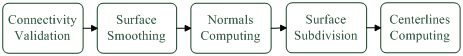
\includegraphics[width=3.2in]{Figures/DataFlow3.png}
\caption{Overview of the work flow.}
\label{fig:DataFlow}
\end{figure}

\subsection{Surface Smoothing and Normals Computing}

There are plenty of methods used for the surfaces smoothing in visualization.
To overcome the ``facets" by-produced during this approximation, an optimal surface smoothing algorithm treating this problem as low-pass filtering by extending Fourier analysis is adopted \cite{Taubin1996}. %
The adopted method is built upon the formulation of the \emph{discrete graph signals}, which means the functions based on directed graph.
The directed graph $G$ represents the polyhedral surfaces in this problem, which is denoted as the set $\left\{ 1, \ldots, n \right\}$ of nodes with a set of neighborhoods $\left\{ i^{\ast}: i = 1, \ldots, n \right\}$ of node $i$. %
A discrete graph signal can be represented as a vector $x = \left[ x_1, \ldots, x_n \right]^T$, where each component of the vector corresponds one node of the graph.
A polyhedral surface $S = \{ V, F \}$ of $n$ vertices can be treated as a directed graph, where the vertices $V$ corresponds the set of nodes $n$ and the faces $F$ the polygons formed by connected nodes. %

The discrete surface signal, the discrete graph signal defined on the associated graph, can be visualized as a piece-wise linear function defined on the surface.
The computation of the Discrete Fourier Transform (DFT) of the discrete surface signal defined on the surface is achieved by decomposing the surface signals as a linear combination of the eigenvectors of the Laplacian: %
\begin{equation}
\label{eqn:Laplacian}
\Delta x_i = \sum_{j \in i^{\ast}} w_{ij} \left( x_j - x_i \right),
\end{equation}
where $w_{ij}$ is the positive weight for each difference of $x_j - x_i$ and for a given vertex $i$, the sum of its weights are always one.
The matrix form of (\ref{eqn:Laplacian}) is
\begin{equation}
\label{eqn:LaplacianMatrix}
\Delta x = - K x,
\end{equation}
where $K = I - W$, with $I$ an identity matrix and $W$ the matrix of weights $w_{ij}$.

Choosing $0 \leq k_1 \leq \ldots \leq k_n \leq 2 $ as the eigenvalues of $K$, $r_1, \ldots, r_n$ the corresponding right eigenvectors, and $d_1, \ldots, d_n$ the associated dual basis of these eigenvectors, the above $K$ can be obtained as $K = \sum_{i} k_i r_i d_i^T$. %
%\begin{equation}
%\label{eqn:K}
%K = \sum_{i} k_i r_i d_i^T.
%\end{equation}
Thus there is a unique decomposition the discrete graph signal $x$, which can be obtained as a linear combination of the right eigenvectors $x = \sum_{i} \hat{x}_i r_i$, %$r_1, \ldots, r_n$
%\begin{equation}
%\label{eqn:x}
%x = \sum_{i} \hat{x}_i r_i,
%\end{equation}
where $\hat{x}_i = d_i^T x$ is the DFT of $x$.

According to signal processing theory, the filtering calculation on the signal $x$ is to change its frequency distribution at the reference of a transfer function $f$:
\begin{equation}
\bar{x} = \sum_{i} f(k_i) \hat{x}_i r_i = \left( \sum_{i} f(k_i) r_i d_i^T \right) x.
\end{equation}
The \emph{low-pass filtering} mechanism can be implemented by adjusting the weights in the following polynomial approximation
\begin{equation}
\label{eqn:Approximation}
f_{N}(k) = w_0 \frac{\theta}{\pi} T_0 (1 - k / 2) + w_n \sum_{n} \frac{2 \sin (n \theta)}{n \pi} T_n(1 - k / 2),
\end{equation}
where $\theta$ is the unique solution of $k = 2 (1 - \cos \theta)$ on $[0, \pi / 2]$, and $T$ the Chebyshev polynomial.
Here in this paper, the weights in (\ref{eqn:Approximation}) is adjusted to form a Hamming window, among sorts of them, which is demonstrated as follows:
\begin{equation}
\label{eqn:HammingWindow}
w_n = 0.54 + 0.46 \cos (n \pi / (N + 1) ).
\end{equation}

The normal vectors to the surfaces are computed after the surfaces are smoothed.

\subsection{Surface Subdivision}

A modified butterfly scheme for surface subdivision is used in order to refine the smoothed surface model \cite{Zorin1996}.
This scheme is designed in the flavor of interpolating and has been proved to be useful in the circumstances of subdivision for the complex especially irregular surfaces.
The ultimate goal is to improve the visualization of the input surface model without affecting its original shape.
The scalar value associated with the new vertex of the 2-dimensional triangulation is generated by calculating weighted sum of neighboring vertices using the proposed interpolation scheme. %
These vertices located in the neighborhood form the subdivision stencil, which determines the features of the scheme.
By analyzing the stencil, the scheme can quickly identify the relationship between the new vertex and the topology of its neighborhood.
The two most important cases in the surface are the regular sites and the extraordinary sites.
Once the initial subdivision cycles completed, the largest number of the vertices possessing the valence other than six is not exceeding one.
The new scalar value for the midpoint on each edge of the triangulation is calculated by the subdivision scheme falls into the following cases:
(1) edge connects two regular vertices;
(2) edge connects an extraordinary vertex and a regular vertex;
(3) edge connects two extraordinary vertices; and
(4) boundary edges.
%\begin{itemize}
%\item edge connects two regular vertices;
%\item edge connects an extraordinary vertex and a regular vertex;
%\item edge connects two extraordinary vertices;
%\item boundary edges.
%\end{itemize}
Among the above cases, only the first one belongs to the regular case, whilst the rest belong to the extraordinary case.

\subsection{Centerlines Extraction}

Centerlines, or medial axis, can be generally defined as the loci of the centers of the maximal inscribed disks (in 2D space) or spheres (in 3D space) inside an object.
Conversely, the envelop of all maximal inscribed disks/spheres is the boundary/surface of the object that contains these disks/spheres \cite{Amenta2001}.
Our approach employed the method demonstrated in \cite{Antiga2003}, which treats the centerlines as the minimal action paths on the Voronoi diagrams inside the model surface.
The Voronoi diagrams are the discrete approximation of the medial axis of the shape in two or three dimensional space.
The minimization of the line integral of the action path, which links two vertices in the Voronoi diagram, generates the center points that locally maximize their minimal distances to the boundary of the surface.
To do this, the method firstly computes the following Eikonal equation from a given starting point located on the Voronoi diagram
\begin{equation}
\label{eqn:Voronoi}
\left| \nabla T \right| = \frac{1}{R(u)},
\end{equation}
where $T$ marks the time of arrival, $R$ the radius of the maximal inscribed sphere at the time $T$, and $u$ the parametric space of the Voronoi diagram.
Then the centerline is obtained by calculating the following equation upon the previously demonstrated computation terminated:
\begin{equation}
\label{eqn:Centerlines}
\frac{dc}{ds} = - \nabla T,
\end{equation}
where $c$ denotes the centerlines, and $s$ the parametric space of $c$.
As a matter of fact, computation illustrated by (\ref{eqn:Centerlines}) is equivalent to finding the resulting centerline by applying the steepest descent method at each point on the Voronoi diagram.

\section{Experiments and Discussions}

\subsection{Data and Experimental Setup}

The vasculature surface models were generated by applying the approaches proposed in \cite{Yang2014ICRA} from the original CTA images acquired from some real patient.

In our experiments, the programs written in C++ ran on a desktop with Intel's 2.83GHz Core 2 Quad CPU and 4GB RAM.
%For the simplicity of description, part of the abdominal aorta is chopped off to serve as the sample data in our experiments described here (see Fig. \ref{fig:VOI}). %
Part of the abdominal aorta was chopped off to serve as the sample data in our experiments described here (see Fig. \ref{fig:VOI}). %
The approach can be applied straightly to the surface model of the whole abdominal aorta (see Fig. \ref{fig:OverlayGlobal}). %and Fig. \ref{fig:VisualizationModel}).
\begin{figure}[t]
\centering
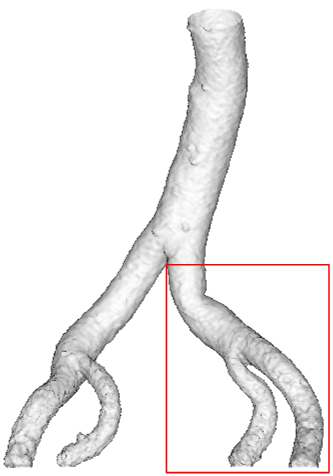
\includegraphics[height=2.4in]{Figures/VOI.png}
\caption{The original model surface (consists of $205,590$ polygons) and the VOI-extracted local part (in red square).}
\label{fig:VOI}
\end{figure}

%\subsection{Preprocessing for Centerline Extraction}

\subsection{Validating Connectivity of Image-Based Surface Model}

Before actually extracting the centerlines, the image-based surface model of the vasculature needs to be properly conditioned such that the computation can be operated successfully. %
The initial pass is the validation of the connectivity among the adjacent polygonal surfaces that consists of the whole visualization model.
The aim of this step is to find and connect the largest connected region in the given surface model (see Fig. \ref{fig:ConnectivityLocal}).
Table \ref{tbl:Connectivity} shows that the quantities of the consisting polygonal surfaces were not changed in local cases, whilst were decreased in global cases.
The former implies that the given (local) model was the largest connected region in the surface model before the validation.
The latter indicates that the largest connected region of the given model surface was fully extracted through the validation.
\begin{figure}[t]
\centering
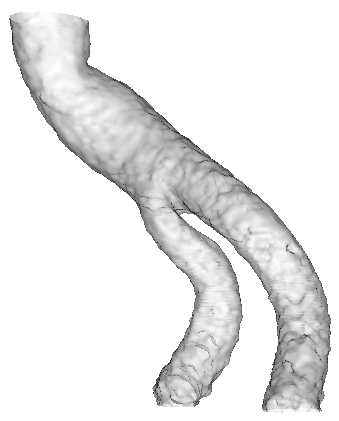
\includegraphics[width=1.5in]{Figures/connectivity_local.png}
\caption{Results of connectivity validation of model surface in local details (quantity of consisting polygons: $70,625$).}
\label{fig:ConnectivityLocal}
\end{figure}

\begin{table}[t]
\renewcommand{\arraystretch}{1.3}
\caption{Quantities of polygons before and after connectivity validation}
\label{tbl:Connectivity}
\centering
\begin{tabular}
{@{}llr@{}}
%{@{}llrr@{}}
\toprule
%\hline
%~      & ~                       & \multicolumn{2}{c}{Quantities} \\
%\cmidrule(4){3-4}
%~      & ~                       & Vertices & Polygons            \\
~      &                         & Quantities of polygons \\
%\midrule
\hline\hline
%Local  & Before validation       & N/A      & 70,625  \\
%~      & After validation        & N/A      & 70,625  \\
Local  & Before validation       & $70,625$  \\
~      & After validation        & $70,625$  \\
\hline\hline
%Global & Before validation       & N/A      & 205,590 \\
%~      & After validation        & N/A      & 205,452 \\
Global & Before validation       & $205,590$ \\
~      & After validation        & $205,452$ \\
\bottomrule
%\hline
\end{tabular}
\end{table}
\begin{figure}[t]
\centering
\subfloat{\includegraphics[width=1.5in]{Figures/smooth_30_1_local.png}%
\label{fig:Smooth30-1Local}}
\hfil
\subfloat{\includegraphics[width=1.45in]{Figures/smooth_30_01_local.png}%
\label{fig:Smooth30-01Local}}
\hfil
\subfloat{\includegraphics[width=1.5in]{Figures/smooth_100_1_local.png}%
\label{fig:Smooth100-1Local}}
\hfil
\subfloat{\includegraphics[width=1.45in]{Figures/smooth_100_01_local.png}%
\label{fig:Smooth100-01Local}}
\caption{Smoothing effects by applying different parameters: (a) $\text{pass band} = 0.1$, $\text{iterations} = 30$; (b) $\text{pass band} = 0.01$, $\text{iterations} = 30$; (c) $\text{pass band} = 0.1$, $\text{iterations} = 100$; (d) $\text{pass band} = 0.01$, $\text{iterations} = 100$.}%
\label{fig:SmoothLocal}
\end{figure}

%\begin{table}
%\renewcommand{\arraystretch}{1.3}
%\caption{Comparison of quantities of polygonal surfaces - Part I}
%\label{tbl:Eigenvalues}
%\centering
%\begin{tabular}{l||r}
%\hline
%\bfseries Connectivity validation & \bfseries Quantities \\
%\hline\hline
%Before                            & 757,538 \\
%After                             & 757,400 \\
%\hline
%\end{tabular}
%\end{table}

\subsection{Smoothing Connected Surface Model}

The centerline extracting method adopted in this work is sensitive to the noises on the input surface.
Due to the poor quality in some level of details of the original images, segmentation may introduce unnecessary uneven surfaces.
These artifacts in the surfaces can cause difficulties in the delivering of the virtual guidewires towards the hesion along the lumen of the model vessels.
To depress the noisy surface of the model, a surface smoothing module implemented based on low-pass filtering is applied.
There are two parameters associated with the smoothing module.
One of them specifies the number of iterations, which is equivalent to the degree of the polynomial approximating the windowed sinc function defined by (\ref{eqn:Approximation}).
The other determines the pass band of this low-pass filtering module.
Different sets of parameters were fed to the smoothing module in order to find the best results for the following processing (see Fig. \ref{fig:SmoothLocal}).
Observing these results, the parameters ($\text{pass band} = 0.01$, $\text{iterations} = 100$) used to generating the resulting surface in Fig. \ref{fig:Smooth100-01Local} demonstrated better effects than the rest.
%\begin{figure}[t]
%\centering
%\subfloat[]{\includegraphics[width=1.5in]{../Figures/smooth_30_1_local.eps}%
%\label{fig:Smooth30-1Local}}
%\hfil
%\subfloat[]{\includegraphics[width=1.45in]{../Figures/smooth_30_01_local.eps}%
%\label{fig:Smooth30-01Local}}
%\hfil
%\subfloat[]{\includegraphics[width=1.5in]{../Figures/smooth_100_1_local.eps}%
%\label{fig:Smooth100-1Local}}
%\hfil
%\subfloat[]{\includegraphics[width=1.45in]{../Figures/smooth_100_01_local.eps}%
%\label{fig:Smooth100-01Local}}
%\caption{Smoothing effects by applying different parameters: (a) $\text{pass band} = 0.1$, $\text{iterations} = 30$; (b) $\text{pass band} = 0.01$, $\text{iterations} = 30$; (c) $\text{pass band} = 0.1$, $\text{iterations} = 100$; (d) $\text{pass band} = 0.01$, $\text{iterations} = 100$.}%
%\label{fig:SmoothLocal}
%\end{figure}

\subsection{Subdivision Using Improved Butterfly Scheme}

To further attenuate the effects of noisy surfaces on extraction of centerlines and increase the precision of the centerlines extraction, the number of the polygons consisting the model surface has to be increased.
In order to achieve this, the smoothed surface need to be subdivided without introducing more perturbation.
Figure \ref{fig:SubdivisionLocal} illustrates that the subdivision computation based on the improved butterfly scheme.
At the same time, the quantities of the consisting polygonal surfaces increased substantially after the subdivision complete (see Table \ref{tbl:Subdivision}).
Comparing the quantities of the polygons before and after the subdivision in both cases, the quantities of the resulting polygons are about four times greater than the quantities of the input polygons due to the subdivision scheme employed in this work.
\begin{figure}[t]
\centering
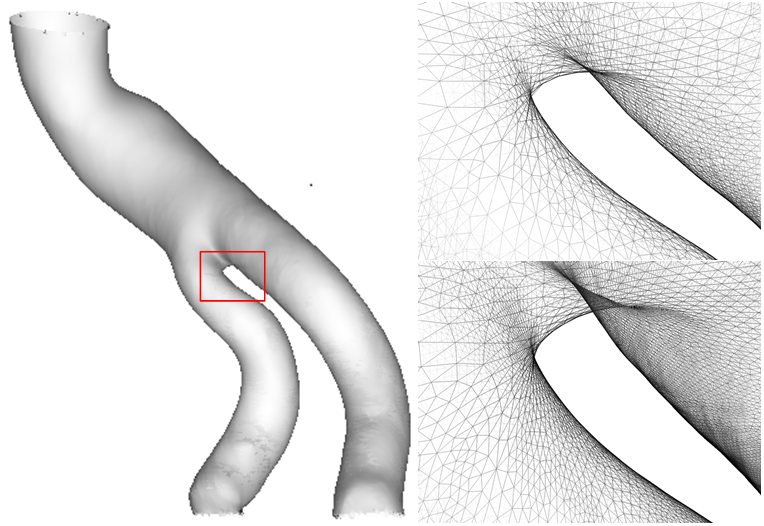
\includegraphics[width=3.0in]{Figures/subdivision.png}
\caption{Subdivision of smoothed surface by using improved butterfly scheme. \emph{Left}: subdivision in local details. \emph{Top right}: polyhedral surface before subdivision. \emph{Bottom right}: polyhedral surface after subdivision.}%
\label{fig:SubdivisionLocal}
\end{figure}

\begin{table}[t]
\renewcommand{\arraystretch}{1.3}
\caption{Quantities of polygons before and after subdivision using an improved butterfly scheme}
\label{tbl:Subdivision}
\centering
\begin{tabular}
%{@{}llr@{}}
{@{}llrr@{}}
\toprule
%\hline
%~      & ~                       & \multicolumn{2}{c}{Quantities} \\
%\cmidrule(4){3-4}
%~      & ~                       & Vertices & Polygons            \\
~      &                         & Quantities of polygons & Percentages ($\%$)\\
%\midrule
\hline\hline
%Local  & Before subdivision      & N/A      &  70,625  \\
%~      & After subdivision       & N/A      & 281,060  \\
Local  & Before subdivision      &  $70,625$  &\\
~      & After subdivision       & $281,060$  & 398 \\
\hline\hline
%Global & Before validation       & N/A      & 205,452  \\
%~      & After validation        & N/A      & 821,808  \\
Global & Before validation       & $205,452$  &\\
~      & After validation        & $821,808$  & 400 \\
\bottomrule
%\hline
\end{tabular}
\end{table}

%\begin{table}
%\renewcommand{\arraystretch}{1.3}
%\caption{Comparison of quantities of polygonal surfaces - Part II}
%\label{tbl:Eigenvalues}
%\centering
%\begin{tabular}{l||r}
%\hline
%\bfseries Subdivision  & \bfseries Quantities \\
%\hline\hline
%Before                 &  757,400 \\
%After                  & 3,029,600 \\
%\hline
%\end{tabular}
%\end{table}

\begin{figure}[t]
\centering
\subfloat{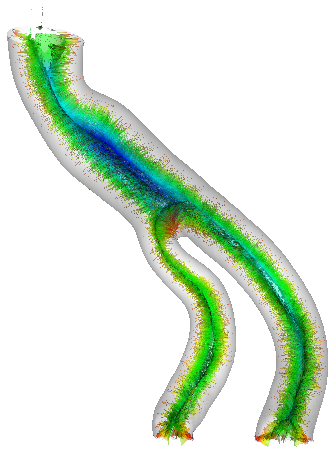
\includegraphics[width=1.5in]{Figures/overlay_100_01_voronoi_local.png}%
\label{fig:VoronoiLocal}}
\hfil
\subfloat{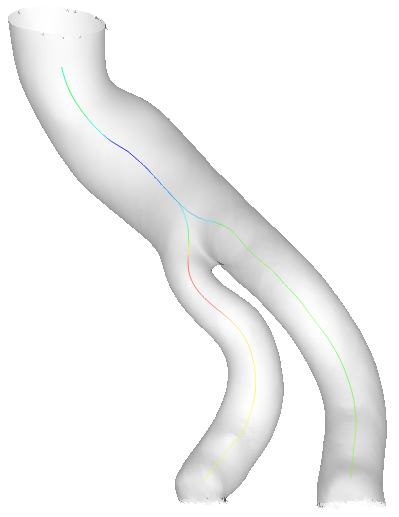
\includegraphics[width=1.5in]{Figures/overlay_100_01_centerlines_local.png}%
\label{fig:OverlayLocal}}
\caption{Centerlines extraction of the aorta in local details: (a) embedded Voronoi diagram; (b) centerlines inside the vessel.}%
\label{fig:CenterlinesLocal}
\end{figure}

\begin{figure}[t]
\centering
\subfloat{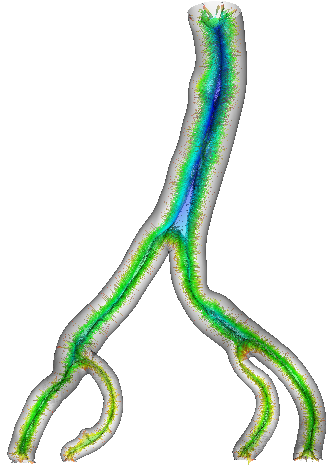
\includegraphics[height=2.0in]{Figures/overlay_100_01_voronoi.png}
%\caption{Voronoi diagrams of the abdominal aorta.}
\label{fig:VoronoiGlobal}}
\hfil
\subfloat{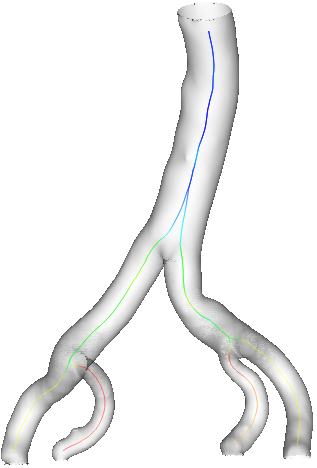
\includegraphics[height=2.0in]{Figures/overlay_100_01_centerlines.png}
%\caption{Centerlines of the abdominal aorta.}
\label{fig:OverlayGlobal}}
\caption{Centerlines extraction of the aorta in VOI. (a) Voronoi diagrams; (b) Centerlines. }
\label{fig:CenterlineGlobal}
\end{figure}

\subsection{Centerlines Extraction Based on Surface Model}

The centerlines extraction computation was performed on the subdivided surface model.
Firstly, the embedded Voronoi diagram of the preprocessed surface model is generated (see Fig. \ref{fig:VoronoiLocal}).
Secondly, the centerlines of the tubular surface model is computed (see Fig. \ref{fig:OverlayLocal}).
The colors marked on the Voronoi diagram and the centerlines denote the diameters of the local resection circle, decreasing from blue to red.
The same processing was straightly applied to the model surface of the whole abdominal aorta (see Fig. \ref{fig:VoronoiGlobal} and Fig. \ref{fig:OverlayGlobal}).
One can see from the details of the results that the starting and ending points are not exactly located at the ``entrances" or ``exits".
The reason of this is the Voronoi diagram on which the points consisting the centerlines exist never intersect with the model surface, i.e., the ending points of the centerlines are approaching the terminals of the surface model as near as possible, but never stick to them.
\begin{figure}[t]
\centering
\subfloat{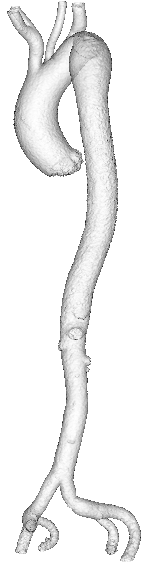
\includegraphics[width=0.7in]{Figures/surface.png}%
\label{fig:SurfaceModel}}
\hfil
\subfloat{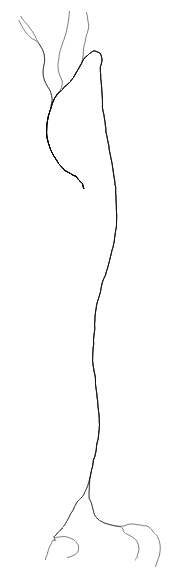
\includegraphics[width=0.9in]{Figures/centerlines.png}%
\label{fig:CenterlinesModel}}
\caption{Visualization models of the aorta: (a) image-based surface model (quantity of consisting polygons: $757,538$); (b) centerlines of the surface model.}%
\label{fig:VisualizationModel}
\end{figure}

\subsection{Discussions}

The computer programs used in this paper were written in C++ based on the Visualization Toolkit, an open source library aims at providing general facilities in the scientific visualization field \cite{Schroeder2000VTK}. %
To depress the unintended affections of the unstructured polygonal surfaces and the noises introduced by the image segmentation, series of steps were introduced in our experiments to extract the centerlines of the surface model of the vasculature. %
During this process, the quantities of the consisting polygons were obviously decreased for the extraction of the largest connected region in the surface model.
Due to the centerlines extraction computation is sensitive and expensive, we subdivided the smoothed surface model based on an improved butterfly scheme.
After this process, the quantities of the consisting polygonal surfaces were increased because of the refinement of the polygons.
With this step, the potential perturbation was further reduced, leading to much less errors which may occur during the computation of the centerlines extraction.
It is noteworthy that the extraction of centerlines for the model surface is an expensive computation both in time and space.
The calculation of the whole aorta (see Fig. \ref{fig:VisualizationModel}) cost nearly eight hours on our desktop machine with dedicated modification on the code to fit the bulky data into the relatively limited memory. %
%The calculation of the whole aorta cost nearly eight hours on our desktop machine with dedicated modification on the code to fit the bulky data into the relatively limited memory. %

\section{Conclusions and Future Work}
%The conclusion goes here.

Centerlines are useful in describing the shape of three dimensional objects.
In implementing the intravascular surgical simulation system, centerlines model of the vasculature will serve as the shape description for the simulation of path planning and navigation of the virtual guidewires/catheters.
In this paper, an automatic approach is designed and validated to extract the centerlines of the image-based patient-specific vasculature model.
The shape analysis presented here lays the foundation for our further research in visualizing the vessels that are closely related to the simulation of PCI procedure.

The connectivity of the polygons in the surface model is firstly checked to find out and remove the redundant polygons that are irrelevant to the actual surface.
Then the resulting surfaces are smoothed at the locations that seems to be uneven in order to prevent these perturbations against the centerlines computation.
After that, the surfaces are subdivided by applying an improved butterfly scheme with the aim of acquiring a more precise surface model.
Finally, the Eikonal equation of the time of arrivals of the embedded Voronoi diagram is computed to obtain the centerlines of the model surface.
Experiments are designed and carried out with the results in demonstrating the effectiveness of the developed approach.

In the future, our research directions are further optimization of the surface model on the one hand, and the visualization of other organs (e.g., heart) and the simulation of the typical phenomena (such as contrast injection, heart beat, etc.) during the procedure on the other. %

%# -*- coding:utf-8 -*-
\chapter{躯干部解剖环境的构建}
\label{chap6}

本章叙述内容:
\begin{enumerate}
  \item 引言
  \item X光影效果
  \item 造影剂注入效果
  \item 心脏搏动效果
  \item 实际验证
  \item 本章小结
\end{enumerate}

\section{引言}

\section{X光影效果}
\label{sec6.2}

\section{造影剂注入效果}

\section{心脏搏动效果}

\section{实际验证}

\section{本章小结}
%# -*- coding:utf-8 -*-
\chapter{组织的物理特性建模及其与手术工具的交互}
\label{chap7}

难点,并且用基于模型的策略来解决姿态评价和
优化的方法往往会具有更好的性能。这里我们以交通场景为研究背景,
讨论基于交通路面场景的运动检测、车辆定位、摄像机标定和模型可. 
%# -*- coding:utf-8 -*-
\chapter{手术流程的状态机模型研究}
\label{chap8}

一般地,一个跟踪预测滤波器的滤波结果好坏取决于两方面的因素:运动模型和滤波器的结构。

本章中提出了一种新的车辆运动模型。
在这个运动模型中考虑了车辆行驶过程中的运动学特性,从而比以前的运动模型更符
合车辆的真实运动。现有的车辆跟踪系统中大多使用了扩展卡尔曼滤波器或者其各种变
体,但是在车辆运动比较复杂时效果不是很好。本章使用了一种改进的扩展卡尔曼滤波器,
加入了一个新的优化目标。实验结果表明,在跟踪车辆运动时,本文中的方法有一定的优点。 
%# -*- coding:utf-8 -*-
\chapter{软件系统的整合}
\label{chap9}

本章叙述内容:
\begin{enumerate}
  \item 引言
  \item 软件系统的设计
  \item 相关的软件库
  \item 工程注记
  \item 本章小结
\end{enumerate}

\section{引言}

\section{软件系统的设计}

\section{相关的软件库}

\section{工程注记}

\section{本章小结}
%# -*- coding:utf-8 -*-
\chapter{总结与展望}
\label{chap10}

自从Marr在其1982年的著名论著\cite{Marr:1982}中提出计算机视觉的理
论框架以来,世界上掀起了研究计算机视觉的高潮,研究者们针对视觉的有关
问题进行了大量的工作,并取得了很大进展。但是,传统的计算机视觉研究
常常认为视觉感知过程的主要任务是物体的三维重建,例如Marr提出的一般
化圆柱模型(generalized
cylinders)\cite{Marr:1982}。从而,二十世纪八九十年代大量关于图像
序列的研究工作主要集中在恢复场景的三维几何结构(如structure from
motion),计算摄像机的运动(ego-motion)和象素的运动信息(例如 光流计算optical
flow)等,很少涉及到图像的高层语义信息。近几年来,对图像序列中的运动
理解越来越受到国际学术界的重视,甚至有人预测动态图像
序列分析和理解将成为21世纪计算机视觉的研究重点。

本文针对路面交通场景动态图像序列的语义理解进行了深入研究,涉及到许多
动态图像语义理解的基本问题,包括摄像机标定、运动检测和分割、目标定位和识别、时空推理、
场景恢复与表示、行为分析和建模、语义理解等等。 


% 附录
%\begin{appendix}
%    \renewcommand{\chaptername}{附录 \Alph{chapter}}
%    \input{appendix/chap01a}
%\end{appendix}
\backmatter %结束章节自动编号

%参考文献
\cleardoublepage
\phantomsection
\bibliographystyle{unsrt}
\addcontentsline{toc}{chapter}{参考文献}
\addtolength{\itemsep}{-2.5 em} % 缩小参考文献间的垂直间距
%%# -*- coding:utf-8 -*- 
%=========================================================================%
%   LaTeX File for phd thesis of Institute of Automation, CAS
%-------------------------------------------------------------------------%
%   Revised by J. G. Lou (jglou@nlpr.ia.ac.cn)
%   参考文献
%-------------------------------------------------------------------------%
\begin{thebibliography}{200}
\bibitem{Marr:1982} D. Marr, Vision-A Computational Investigation into the Human Representation and Processing of Visual Information. W.H. Freeman, 1982.
\bibitem{Witkin:1986} A, Witkin and M. Tenenbaum, ``On perceptual organization'', In \textit{From Pixels to Predicates}, A. Pentland (Ed.). pp. 149-169, 1986.
\bibitem{Buxton:2000} H. Buxton and A. Mukerjee, ``Conceptualizing Images'', \textit{Image and Vision Computing}, Vol. 18, pp. 79, 2000.
\bibitem{Mubarak:2002} Mubarak Shah, ``Guest Introduction: The Changing Shape of Computer Vision in the Twenty-First Century'', \textit{International Journal of Computer Vision}, Vol. 50(2), pp. 103-110, 2002.
\bibitem{Shi:1994} J. Shi and C. Tomasi, “Good Features to Track”, Proc.of IEEE Int. Conf. on Computer Vision and Pattern Recognition (CVPR'94), pp. 593 -- 600, 1994.
\bibitem{Malik:1997} J. Malik and S. Russell, “Traffic Surveillance and Detection Technology Development: New Sensor Technology Final Report”, Research Report UCB-ITS-PRR-97-6, California PATH Program, 1997.
\bibitem{Peter:1990} K. Peter, Karmann and A. Brandt, ``Moving Object Recognition Using an Adaptive Background Memory”, in V Cappellini, editor, Time-Varying Image Processing and Moving Object Recognition, Elsevier, Amsterdam, The Netherlands, 1990.
\bibitem{Blake:1997} A. Blake and M. Isard, “Active Contours: The Application of Techniques from Graphics, Vision, Control Theory and Statistics to Visual Tracking of Shapes in Motion'', Springer, 1997.
\bibitem{Kojima:2000} A. Kojima, M. Izumi, et al. ``Generating Natural Language Description of Human Behavior from Video Images'', In Proceeding of International Conference on Pattern Recognition, pp. 728-731, 2000.
\bibitem{Kojima:2002} A. Kojima, T. Tamura, ``Natural Language Description of Human Activities from Video ImagesBased on Concept Hierarchy of Actions'', International Journal of Computer Vision 50(2), 171--184, 2002.
\bibitem{Kollnig:1994} H. Kollnig, H.H. Nagel and M. Otte, ``Association of Motion Verbs with Vehicle Movements Extracted from Dense Optical Flow Fields'', In Proceedings of 3rd European Conference on Computer Vision '94, pp. 338-347, 1994.
\bibitem{Haag:2000} M. Haag, H. H. Nagel, ``Incremental recognition of traffic situations from video image sequences'', Image and Vision Computing, Vol. 18, pp. 137-153, 2000.
\bibitem{Herzog:1995} G. Herzog, ``From Visual Input to Verbal Output in the Visual Translator'', In: R.~K. Srihari (ed.), Proc. of the AAAI Fall Symposium on Computational Models for Integrating Language and Vision, MIT, Cambridge, MA, Nov. 10, 1995.
\bibitem{Gerd:1995} Gerd Herzog, Karl Rohr, “Integrating Vision and Language Towards Automatic Description of Human Movements'', In Proceedings of the 19$^{th}$ Annual German Conference on Artificial Intelligence, KI-95, 1995.
\bibitem{Artificial:1994} Artificial Intelligence Review Journal, 8, Special Volume on the Integration of Natural Language and Vision Processing, 1994.
\bibitem{The:1995} The AAAI Fall Symposium on Computational Models for Integrating Language and Vision, Cambridge, MIT, 1995.
\bibitem{VSAM:1} VSAM Homepage: \href{http://www.cs.cmu.edu/~vsam}{http://www.cs.cmu.edu/$\sim $vsam}.
\bibitem{Roberts:1} L.G. Roberts, ``Machine Perception of Three-Dimensional Solids'', Optical and Electro-Optical Information Processing, J.P. Tippet et al. Eds. Pp. 159-197, Cambridge, MIT Press.
\bibitem{Marr:1980} D. Marr and E. Hidreth, ``Theory of edge detection'', In Proc. R. Soc. Lond., vol. B-207, pp. 187-217, 1980.
\bibitem{Masongde:1998} 马颂德,张正友,计算机视觉――计算理论与算法基础,科学出版社,1998.
\bibitem{human:1} http://human-brain.org/vision.html
\bibitem{Cedras:1995} C. Cedras and M. Shah, ``Motion based recognition: A survey'', Image and Vision Computing, Vol. 13(2), pp. 129-155, 1995.
\bibitem{Fisher:1994} R.B. Fisher, ``Is Computer Vision Still AI'', AI Magazine, Jun. 1994.
\bibitem{Lowe:1992} D. G. Lowe, ``Robust Model-Based Motion Tracking Through the Integration of Search and Estimation'', International Journal of Computer Vision, Vol. 8, No. 2, pp. 113-122, 1992.
\bibitem{Stauffer:1999} C. Stauffer and W. E . L. Grimson, ``Adaptive Background Mixture Models for Real-time Tracking'', Proc. of IEEE Int. Conf. of Computer Vision and Pattern Recognition (CVPR'99), Vol.2, pages 246-252, 1999.
\bibitem{Peter:1991} K. Peter, Karmann and A. Brandt, ``Moving Object Recognition Using an Adaptive Background Memory”, in V Cappellini, editor, Time-Varying Image Processing and Moving Object Recognition, Elsevier, Amsterdam, The Netherlands, 1990.
\bibitem{Sun:2000} H. Z. Sun, T. Feng and T. N. Tan, ``Robust extraction of moving objects from video sequences'', In Proceedings of the Fourth Asian Conference on Computer Vision, Vol. 2, pp. 961-963 , Jan. 2000.
\bibitem{Ridder:1994} C. Ridder, O. Munkelt and H. Kirchner, ``Adaptive Background Estimation and Foreground Detection using Kalman-Filtering'', International Conference on Recent Advances in Mechatronics, UNESCO Chair on Mechatronics, pp. 193-199, 1994.
\bibitem{Huwer:2000} S. Huwer, H. Niemann, ``Adaptive Change Detection for Real-time Surveillance Applications'', Workshop on Visual Surveillance in ECCV2000, 2000.
\bibitem{Gevers:1998} T. Gevers, A. W. M. Smeulders and H. Stokman, ``Photometric Invariant Region Detection'', In Proceeding of Britsh Machine Vision Conference, pp. 659-669, 1998.
\bibitem{Wren:1997} C. Wren, A. Azarbayejani, T. Darrell and A. Pentland, ``Pfinder: Real-Time Tracking of the Human Body”, IEEE Transaction on Pattern Analysis and Machine Intelligence, Vol. 19, no. 7, pp. 780-785, 1997.
\bibitem{Stauder:1997} J. Stauder, ``Segmentation of Moving Objects in Presence of Moving Shadows'', In Proceeding of VLBV 97, Linkoeping, Sweden, July, 1997.
\bibitem{Cavallaro:2001} A. Cavallaro and T. Ebrahimi, ``Change Detection Based on Color Edges'', In Proceeding of IEEE International Symposium on Circuits and Systems, Sydney (Australia), May 2001.
\bibitem{Ivanov:1998} Y. Ivanov, A. Bobick and J. Liu, ``Fast Lighting Independent Background Subtraction'', In Proceeding of the IEEE Workshop of Visual Surveillance, pp. 49-55, Bomgay, India, Jan. 1998.
\bibitem{Eveland:1998} C. Eveland, K. Konolige and R. C. Bolles, ``Background Modeling for Segmentation of Video-Rate Stereo Sequences'', In Proceeding of IEEE Conference on Computer Vision and Pattern Recognition, pp. 266-271, Jun. 1998.
\bibitem{Gordon:1999} G. Gordon, T. Darrell, M. Harville, J. Woodfill, ``Background estimation and removal based on range and color'', International Conference of Computer Vision and Pattern Recognition, 1999.
\bibitem{Daniel:2000} Daniel Toth, Til Aach, and Volker Metzler, ``Illumination--Invariant Change Detection”, 4$^{th}$ IEEE Southwest Symposium on Image Analysis and Interpretation, April, 2000.
\bibitem{Jianguang:2002} Jianguang Lou, Hao Yang, Weiming Hu, Tieniu Tan, ``An Illumination Invariant Change Detection Algorithm'', the 5$^{th}$ Asia Conference on Computer Vision, Australia, 2002.
\bibitem{Aach:1993} T. Aach, A. Kaup and R. Mester, ``Change Detection in Image Sequences Using Gibbs Random Fields: A Bayesian Approach'', In Proceeding of IEEE International Workshop on Intelligent Signal Processing and Communications Systems, Sendai, Japan, pp. 376-381, Oct. 1993.
\bibitem{Jens:2000} Jens Rittscher Jien Kato Sebastien Joga and Andrew Blake, ``A Probabilistic Background Model for Tracking”, In Proceeding of European Conference on Computer Vision, 2000.
\bibitem{Paragios:1999} N. Paragios and G. Tziritas, ``Adaptive Detection and Localization of Moving Objects in Image Sequences,'' Signal Processing: Image Communication, Vol. 14, pp.277--296, 1999.
\bibitem{Paragios:1996} N. Paragios, P. Perez, G. Tziritas, C. Labit, and P. Bouthemy, “Adaptive detection of moving objects using multiscale techniques”, \textit{IEEE Intern. Conf. on Image Processing}, Switzerland, pp. 525-528, 1996.
\bibitem{Rasmussen:1} C. Rasmussen and G. D. Hager, ``Probabilistic Data Association Methods for Tracking Complex Visual Objects'', IEEE Transactions on Pattern Analysis and Machine Intelligence, Vol. 23, No.6, June
2001.
\bibitem{JPL:1997} JPL, Traffic Surveillance and Detection Technology Development, Sensor Development Final Report, Jet Propulsion Laboratory Publication No. 97-10, 1997.
\bibitem{Malik:1} J. Malik, S. Russell, J. Weber, T. Huang and D. Koller, ``A Machine Vision Based Surveillance System for Californaia Roads'', PATH project MOU-83 Final Report, University of California.
\bibitem{Kass:1987} M.Kass, A. Witkin and D. Terzopoulos, ``Snakes: Active Contour Models'', International Journal of Computer Vision, vol.1, pp. 321-331, 1987.
\bibitem{Andrew:1998} Andrew Blake and Michael Isard, “Active Contours”, Springer-Verlag, 1998.
\bibitem{Caselles:1997} V. Caselles, R. Kimmel and G. Sapiro, “Geodesic Active Contours” International Journal of Computer Vision, pp. 22:61-79, 1997.
\bibitem{Kichenassamy:1995} S. Kichenassamy, A. Kumar, P. Olver, A. Tannenbaum and A. Yezzi, ``Gradient Flows and Geometric Active Contour Models”, International Conference of Computer Vision, pp. 810-815, Boston, USA, 1995.
\bibitem{Malladi:1991} R. Malladi, J. Sethian and B. Vemuri, “Shape Modeling with Front Propagation: A Level Set Approach”, IEEE Conference on Computer Vision and Pattern Recognition, pp. 337-343, 1991.
\bibitem{Nikos:2002} Nikos Paragios and Rachid Deriche, “Geodesic Active Regions: A new Paradigm to deal with frame partition Problems in Computer vision”, Journal of Visual Communication and Image Representation, pp. 266-280, 2002.
\bibitem{Nikos:2000} Nikos Paragios and Rachid Deriche, “Geodesic Active Contours and Level Sets for the Detection and Tracking of Moving Objects”, IEEE Transactions on Pattern Analysis and Machine Intelligence, vol. 22, pp. 266-280, 2000.
\bibitem{Jitendra:1997} Jitendra Malik and Stuart Russell, ``Traffic Surveillance and Detection Technology Development: New Traffic Sensor Technology”, California PATH Research Final Report, UCB-ITS-PRR-97-6, University of California, Berkeley, 1997.
\bibitem{Koller:1994} D. Koller, J. Weber, T. Huang,J. Malik, G. Ogasawara, B. Rao, and S. Russell, ``Towards Robust Automatic Traffic Scene Analysis in Real-Time'', In Proceeding of IAPR International Conference on Pattern Recognition (ICPR94), pp. 126-131, 1994.
\bibitem{Malik:2} J. Malik, S. Russell, J. Weber, T. Huang and D. Koller, ``A Machine Vision Based Surveillance System for Californaia Roads'', PATH project MOU-83 Final Report, University of California.
\bibitem{Fan:1989} Fan, T. J., Medioni, G., and Nevatia, ``Recognizing 3-D Objects Using Surface Descriptions'', IEEE Transaction on Pattern Analysis and Machine Intelligence, Vol.11, pp. 1140-1157, 1989.
\bibitem{Beymer:1998} D. Beymer, P. Mclauchlan, and J. Malik, ``A Real-time Computer Vision System for Vehicle Tracking and Traffic Surveillance'', Submitted for publication in Transportation Research-C, 1998.
\bibitem{Malik:1996} J. Malik, S. Rusell, ``Traffic Surveillance and Detection Technolodgy Development (New Traffic Sensor Technology)'', Final Report, University of California, Berkeley, 1996.
\bibitem{Chachich:1} Chachich, A. Pau, A, Barber, et al., ``Traffic Sensor Using a Color Vision Method, Transportation Sensors and Controls: Collision Avoidance, Traffic Management, and ITS'', SPIE Proceedings, Vol. 2902, pp. 156-165.
\bibitem{Bernt:2000} Bernt Schiele, ``Vodel-Free Tracking of Cars and People Based on Color Regions'', Proceeding of 1st IEEE International Workshop on Performance Evaluation of Tracking and Surveillance(PETS'2000), Grenoble, France, pp. 61-71, 2000.
\bibitem{Tan:2000} T. N. Tan and K. D. Baker, Efficient Image Gradient Based Vehicle Localization, IEEE Transaction on Image Processing, vol.9(8), pp. 1343-1356, 2000.
\bibitem{Tan:1998} T. N. Tan, G. D. Sullivan and K. D. Baker, Model-Based Localization and Recognition of Road Vehicles, International Journal of Computer Vision, vol.27(1), pp. 5-25, 1998.
\bibitem{Sullivan:1992} G. D. Sullivan, Visual Interpretation of Known Objects in Constrained Scenes, Phil. Trans. Royal Society (B) 337, pp. 361-370, 1992.
\bibitem{Worrall:1991} A. D. Worrall, R. F. Marslin, G. D. Sullivan, K. D. Baker, Model-Based Tracking, Proc. British Machine Vision Conference (BMVC91), pp. 310-318, 1991.
\bibitem{Koller:1993} D. Koller, K. Daniilidis and H.-H. Nagel, Model-Based Object Tracking in Monocular Image Sequences of Road Traffic Scenes, International Journal of Computer Vision, vol.10(3), pp. 257-281, 1993.
\bibitem{Kollnig:1997} H. Kollnig and H-H. Nagel, 3D Pose Estimation by Directly Matching Polyhedral Models to Gray Value Gradients, International Journal of Computer Vision, vol.23(3), pp. 283-302, 1997.
\bibitem{Haag:1999} M. Haag and H-H. Nagel, Combination of Edge Element and Optical Flow Estimates for 3D-Model-Based Vehicle Tracking in Traffic Image Sequences, International Journal of Computer Vision, vol.35(3), pp. 295-319, 1999.
\bibitem{Haag:1997} M. Haag, Th. Frank, H. Kollnig and H.-H. Nagel, ``Influence of an Explicitly Modeled 3D Scene on the Tracking of Partially Occluded Vehicles'', Computer Vision and Image Understanding, Vol. 65, No. 2, pp. 206-225, 1997.
\bibitem{Jacobs:1997} D. W. Jacobs, ``Matching 3-D Models to 2-D Images'', International Journal of Computer Vision, Vol. 21, No. 1, pp. 123-153, 1997.
\bibitem{Lowe:1993} D. G. Lowe, ``Robust Model-Based Motion Tracking Through the Integration of Search and Estimation'', International Journal of Computer Vision, Vol. 8, No. 2, pp. 113-122, 1992.
\bibitem{Daucher:1993} N. Daucher, M. Dhome, J. T. Lapreste and G. Rives, ``Modeled Object Pose Estimation and Tracking by Monocular Vision'', In British Machine Vision Conference, BMVC'93, pp. 249-258, UK, 1993.
\bibitem{Gennery:1992} D. B. Gennery, ``Visual Tracking of Known three-dimensional Objects'', International Journal of Computer Vision, Vol. 7(3), pp.243-270, 1992.
\bibitem{Brisdon:1987} K. Brisdon, Evaluation and Verification of Model Instances, \textit{Proc. Alvey Vision Conference}, pp. 33-37, 1987.
\bibitem{Sullivan:1993} G. D. Sullivan, A. D. Worrall, T. N. Tan, et al., Model Based Vision in VIEWS, Report of EP2152: VIEWS, Reading University, UK, 1993.
\bibitem{Pece:2000} A. E. C. Pece, A. D. Worrall, Tracking without Feature Detection, Pro. 1st IEEE International Workshop on Performance Evaluation of Tracking and Surveillance(PETS'2000), Grenoble, France, pp. 29-37, 2000.
\bibitem{Pece:1998} A. E. C. Pece, A. D. Worrall, A Statistically-based Newton Method for Pose Refinement. Image and Vision Computing, Vol. 16, pp. 541-544, 1998.
\bibitem{Lowe:1994} D. G. Lowe, ``Robust Model-Based Motion Tracking Through the Integration of Search and Estimation'', International Journal of Computer Vision, Vol. 8, No. 2, pp. 113-122, 1992.
\bibitem{Yang:2001} H. Yang, J. G. Lou, H. Z. Sun, W. M. Hu and T. N. Tan, ``Efficient and Robust Vehicle Localization'', In Proceeding of International Conference on Image Processing, pp. 355-358, 2001.
\bibitem{Kalman:1960} Kalman, R. E. ``A New Approach to Linear Filtering and Prediction Problem'', Journal of Basic Engineering, vol. 82, pp. 35-45, 1960.
\bibitem{Cox:1994} I. J. Cox and S. L. Hingorani, ``An Efficient Implementation and Evaluation of Reid's Multiple Hypothesis Tracking Algorithm for Visual Tracking'', In Proceeding of International Conference on Pattern Recognition, pp. 437-442, 1994.
\bibitem{Koller:1995} D. Koller, J. Weber and J. Malik, ``Robust Multiple Car Tracking with Occlusion Reasoning'', In Proceeding of the 3$^{rd}$ European Conference on Computer Vision, pp. 186-196, Stockholm, 1994.
\bibitem{Haritaoglu:1998} I. Haritaoglu, D. Harwood and L. S. Davis, ``W4: Who? When? Where? What? A Real Time System for Detecting and Tracking People'', In Proceeding of 3$^{rd}$ International Conference on Face and Gesture Recognition, pp. 222-227, Japan, 1998.
\bibitem{Blake:1995} A. Blake, M. Isanc and D. Reynard, ``Learning to Track the Visual Motion of Contours'', Artificial Intelligence, vol. 78, pp. 101-133, 1995.
\bibitem{Rosales:1998} R. Rosales and S. Sclaroff, ``Improved Tracking of Multiple Humans with Trajectory Prediction and Occlusion Modeling'', CVPR Workshop on the Interpretation of Visual Motion, 1998.
\bibitem{Bregler:1997} C. Bregler, ``Learning and Recognition Human Dynamics in Video Sequences'', In Proceeding of International Conference on Computer Vision and Pattern Recognition, pp. 568-574, 1997.
\bibitem{Robert:1999} T. C. Robert, J. L. Alan and K. Takeo, ``A System for Video Surveillance and Monitoring'', In Proceeding of the American Nuclear Society Eighth International Topical Meeting on Robotics and Remote Systems, Apr. 1999.
\bibitem{Koller:1996} D. Koller, K. Daniilidis and H. H. Nagel, ``Model-Based Object Tracking in Monocular Image Sequences of Road Traffic Scenes'', Journal of Computer Vision, Vol. 10, No. 3, pp. 257-281, 1993.
\bibitem{Liu:1998} J. S. Liu and R. Chen, ``Sequential Monte Carlo Methods for Dynamical Systems'', Journal of American Statist Association, vol. 93, pp. 1032-1044, 1998.
\bibitem{Gordon:1997} N. J. Gordon, ``A Hybrid Bootstrap Filter for Target Tracking in Clutter'', IEEE Transaction on Aerospace and Electronic Systems, vol. 33, no. 1, pp. 353-358, 1997.
\bibitem{Isard:1996} M. Isard and A. Blake, ``Contour Tracking by Stochastic Propagation of Conditional Density'', In Proceeding of Europe Conference on Computer Vision, pp. 343-356, 1996.
\bibitem{Maybank:1996} S. J. Maybank, A. D. Worrall and G. D. Sullivan, ``A Filter for Visual Tracking Based on A Stochastic Model for Driver Behaviour'', In Proceeding of the Fourth European Conference on Computer Vision, vol.2, pp. 540-549, UK, Apr. 1996.
\bibitem{Maybank:1997} S. J. Maybank, A. D. Worrall and G. D. Sullivan, ``Filter for Car Tracking Based on Acceleration and Steering Angle'', In Proceeding of British Machine Vision Conference, pp. 615-624, Sep. 1996.
\bibitem{John:2001} John K. Tsotsos, ``Motion Understanding: Task-Directed Attention and Representations that Link Perception with Action'', International Journal of Computer Vision, vol. 45(3), pp. 265-280, 2001.
\bibitem{Badler:1975} N. I. Badler, ``Temporal scene analysis: Conceptual descriptions of objects movements'', Ph.D. Thesis, Department of Computer Science, University of Toronto, 1975.
\bibitem{Tsotsos:1980} Tsotsos,J., Mylopoulos,J., Covvey,H.D., Zucker,S.W., "A Framework for Visual Motion Understanding", IEEE Pattern Analysis and Machine Intelligence, "Special Issue on Computer Analysis of Time-Varying Imagery", p563 -- 573, Nov. 1980.
\bibitem{Dance:1993} S. Dance and T. Caelli, ``On the symbolic interpretation of traffic scenes'', In Proceedings of the Asian Conference on Computer Vision (ACCV93), pp 798-801, Osaka, 1993.
\bibitem{Dance:1994} S. Dance and T. Caelli, “A Symbolic Object Oriented Picture Inter- pretation Network: SOO-PIN”, Advances in Structural and Syntactic Pattern Recognition, Proceedings of the International Workshop, Horst Bunke, pp 530-541, Bern, 1993.
\bibitem{Dance:1995} S. Dance, T. Caelli, and Z-Q Liu, “An Architecture for A Traffic Scene Interpretation System”, Technical Report No. 94/12, pp. 1-43, Department of Computer Science, University of Melbourne, 1994.
\bibitem{Liu:2001} Z. Q. Liu, L. T. Bruton, J. C. Bezdek, J. M. Keller, S. Dance, M. R. Bartley and C. Zhang,``Dynamic Image Sequence Analysis Using Fuzzy Measures'', IEEE TRANSACTIONS ON SYSTEMS, MAN, AND CYBERNETICS---PART B: CYBERNETICS, VOL. 31, NO. 4, pp. 557-572, Aug. 2001.
\bibitem{Dance:1996} S. Dance and Z.-Q. Liu, ``Fuzzy belief and scene interpretation'', in T. Huang and S. Negadharipour, editors, Proceedings of the 1995 IEEE International Conference on Computer Vision, Florida, 1995.
\bibitem{Dance:1997} S. Dance and Z. Q. Liu, ``High Level Scene Interpretation using Fuzzy Belief'', In Proceeding of ICSC, pp. 258-265, 1995.
\bibitem{Remagnino:1998} P. Remagnino, T. Tan and K. Baker, “Agent Orientated Annotation in Model Based Visual Surveillance”, In Proceeding of IEEE International Conference on Computer Vision, pp857-862, 1998.
\bibitem{Huang:1994} T. Huang, D. Koller, J. Malik, G. Ogasawara, B. Rao, S. Russell and J. Weber, ``Automatic Symbolic Traffic Scene Analysis Using Belief Networks'', In Proceeding of 12th National Conferece in AI, pp. 966---972, 1994.
\bibitem{Sumpter:2000} N. Sumpter and A. Bulpitt, ``Learning Spatio-temporal Patterns for Predicting Object Behaviour'', Image and Vision Computing, vol.18, no. 1, pp. 697-704, 2000.
\bibitem{Howell:1997} A. J. Howell and H. Buxton, ``Recognising Simple Behaviours using Time-Delay RBF Networks'', Neural Processing Letters (5), pp.97-105, 1997.
\bibitem{Fernyhough:2000} J. Fernyhough, A.G. Cohn and D.C. Hogg, ``Constructing qualitative event models automatically from video input'', Image and Vision Computing, vol.18(1), pp. 81-103, 2000.
\bibitem{Wada:2000} T. Wada, T. Matsuyama, ``Multiobject Behavior Recognition by Event Driven Selective Attention Method'', IEEE Trans. On Pattern Analysis and Machine Intelligence, vol.22(8), pp.873-887, 2000.
\bibitem{Galata:1999} A. Galata, N. Johnson and D. Hogg, ``Learning Structured Behaviour Models Using Variable Length Markov Models”, IEEE International Workshop on Modelling People, Corfu, Greece, Sep. 1999.
\bibitem{Yamata:1992} J. Yamata, J. Ohya and K. Ishii, ``Recognizing Human Action in Time-Sequential Images Using Hidden Markov Model'', Proceeding of International Conference on Computer Vision and Pattern Recognition, pp. 664-665, 1992.
\bibitem{Brand:1996} M. Brand, N. Oliver and A. Pentland, “Coupled hidden Markov models for complex action recognition” , Learning and Common Sense Technical Report 407, MIT Media Lab Perceptual Computing,1996.
\bibitem{Johnson:1998} N. Johnson, “Learning Object Behaviour Models”, Ph.D. thesis, The University of Leeds, Sep. 1998.
\bibitem{Bobick:1995} A. Bobick and A. Wilson, ``A state-based technique for the summarization and recognition of gesture'', in Proc. of International Conference on Computer Vision, pp. 382-388, Cambridge, 1995.
\bibitem{Takahashi:1994} K. Takahashi, S. Seki, et al, ``Recognition of dexterous manipulations from time varying images'', in Proc. of IEEE Workshop on Motion of Non-Rigid and Articulated Objects, pp. 23-28, Austin, 1994.
\bibitem{Bobick:1996} A. F. Bobick and J. Davis, ``Real-time recognition of activity using temporal templates'', in Proc. of IEEE CS Workshop on Applications of Computer Vision, pp. 39-42, 1996.
\bibitem{Changya:2001} 昌娅, 胡卫明, 谭铁牛. ``交通视觉监控系统中的三维车辆线框模型可视化算法'',工程图学学报增刊,28~33,2001.
\bibitem{Wang:1991} L. L. Wang, W. H. Tsai, ``Camera Calibration by Vanishing Lines for 3D Computer Vision'', IEEE Trans. on Pattern Recognition and Machine Intelligence, vol. 13(3), pp. 370-376, 1991.
\bibitem{Huang:1999}J. B. Huang, Z. Chen , J. Y. Lin, ``A Study On The Dual Vanishing Point Property'', Pattern Recognition, vol. 32(12), pp. 2029-2039,1999.
\bibitem{Caprile:1990} B. Caprile, and V. Torre, ``Using Vanishing Points for Camera Calibration'', International Journal of Computer Vision, vol. 4(2), pp. 127-140,1990.
\bibitem{Zhang:2000} Z. Zhang, ``A Flexible New Technique for Camera Calibration'', IEEE Transaction on Pattern Analysis and Machine Intelligence, vol. 22(11), pp. 1330-1334,2000.
\bibitem{Self:1996} S. D. Ma, ``A Self-calibration Technique for Active Vision System'', IEEE Transaction on Robot Automat, vol. 12(1), pp. 114-120,1996.
\bibitem{Basu:1993} A. Basu, ``Active Calibration: Alternative Strategy and Analysis'', In: Proceeding of IEEE Conference on Computer Vision and Pattern Recognition, New York, 495-500, 1993.
\bibitem{Sturm:1999} P. F. Sturm, S. J. Maybank, ``On Plane-based Camera Calibration: A General Algorithm, Singularities, Applications'', In: Proceeding of IEEE Conference on Computer Vision and Pattern Recognition, Fort Collins, 432-437, 1999.
\bibitem{Gevers:1999} T. Gevers, A. W. M. Smeulders and H. Stokman, ``Photometric Invariant Region Detection'', In Proceeding of British Machine Vision Conference (BMVC), pp. 659-669, 1998.
\bibitem{Liuqf:2002} Q. F. Liu, J. G. Lou, Weiming Hu, Tieniu Tan, "Comparison of model-based pose evaluation algorithm in traffic scenes", the 2nd International Conference on Image and Graphics, Hefei, 2002.
\bibitem{Liuqf:2003} Q. F. Liu, J. G. Lou, T. N. Tan, W. M. Hu, "POSE EVALUATION BASED ON BAYESIAN CLASSIFICATION ERROR", submitted to ICIP2003.
\bibitem{Lihezhou:1985} 邹理和、吴兆熊,数字信号处理,国防工业出版社,1985年.
\bibitem{Zhou:1991} D. H. Zhou, Y. G. Xi and Z. J. Zhang, A Nonlinear Adaptive Fault Detection Filter, International Journal of System Science, vol. 22 (12), pp. 2563-2571, 1991.
\bibitem{Bobick:1997} A. F. Bobick, "Movement, Activity, and Action: The Role of Knowledge in the Perception of Motion", The Royal Society Workshop on Knowledge-based vision in mam and Machine, London, Feb. 1997.
\bibitem{Nagel:1988} H. H. Nagel, "From image sequences towards conceptual descriptions", Image and Vision Computing, Vol.16, pp. 73-111, 1997.
\bibitem{Neumann:1989} B. Neumann, "Natural Language Description of Time-Varying Scenes", In: D. L. Waltz(ed.), Semantic Structures: Advances in Natural Language Processing, pp. 167-207, Hillsdale, NJ: Lawrence Erlbaum, 1989.
\bibitem{Gardenfors:1991} P. G\"{a}rdenfors, "Conceptual sapces as a framework for cognitive semantics", Proceedings of the Second International Colloquium on Cognitive Science, 1991.
\bibitem{Gardenfors:1997} P. G\"{a}rdenfors, "Meanings as Conceptual Structures", In Mindscapes: Philosophy, Science, and the Mind, ed. by M. Carrier, Pittsburgh University Press, Pittsburgh, pp. 61-86, 1997.
\bibitem{Aristotle:0} Aristotle, "On Intepretation", translated by E. M. Edghill, http://www.non-contradiction.com.
\bibitem{Rohini:1995} Rohini K. Srihari, "Computational models for integrating liguistic and visual information: A survey", Artificial Intelligence Review, vol. 8(5), pp. 349-369, 1995.
\bibitem{Kosslyn:1990} S. M. Kosslyn, "Mental Imagery", In Daniel N. Osherson et al., editor, \textit{Visual Cognitive and Action}, pp. 73-97, MIT Press, Cambridge Mass, 1990.
\bibitem{Chella:1997} A. Chella, M. Frixione and S. Gaglio, "A Cognitive Arichitecture for Artificial Vision", Artificial Intelligence, vol. 89, pp. 73-111, 1997.
\bibitem{Gardenfors:1993} P. G\"{a}rdenfors, "Induction and the evolution of conceptual spaces", in Charles Peirce and the Philosophy of Science: Papers from the Harvard Sesquicentennial Conference, ed. by E.C. Moore, University of Alabama Press, pp. 72-88, 1993.
\bibitem{Fraile:1998} R. Fraile and S. J. Maybank, "Vehile Trajectory Approximation and Classification", In Proceedings of British Machine Vision Conference, 1998.
\bibitem{Johnson:1996} N. Johnson and D. C. Hogg, "Learning the Distribution of Object Trajectories for Event Recognition", Image and Vision Computing, vol. 14, pp. 609-615, 1996.
\bibitem{Stauffer:2000} C. Stauffer and E. Grimson, "Learning Patterns of Activity Using Real-Time Tracking", IEEE Transaction on Pattern Analysis and Machine Intelligence, vol.22, no.8, pp. 747-757, 2000.
\bibitem{Johnson:1987} M. Johnson, "The Body in the Mind: The Bodily Basis of Reason and Imagination", Chicago: The University of Chicago Press, 1987.
\bibitem{Stalnaker:1981} R. Stalnaker, "Antiessentialism", Midwest Studies of Philosophy 4: 343-355, 1981.
\bibitem{Gardenfors:1991b} P. G\"{a}rdenfors, "Frameworks for properties: Possible worlds vs. conceptual spaces", Language, Knowledge and Intentionality, Acta Philosophica Fennica, vol. 49, pp. 383-407, 1991.
\bibitem{Thibadeau:1994} R. H. Thibadeau, "Artificial Perception of Actions", Gognitive Science, Feb. 1994. http://www.ri.cmu.edu/pubs/pub\_2960.html
\bibitem{Allen:1983} J. F. Allen, "Maintaining Knowledge about Temporal Intervals", Communications of ACM, Vol. 26, No. 11, pp. 832-843, 1983.
\bibitem{Allen:1994} J. F. Allen and G. Ferguson, "Actions and Events in Interval Temporal Logic", Journal of Logic and Computation, Vol.4(5), pp. 531-579, 1994.
\bibitem{Yamato:1992} J. Yamato, J. Ohya, and K. Ishii. "Recognizing Human Action in Time-Sequential Images Using Hidden Markov Model", In Proceedings of International Conference on Computer Vision and Pattern Recognition, pp. 379-385. 1992.
\bibitem{Wilson:1995} A. Wilson and A. F. Bobick. "Learning Visual Behavior for Gesture Analysis", Proc. of the IEEE-PAMI International Symposium on Computer Vision, Coral Gables, Florida, pp. 229-234. November. 1995.
\bibitem{Stein:1994} L. A. Stein and L. Morgenstern. "Motivated Action Theory: a Formal Theory of Causal Reasoning", Artificial Intelligence, vol. 71, pp. 1-42. 1994.
\bibitem{Leith:1997}  M. F. Leith and R. J. Cunningham, "Representing and Reasoning with Events from Natural Language", in Gabbay et al. (eds) Qualitative and Quantitative Practical Reasoning (EQUARU/FAPR 97, Bad Honnef), Springer LNAI 1244, 1997.
\bibitem{Xiaoling:1994} 左孝凌,李为鑑,刘永才,“离散数学”,上海科学技术文献出版社,1982年第一版,1994第17次印刷.
\bibitem{Wenxiu:1996} 张文修,梁  怡,“不确定性推理原理”,西安交通大学出版社,1996.
\bibitem{Talavera:2001} Luis  Talavera, Javier  Béjar, "Generality-Based Conceptual Clustering with Probabilistic Concepts", IEEE Transaction on Pattern Analysis and Machine Intelligence, Vol. 23, No. 2, pp. 196-206, 2001.
\bibitem{Kogut:2002} G. Kogut, M. Trivedi, "A Wide Area Tracking System for Vision Sensor Networks," In the 9th World Congress on Intelligent Transport Systems, Chicalgo, Oct. 2002.
\bibitem{Lee:1995} J. W. Lee, M. S. Kim and I. S. Kweon, "A Kalman Filter Based Visual Tracking Algorithm for An Object Moving in 3D", Proc. of the Int'l Conf. on Intelligent Robots and Systems, Aug. 1995.
\bibitem{Costa:2000}M.S. Costa and L.G. Shapiro, "3D Object Recognition and Pose With Relational Indexing", Computer Vision and Image Understanding, vol. 79, no. 3, pp. 364-407, 2000.
\end{thebibliography}

%%# -*- coding:utf-8 -*-
%=========================================================================%
%   LaTeX File for phd thesis of Institute of Automation, CAS
%-------------------------------------------------------------------------%

%%%%%%%%%%%%%%%%%%%%%%%%%%%%%%%%%%%%%%%%%%%%%%%%%%%%%%%%%%%%%%%
%文件头部定义
%%%%%%%%%%%%%%%%%%%%%%%%%%%%%
\documentclass [12pt,a4paper,twoside] {book}
%\documentclass [12pt,a4paper,openany,twoside,draft] {book}
%============================ 引用的宏包 ==================================%
%# -*- coding:utf-8 -*-
%=========================================================================%
%   LaTeX File for phd thesis of Institute of Automation, CAS
%-------------------------------------------------------------------------%
%   张兆翔将原来的dvipdf改为dvipdfm宏包,可使用latex + dvipdf自动生成索引
%-------------------------------------------------------------------------%
%   Revised by J. G. Lou (jglou@nlpr.ia.ac.cn)
%-------------------------------------------------------------------------%
%=========================================================================%
%                          引用的宏包和相应的定义
%=========================================================================%

%============================ 中文支持宏包 ==============================%
% \usepackage{CJK}
\usepackage{CJKutf8}

%====================== 图形和超链接支持宏包 ========================%
% 图形支持宏包 为了使用PDFLaTeX需要作相应判断
% hyperref
% 可以在转换为pdf文件时自动加入索引, dvi2ps 加入-z 参数
% 为了支持pdftex 使用不同的宏包选项
\ifx\pdfoutput\undefined
\usepackage[dvips]{graphicx}
\usepackage[dvipdfm,
            pagebackref,
            %backref,
            unicode=true,
            % CJKbookmarks=true,
            bookmarksnumbered=true
            % bookmarksopen=false,
            ]{hyperref}
\else
\usepackage[dvipdfm,
            pagebackref,
            %backref,
            unicode=true,
            % CJKbookmarks=true,
            bookmarksnumbered=true
            ]{hyperref}
\usepackage[pdftex]{graphicx}
\fi


% \usepackage{ccmap}


\usepackage{color}      % 支持彩色
\usepackage{subfigure}  % 支持子图
\usepackage{floatflt}   % 图文混排用宏包
\usepackage{rotating}   % 图形和表格的控制
\usepackage{flafter}    % 因为图形可浮动到当前页的顶部,所以它可能会出现
                        % 在它所在文本的前面. 要防止这种情况,可使用 flafter
                        % 宏包

\usepackage[below]{placeins}    %浮动图形控制宏包
                                %允许上一个section的浮动图形出现在下一个
                                %section的开始部分该宏包提供处理浮动对象
                                %的 \FloatBarrier 命令,使所有未处理的浮动
                                %图形立即被处理
%\usepackage{endfloat}  %可将浮动对象放置到文件的最后
%\usepackage{overpic}   %将LaTeX对象放置在图上
%\usepackage{pstricks}  %Postscript macrosfor Generic TeX(我没用过,据说很强)
\usepackage{bez123}

%============================表格支持宏包=================================%
\usepackage{rotating}   % 用法 \begin{sidewaystable}....\end{sidewaystable}
                        % 即可旋转表格
\usepackage{longtable}  % 支持长表格
\usepackage{tabls}
\usepackage{multirow}   % 表格多行合并, 矩阵的边注
\usepackage{colortbl}   % 彩色表格
\usepackage{dcolumn}    % 让表格中将小数点对齐
\usepackage{hhline}     % 在表格中用 \hhline 得到的结果就如同\hline
                        % 或 \hline\hline,当然在和垂直线的交叉处会有所不同。
\usepackage{slashbox}   % 可在表格的单元格中画上一斜线。

%\newcommand{\centpcol}{\leftskip\fill \rightskip\fill}%制表使可用p{ncm}设置栏宽,还使本栏居中

%\iffalse 举例
%  \begin{tabular}{|l|c|c|} \hline
%    & \multicolumn{2}{c|}{MRD} \\ \cline{2-3}
%   & \multicolumn{1}{p{3.5cm}|}{\centpcol Same as previous response} &
%     \multicolumn{1}{p{3.5cm}|}{\centpcol Different from previous response}\\
%   \hline
%    Observed frequency & 966 & 148 \\
%    Expected frequency & 1066 & 48 \\ \hline
%    \multicolumn{3}{c}{${\chi}^2 = 213.97,\quad \mathit{d.f.}=1,\quad p<0.001$}
%  \end{tabular}
%\fi

%============================版面控制宏包=================================%
\usepackage[top=3.0cm,bottom=3.3cm,left=3.2cm,right=3.2cm, headheight=0.5cm, headsep=1.0cm, footskip=1.5cm %,includehead,includefoot
            ]{geometry}                 % 页面设置
\usepackage{indentfirst}                % 首行缩进宏包
\usepackage[perpage,symbol]{footmisc}   % 脚注控制
\usepackage{fancyhdr}                   % fancyhdr宏包 页眉和页脚的相关定义
\usepackage{lastpage}                   %自动记录总页数宏包,计数器为 LastPage
                                        %注意大小写
\usepackage{pageno}     % 章首页的页眉处理, 可以改为自己想要的形式
%\iffalse \makeatletter
%\renewcommand{\ps@plain}{%
%   \renewcommand{\@mkboth}{\@gobbletwo}%
%   \renewcommand{\@evenhead}{\reset@font\sf -- \thepage -- \hfil}%
%   \renewcommand{\@oddhead}{\reset@font\sf\hfil -- \thepage --}%
%   \renewcommand{\@evenfoot}{}%
%   \renewcommand{\@oddfoot}{}
%} \makeatother \fi

%======================= 多列文本与多列编号宏包 ===========================%
\usepackage{multicol,multienum}
%\iffalse 用法为:可嵌套使用
%\begin{multienumerate}[evenlist,oddlist]
%\mitemxxxx{Not}{Linear}{Not}{Quadratic}
%\mitemxxxo{Not}{Linear}{No; if $x=3$, then $y=-2$.}
%\mitemxx{$(x_1,x_2)=(2+\frac{1}{3}t,t)$ or
%$(s,3s-6)$}{$(x_1,x_2,x_3)=(2+\frac{5}{2}s-3t,s,t)$}
%\end{multienumerate}
%\begin{multicols}{2}
%\end{multicols}
%\fi

%======================== 数学公式相关宏包 ===============================%
\usepackage{bm}         % 处理数学公式中的黑斜体的宏包
\usepackage{amsmath}    % AMSLaTeX宏包 用来排出更加漂亮的公式
\usepackage{amssymb}    % AMSLaTeX宏包 用来排出更加漂亮的公式
\usepackage{mathrsfs}  % 不同于\mathcal or \mathfrak 之类的英文花体字体
\usepackage[amsmath,thmmarks]{ntheorem} % 定理类环境宏包,其中 amsmath 选项
                                        % 用来兼容 AMS LaTeX 的宏包
\usepackage{subeqnarray} %多个子方程(1-1a)(1-1b)
%\iffalse 以下是一个例子
%\begin{subeqnarray}
%\label{eqw} \slabel{eq0}
% x & = & a \times b \\
%\slabel{eq1}
% & = & z + t\\
%\slabel{eq2}
% & = & z + t
%\end{subeqnarray}
%\fi

%=============================标题与列表宏包=============================%
\usepackage[sf]{titlesec}   % 控制标题的宏包,配合命令在后面,
                            % 将cjk+miktex+scrbook+gb.cap下的章的标题号,
                            % 比如~``第二章 XXX''位置于中心
\usepackage{cite}           % 支持引用的宏包
\usepackage{enumerate}      % 改变列表标号样式宏包 其后可接选项[a,A,i,I,1]
\usepackage{caption2}       % 浮动图形和表格标题样式,可选项为
                            % [scriptsize,footnotesize,centerlast]
%\usepackage{setspace}      % 图形和表格的标题如果是多行,行距比较大,可以加宏包
\usepackage{pifont}         % 有很漂亮的带圈的各种数字符号使用
%\usepackage{atbeginend}    % 可选宏包, 能解决许多问题,
                            % 比如itemize, enumerate环境\item之间的控制
%用法
%\AfterBegin{itemize}{\addtolength{\itemsep}{-0.5\baselineskip}}
%\AfterBegin{enumerate}{\addtolength{\itemsep}{-0.5\baselineskip}}

%=================== 支持LaTexCAD生成的源程序的宏包 =====================%
\usepackage{TEXcad/lgrind}     % for formated source code
\usepackage{TEXcad/latexcad}   % latexcad.sty for drawings etc
\usepackage{TEXcad/epic}       %picture macros
\usepackage{TEXcad/eepic}      %extended picture macros
\usepackage{TEXcad/fancybox}   %box macros
\usepackage{TEXcad/epsf}       %postscript macros
\usepackage{TEXcad/rotate}     % postscript text rotation macros


%=========================== 特殊文本元素宏包 ==============================%
\usepackage{nicefrac}   % 在正文文本中排版分式时,可以用它来得到较好的排版效果。
\usepackage{units}      % 基于 nicefrac 宏包,提供对计量单位比较美观的排版效果。
\usepackage{soul}       % 支持对单词加上下划线或其每个字母在一定的宽度内均匀散布
\usepackage{altfont}    % 使用该宏包, 可以在一个宏包中使用多种不同的字体,
                        % 包括PSNFSS 和 MFNFSS
%\usepackage{prelim2e}  % 可以在每页页脚下方标记出本文档的版本信息等
\usepackage{a0size}     % 自由定义字号,在后面“字号设置”中可设置到107pt为止的大字体
%\usepackage{ulem}      % 用于支持文字内容的删除(非latex源文件中的注释!)(对中文的支持不够好,不会换行)
\usepackage{CJKulem}    % 用于支持文字内容的删除(非latex源文件中的注释!)(CJK字体专用)

\begin{document}
\begin{CJK*}{UTF8}{song}

\graphicspath{
    {Figures/chap01/}
    {Figures/chap02/}
    {Figures/chap03/}
    {Figures/chap04/}
    {Figures/chap05/}
    {Figures/chap06/}
    {Figures/chap07/}
    {Figures/chap08/}
    {Figures/chap09/}
    {Figures/chap10/}
    {Figures/misc/}
}   %定义所有的eps文件在 image 子目录下

%=========================== 文本格式定义 =================================%
%# -*- coding:utf-8 -*- 
%=========================================================================%
%   LaTeX File for phd thesis of Institute of Automation, CAS
%-------------------------------------------------------------------------%
%   张兆翔重新修改了相关格式,以满足最新要求
%-------------------------------------------------------------------------%
%   Revised by J. G. Lou (jglou@nlpr.ia.ac.cn)
%-------------------------------------------------------------------------%

%=========================================================================%
%                          主文档 格式定义
%=========================================================================%

%===================== 重定义字体、字号命令 =============================%
% 注意win2000,没有 simsun, 最好到网上找一个。一些字体是office2000带的
\newcommand{\song}{\CJKfamily{song}}    % 宋体   (Windows自带simsun.ttf)
\newcommand{\fs}{\CJKfamily{fs}}        % 仿宋体 (Windows自带simfs.ttf)
\newcommand{\kai}{\CJKfamily{kai}}      % 楷体   (Windows自带simkai.ttf)
\newcommand{\hei}{\CJKfamily{hei}}      % 黑体   (Windows自带simhei.ttf)
\newcommand{\li}{\CJKfamily{li}}        % 隶书   (Windows自带simli.ttf)
\newcommand{\you}{\CJKfamily{you}}      % 幼圆   (Windows自带simyou.ttf)
\newcommand{\chuhao}{\fontsize{42pt}{\baselineskip}\selectfont}     % 字号设置
\newcommand{\xiaochuhao}{\fontsize{36pt}{\baselineskip}\selectfont} % 字号设置
\newcommand{\yihao}{\fontsize{28pt}{\baselineskip}\selectfont}      % 字号设置
\newcommand{\erhao}{\fontsize{21pt}{\baselineskip}\selectfont}      % 字号设置
\newcommand{\xiaoerhao}{\fontsize{18pt}{\baselineskip}\selectfont}  % 字号设置
\newcommand{\sanhao}{\fontsize{15.75pt}{\baselineskip}\selectfont}  % 字号设置
\newcommand{\sihao}{\fontsize{14pt}{\baselineskip}\selectfont}      % 字号设置
\newcommand{\xiaosihao}{\fontsize{12pt}{\baselineskip}\selectfont}  % 字号设置
\newcommand{\wuhao}{\fontsize{10.5pt}{\baselineskip}\selectfont}    % 字号设置
\newcommand{\xiaowuhao}{\fontsize{9pt}{\baselineskip}\selectfont}   % 字号设置
\newcommand{\liuhao}{\fontsize{7.875pt}{\baselineskip}\selectfont}  % 字号设置
\newcommand{\qihao}{\fontsize{5.25pt}{\baselineskip}\selectfont}    % 字号设置

%===================================================================%
%                         各种距离与缩进
%===================================================================%

%-------------------- 用于中文段落缩进 和正文版式 ------------------%
\CJKcaption{GB_aloft_UTF8}
\setlength{\parindent}{2em}                 % 首行两个汉字的缩进量
\setlength{\parskip}{3pt plus1pt minus1pt}  % 段落之间的竖直距离
\renewcommand{\baselinestretch}{1.2}        % 定义行距

%------------------------- 列表与图表距离设置 -----------------------%
\setlength{\topsep}{3pt plus1pt minus2pt}           % 第一个item和前面版落间的距离
\setlength{\partopsep}{3pt plus1pt minus2pt}        % 当在一个新页开始时加到
                                                    % \topsep的额外空间
\setlength{\itemsep}{3pt plus1pt minus2pt}          % 连续items之间的距离.
\setlength{\floatsep}{10pt plus 3pt minus 2pt}      % 图形之间或图形与正文之间的距离
\setlength{\abovecaptionskip}{2pt plus1pt minus1pt} % 图形中的图与标题之间的距离
\setlength{\belowcaptionskip}{3pt plus1pt minus2pt} % 表格中的表与标题之间的距离

%下面这组命令使浮动对象的缺省值稍微宽松一点,从而防止幅度
%对象占据过多的文本页面,也可以防止在很大空白的浮动页上放置
%很小的图形。
\renewcommand{\textfraction}{0.15}
\renewcommand{\topfraction}{0.85}
\renewcommand{\bottomfraction}{0.65}
\renewcommand{\floatpagefraction}{0.60}

%---------------------------- 数学公式设置 ------------------------------%
\setlength{\abovedisplayskip}{2pt plus1pt minus1pt}     %公式前的距离
\setlength{\belowdisplayskip}{2pt plus1pt minus1pt}     %公式后面的距离
\setlength{\arraycolsep}{2pt}   %在一个array中列之间的空白长度, 因为原来的太宽了

\allowdisplaybreaks[4]  % \eqnarray如果很长,影响分栏、换行和分页
                        %(整块挪动,造成页面空白),可以设置成为自动调整模式

%===================================================================%
%                         各种标题样式
%===================================================================%
%======================= 标题名称中文化 ============================%
\renewcommand\contentsname{目\ 录}
\renewcommand\listfigurename{插图目录}
\renewcommand\listtablename{表格目录}
%\renewcommand\abstractname{摘\ 要} %err undefined
%\renewcommand\refname{参考文献}         %article类型
\renewcommand\bibname{参\ 考\ 文\ 献}    %book类型
\renewcommand\indexname{索\ 引}
\renewcommand\figurename{图}
\renewcommand\tablename{表}
\renewcommand\partname{部分}


%======================= 定制章节的标题样式 =============================%
\setcounter{secnumdepth}{3}
%---------------------- 定义章节的编号格式 --------------------------%
%\renewcommand{\thesection}{\CJKnumber{\arabic{section}}、} % 定义 一、。九、十
\renewcommand{\thesection}{\arabic{chapter}.\arabic{section}}
\renewcommand{\thesubsection}{\arabic{chapter}.\arabic{section}.\arabic{subsection}}
\renewcommand{\thesubsubsection}{\arabic{chapter}.\arabic{section}.\arabic{subsection}.\arabic{subsubsection}}
\let\oldtitle=\title
\def\title#1{\oldtitle{\cnbf{#1}}}
\renewcommand{\CJKglue}{\hskip 0pt plus 0.08\baselineskip}

%----------------------- 定义章节标题格式 ----------------------------%
\titleformat{\chapter}[hang]{\fontsize{15pt}{15pt}\selectfont\filcenter\CJKfamily{hei}}
    {\fontsize{15pt}{15pt}\selectfont{\chaptertitlename}}{20pt}{\fontsize{15pt}{15pt}\selectfont}
\titlespacing{\chapter}{0pt}{-3ex  plus .1ex minus .2ex}{2.5ex plus .1ex minus .2ex}

%\titleformat{\section}[hang]{\CJKfamily{hei}\Large \centering} %标题居中
\titleformat{\section}[hang]{\CJKfamily{hei}\fontsize{14pt}{14pt}\selectfont}
    {\fontsize{14pt}{17pt}\selectfont \thesection}{1em}{}{}
\titlespacing{\section}
    {0pt}{1.5ex plus .1ex minus .2ex}{\wordsep}

\titleformat{\subsection}[hang]{\CJKfamily{hei}\fontsize{13pt}{13pt}\selectfont}
    { \fontsize{13pt}{13pt}\selectfont\thesubsection}{1em}{}{}
\titlespacing{\subsection}%
    {0pt}{1.5ex plus .1ex minus .2ex}{\wordsep}

\titleformat{\subsubsection}[hang]{\CJKfamily{hei}\fontsize{12pt}{12pt}\selectfont}
    {\fontsize{12pt}{12pt}\selectfont\thesubsubsection}{1em}{}{}
\titlespacing{\subsubsection}%
    {0pt}{1.2ex plus .1ex minus .2ex}{\wordsep}

%======================= 定义列表项目格式 ==========================%
\renewcommand\labelenumi{\textcircled{\scriptsize \theenumi}}  %带圈的数字
%\renewcommand\labelenumi{(\theenumi)}
\renewcommand\labelenumii{(\theenumii)}
\renewcommand\labelenumiii{\theenumiii.}
\renewcommand\labelenumiv{\theenumiv.}

%====================== 定制图形和表格标题样式 =====================%
%---------------------- 定制图形和表格标题格式 ---------------------%
\renewcommand{\captionlabeldelim}{}
\renewcommand{\captionlabelfont}{\small \CJKfamily{hei}\bf}
\renewcommand{\captionfont}{\small \CJKfamily{song}\rmfamily}
%% \scriptsize \footnotesize \small \large \Large  %图形标签字体大小

%--------------------- 定义图、表、公式的编号格式 -------------------%
\renewcommand{\thetable}{\arabic{chapter}-\arabic{table}}
\renewcommand{\theequation}{\arabic{chapter}-\arabic{equation}}
\renewcommand{\thefigure}{\arabic{chapter}-\arabic{figure}}


%=========================== 目录设置 ==================================%
\setcounter{tocdepth}{3} \setcounter{secnumdepth}{3}
% 可以用\section[abc]{abcdefg}形式的命令,这样abc就做为缩短标题出现
% 在目录表中和页眉上.另外,还可以利用\addtocounter{secnumdepth}{num}
% 来使得当前章节编号深度增加或减小,num可取正值或负值.

%============================= 页面设置 ================================%
%-------------------- 定义页眉和页脚 使用fancyhdr 宏包 -----------------%
\newcommand{\makeheadrule}{%
    %\makebox[0pt][l]{\rule[.7\baselineskip]{\textwidth}{1.2pt}}
    \rule[.6\baselineskip]{\linewidth}{0.4pt}\vskip-.8\baselineskip}
\makeatletter
\renewcommand{\headrule}{%
    {\if@fancyplain\let\headrulewidth\plainheadrulewidth\fi
     \makeheadrule }} %
\makeatother                                % 定义页眉与正文间隔线

\pagestyle{fancyplain}
\renewcommand{\chaptermark}[1]%
{\markboth{\chaptername \ #1}{}}            % 去掉章节标题中的数字
\fancyhf{} %\fancyfoot[C,C]{\thepage}

\fancyhead[CO]{\CJKfamily{fs}\leftmark}          % 在book文件类别下,
\fancyhead[CE]{\CJKfamily{fs}\rightmark}         % \leftmark自动存录各章之章名,

\fancyfoot[C]%                                  % [RE][LO]
{\CJKfamily{hei} -\;\thepage\;-}

%=== 配合前面的ntheorem宏包产生各种定理结构,重定义一些正文相关标题 ===%
\theoremstyle{plain}
\theoremheaderfont{\normalfont\rmfamily\CJKfamily{hei}}
\theorembodyfont{\normalfont\rm\CJKfamily{kai}} \theoremindent0em
%\theorembodyfont{\normalfont\rm\CJKfamily{song}} \theoremindent0em
\theoremseparator{:} \theoremnumbering{arabic}
%\theoremseparator{\hspace{1em}} \theoremnumbering{arabic}
%\theoremsymbol{}          %定理结束时自动添加的标志
%\newtheorem{definition}{\noindent定义}[chapter]
\newtheorem{definition}{\hspace{2em}定义}[chapter]
%\newtheorem{definition}{\hei 定义}[section] %!!!注意当section为中国数字时,[sction]不可用!
\newtheorem{proposition}{\hspace{2em}命题}[chapter]
\newtheorem{property}{\hspace{2em}性质}[chapter]
\newtheorem{lemma}{\hspace{2em}引理}[chapter]
%\newtheorem{lemma}[definition]{引理}
\newtheorem{theorem}{\hspace{2em}定理}[chapter]
\newtheorem{axiom}{\hspace{2em}公理}[chapter]
\newtheorem{corollary}{\hspace{2em}推论}[chapter]
\newtheorem{exercise}{\hspace{2em}习题}[chapter]
%\theoremsymbol{$\blacksquare$}
\newtheorem{example}{\hspace{2em}例}[chapter]

\theoremstyle{nonumberplain}
\theoremheaderfont{\CJKfamily{hei}\rmfamily}
\theorembodyfont{\normalfont \rm \CJKfamily{song}}
\theoremindent0em \theoremseparator{\hspace{1em}}
\theoremsymbol{$\blacksquare$}
\newtheorem{proof}{\hspace{2em}证明:}

%=========================== 修改引用的格式 ==============================%
% 第一行在引用处数字两边加方框
% 第二行去除参考文献里数字两边的方框
%\makeatletter
%\def\@cite#1{\mbox{$\m@th^{\hbox{\@ove@rcfont[#1]}}$}}
%\renewcommand\@biblabel[1]{#1}
%\makeatother
% 增加 \upcite 命令使显示的引用为上标形式
%\newcommand{\upcite}[1]{$^{\mbox{\scriptsize \cite{#1}}}$}             % 方法1
\newcommand{\upcite}[1]{\textsuperscript{\textsuperscript{\cite{#1}}}}  % 方法2


%=============================== 脚注 =============================%
\renewcommand{\thefootnote}{\arabic{footnote}}
%detcounter{footnote}{0}

%==================== 定义题头格言的格式 ==========================%
% 用法 \begin{Aphorism}{author}
%         aphorism
%      \end{Aphorism}
\newsavebox{\AphorismAuthor}
\newenvironment{Aphorism}[1]
{\vspace{0.5cm}\begin{sloppypar} \slshape
\sbox{\AphorismAuthor}{#1}
\begin{quote}\small\itshape }
{\\ \hspace*{\fill}------\hspace{0.2cm} \usebox{\AphorismAuthor}
\end{quote}
\end{sloppypar}\vspace{0.5cm}}

%============================== 控制表格线宽 ==========================%
% 更改横线(\hline)线宽:定义如下命令\hlinewd代替\hline。
% 更改垂直线(\vline)线宽:使用\usapackage{array},则可以在指定垂直线的地方用
% “!{\vrule width 3.5pt}”代替“|”,如“|c!{\vrule width 5pt}p{5cm}|r|”

\makeatletter
\def\hlinewd#1{%
  \noalign{\ifnum0=`}\fi\hrule \@height #1 \futurelet
   \reserved@a\@xhline}
\makeatother
\newcommand\vlinewd[1][1pt]{\vrule width #1}

% 不过上面的命令\hlinewd不能与longtable正常工作(reported by %钟圣俊老师),
% 只能使用下面的方法实现线宽控制:
%
%\setlength{\arrayrulewidth}{0.5pt}
%\setlength{\doublerulesep}{\arrayrulewidth}
%\newcommand{\dhline}{\hline\hline}
%\newcommand{\thline}{\hline\hline\hline}
%(类似的可以定义更多不同宽度的\hline)


%========================== 其它自定义 ==============================%
%====================================================================%
% 下面定义的命令(\alpheqn \reseteqn)可以使公式编号变为 4-a,4-b
% 使用说明:\alpheqn 为开始产生处,\reseteqn为恢复原来公式编号形式处
% 这两个命令为自定义,使用时应注意:不可放于 数学环境中!!!
% 在公式开始前和结束后使用!!!
%====================================================================%
\newcounter{saveeqn}%

\newcommand{\alpheqn}{%
\setcounter{saveeqn}{\value{equation}}%
\stepcounter{saveeqn}%
\setcounter{equation}{0}%
%\renewcommand{\theequation}{\arabic{saveeqn}-\alph{equation}}}%%article 中的定义
\renewcommand{\theequation}{\arabic{chapter}-\arabic{saveeqn}\alph{equation}}}%book %中的定义
%{\mbox{\arabic{equation}-\alph{equation}}}}%

\newcommand{\reseteqn}{%
\setcounter{equation}{\value{saveeqn}}%
%%\renewcommand{\theequation}{\arabic{equation}}}    %article 中的定义
\renewcommand{\theequation}{\arabic{chapter}-\arabic{equation}}}  %book 中的定义

%====================================================================%
% 下面定义的命令(\alphfig \resetfig)可以使插图编号变为 4-a,4-b
% 使用说明:\alphfig 为开始产生处,\resetfig为恢复原来插图编号形式处
% 这两个命令为自定义,使用时应注意:不可放于 数学环境中!!!
% 在插图开始前和结束后使用!!!
%====================================================================%
\newcounter{savefig}%

\newcommand{\alphfig}{%
\setcounter{savefig}{\value{figure}}%
\stepcounter{savefig}%
\setcounter{figure}{0}%
%%\renewcommand{\thefigure}{\arabic{savefig}-\alph{figure}}}%%article 中的定义
\renewcommand{\thefigure}{\arabic{chapter}-\arabic{savefig}\alph{figure}}}%book 中的定义
%{\mbox{\arabic{figure}-\alph{figure}}}}%

\newcommand{\resetfig}{%
\setcounter{figure}{\value{savefig}}%
%%\renewcommand{\thefigure}{\arabic{figure}}}    %article 中的定义
\renewcommand{\thefigure}{\arabic{chapter}-\arabic{figure}}}  %book 中的定义

%====================================================================%
% 下面定义的命令(\alphtab \resettab)可以使表格编号变为 4-a,4-b
% 使用说明:\alphtab 为开始产生处,\resettab为恢复原来表格编号形式处
% 这两个命令为自定义,使用时应注意:不可放于 数学环境中!!!
% 在表格开始前和结束后使用!!!
%====================================================================%
\newcounter{savetab}%

\newcommand{\alphtab}{%
\setcounter{savetab}{\value{table}}%
\stepcounter{savetab}%
\setcounter{table}{0}%
%%\renewcommand{\thetable}{\arabic{savetab}-\alph{table}}}%%article 中的定义
\renewcommand{\thetable}{\arabic{chapter}-\arabic{savetab}\alph{table}}}%%book 中的定义
%{\mbox{\arabic{table}-\alph{table}}}}%

\newcommand{\resettab}{%
\setcounter{table}{\value{savetab}}%
%%\renewcommand{\thetable}{\arabic{table}}}    %article 中的定义
\renewcommand{\thetable}{\arabic{chapter}-\arabic{table}}}  %book 中的定义

%====================================================================%
% 自定义项目列表标签及格式 \begin{mylist} 列表项 \end{mylist}
%====================================================================%
\newcounter{newlist} %自定义新计数器
\newenvironment{mylist}[1][可改变的列表题目]{%%%%%定义新环境
\begin{list}{\textbf{\hei #1} \arabic{newlist}:} %%标签格式
    {
    \usecounter{newlist}
     \setlength{\labelwidth}{22pt} %标签盒子宽度
     \setlength{\labelsep}{0cm} %标签与列表文本距离
     \setlength{\leftmargin}{0cm} %左右边界
     \setlength{\rightmargin}{0cm}
     \setlength{\parsep}{0.5ex plus0.2ex minus0.1ex} %段落间距
     \setlength{\itemsep}{0ex plus0.2ex} %标签间距
     \setlength{\itemindent}{44pt} %标签缩进量
     \setlength{\listparindent}{22pt} %段落缩进量
    }}
{\end{list}}%%%%%


%============================== 封面 ======================================%
\renewcommand{\baselinestretch}{1.6}    %\baselineskip 的倍数,两者相乘为行间距。
\fontsize{14.75pt}{12pt}\selectfont     %\fontsize{size}{skip}skip相当于\baselineskip
%\cleardoublepage
%\phantomsection
%\addcontentsline{toc}{part}{经皮介入冠脉导管术仿真系统中创建解剖环境的关键技术研究}
%\addcontentsline{toc}{chapter}{封面}
%# -*- coding:utf-8 -*- 
%=========================================================================%
%   LaTeX File for phd thesis of Institute of Automation, CAS
%-------------------------------------------------------------------------%
%   Revised by J. G. Lou (jglou@nlpr.ia.ac.cn)
%   封面
%-------------------------------------------------------------------------%

\thispagestyle{empty} %取消当前页码

\vspace*{0.5cm} %插入空白
\begin{tabbing}
%样本行
\hspace*{-0.8cm} \= \hspace{9.4cm} \= \kill

\>{\wuhao 分类号} \underline{\hspace{2.8cm}} \>{\wuhao 密级}\underline{\hspace{3.3cm}}\\

\>{\wuhao UDC} \underline{\hspace{3.1cm}} \> {\wuhao 编号}\underline{\hspace{3.3cm}}\\
\end{tabbing}

\vspace*{1.7cm} %插入空白
\begin{center}
{\Huge \song \textbf{中国科学院大学}}\\
\vspace{0.8cm} {\Huge \song \textbf{博士学位论文}}\\
\vspace{1.8cm}
{\xiaoerhao \song \underline{经皮介入冠脉导管术仿真系统的关键技术研究}}\\
\vspace{1.1cm} {\sanhao \underline{\;杨\;\;\;\;帆\;}}\\
\end{center}
\sanhao \vspace{1.2cm}
\begin{tabbing}
%样本行
\hspace*{-0.8cm} \= \hspace{6.4cm} \= \kill

\>指导教师\underline{\hspace{4.8cm}侯增广\;\;研究员\hspace{4.6cm}}\\

\>\hspace{2.0cm} \underline{\hspace{13.1cm}}\\

\>申请学位级别\underline{\hspace{0.5cm}工学博士\hspace{0.5cm}} \>学科专业名称 \underline{\hspace{0.2cm}控制理论与控制工程\hspace{0.2cm}}\\

\>论文提交日期\underline{\hspace{0.3cm}2013年11月\hspace{0.3cm}} \> 论文答辩日期\underline{\hspace{1.4cm}2013年12月\hspace{1.4cm}}\\

\>培养单位 \underline{\hspace{3.5cm}中国科学院自动化研究所 \hspace{3.5cm}} \\

\>学位授予单位\underline{\hspace{3.5cm}中国科学院大学 \hspace{4.6cm}} \\
\end{tabbing}
\vspace{0.5cm}
\hspace*{7.1cm}答辩委员会主席\underline{\hspace{3.4cm}}
 %中文封面
%插入空白页
%# -*- coding:utf-8 -*- 
%=========================================================================%
%   LaTeX File for phd thesis of Institute of Automation, CAS
%-------------------------------------------------------------------------%
%   Revised by J. G. Lou (jglou@nlpr.ia.ac.cn)
%   封面
%-------------------------------------------------------------------------%

\thispagestyle{empty} %取消当前页码

\vspace*{22cm}

\cleardoublepage
\phantomsection
%\addcontentsline{toc}{chapter}{Cover}
%# -*- coding:utf-8 -*-
%=========================================================================%
%   LaTeX File for phd thesis of Institute of Automation, CAS
%-------------------------------------------------------------------------%
%   Revised by J. G. Lou (jglou@nlpr.ia.ac.cn)
%   封面
%-------------------------------------------------------------------------%

{\renewcommand{\baselinestretch}{1.0}

\thispagestyle{empty} %取消当前页码

\vspace*{0.5cm} %插入空白
\begin{center}
  {\xiaoerhao \hei \textsf{\textbf{\underline{Research on Key Technologies for The Generation}\\
  \underline{of Anatomical Environment in Coronary}\\
  \underline{Intervention Simulation}}}}
\end{center}

\vspace*{3.5cm} %插入空白
\begin{center}

\textsf{\sanhao \textrm{\textbf{By}}}\\
\textsf{\sanhao \textrm{\textbf{Fan Yang}}}

\vspace*{2.0cm} %插入空白
\xiaosihao \textrm{\textbf{ A Dissertation Submitted to\\
University of Chinese Academy of Sciences\\
In partial fulfillment of the requirements\\
For the degree of\\
Doctor of Engineering\\
In Control Theory and Control Engineering}}
\end{center}

\begin{center}
\vspace{1.5cm}
\xiaosihao \textrm{\textbf{Institute of Automation, Chinese Academy of Sciences}}\\
\wuhao \textrm{\textbf{December, 2013}}
\end{center}
}  %英文封面
%插入空白页
%# -*- coding:utf-8 -*- 
%=========================================================================%
%   LaTeX File for phd thesis of Institute of Automation, CAS
%-------------------------------------------------------------------------%
%   Revised by J. G. Lou (jglou@nlpr.ia.ac.cn)
%   封面
%-------------------------------------------------------------------------%

\thispagestyle{empty} %取消当前页码

\vspace*{22cm}

%\cleardoublepage
%\phantomsection
%\addcontentsline{toc}{chapter}{独创性声明}
%# -*- coding:utf-8 -*- 
\thispagestyle{empty} %取消当前页码
\vspace*{1.0cm}

\centerline{\erhao \song \textsf{\textbf{独创性声明}}}
\vspace*{0.5cm}
{\small
本人声明所递交的论文是我个人在导师指导下进行的研究工作及取得的研究成果。
尽我所知,除了文中特别加以标注和致谢的地方外,论文中不包含其他人已经发
表或撰写过的研究成果。与我一同工作的同志对本研究所做的任何贡献均已在论
文中作了明确地说明并表示了谢意。

\hspace*{4.5cm}签~名:\underline{\hspace{3.0cm}}日~期:\underline{\hspace{3.0cm}}}

\vspace*{3.0cm}

\centerline{\erhao \song \textsf{\textbf{关于论文使用授权的说明}}}
\vspace*{0.5cm}
{\small
本人完全了解中国科学院自动化研究所有关保留、使用学位论文的规定,即:中国
科学院自动化研究所有权保留送交论文的复印件,允许论文被查阅和借阅;可以公
布论文的全部或部分内容,可以采用影印、缩印或其他复制手段保存论文。\\
{\bf(保密的论文在解密后应遵守此规定)}
\vspace*{3.5cm}

\centerline{签~名:\underline{\hspace{3.0cm}}导师签名:\underline{\hspace{3.0cm}}日~期:\underline{\hspace{3.0cm}}}
}
 %独创性声明
\renewcommand{\baselinestretch}{1.6}
%# -*- coding:utf-8 -*- 
%=========================================================================%
%   LaTeX File for phd thesis of Institute of Automation, CAS
%-------------------------------------------------------------------------%
%   Revised by J. G. Lou (jglou@nlpr.ia.ac.cn)
%   封面
%-------------------------------------------------------------------------%

\thispagestyle{empty} %取消当前页码

\vspace*{22cm}

%============================= 导言部分 ===================================%
\frontmatter        %导言部分页码自动为罗马数字
\sloppy             %放松拆行的限制解决中英文混排的断行问题,会加入间距,但
                    %不会影响断行
\fontseries{mex}
%中文摘要
\renewcommand{\baselinestretch}{1.2}
\fontsize{12pt}{12pt}\selectfont
\cleardoublepage
\phantomsection
\addcontentsline{toc}{chapter}{摘要}
%# -*- coding:utf-8 -*-
%=========================================================================%
%   LaTeX File for phd thesis of Institute of Automation, CAS
%-------------------------------------------------------------------------%
%   Revised by J. G. Lou (jglou@nlpr.ia.ac.cn)
%   中文摘要页
%-------------------------------------------------------------------------%
\chapter*{摘\;\;\;要 \markboth{摘\;\;要}{摘\;\;要}}

\vspace{0.5cm} \wuhao
%以下为摘要的正文

在本文中,我们研究了经皮冠状动脉介入术仿真训练系统的关键技术。研究工作的重点集
中在与经皮冠状动脉介入术这一被大量采用的治疗冠心病的治疗技术过程相关的人体解剖
环境模型的生成方面,尤其关注基于CTA体数据的血管系统模型的建立和心脏模型的建立。
在传统的手术操作和学习过程、尤其是学习过程中,仍存在着一些不足,例如:见习机会
的稀缺,活体动物的高成本,以及培训考核中评估意见的主观性等。仿真训练系统为解决
这些问题提供了可能性。本文的贡献在于对这种仿真训练系统的关键技术的研究。

本文的关注点在于与经皮冠状动脉介入术相关的血管系统等人体解剖结构的几何建模和物
理建模。在这一能够表达出恰当物理特性的解剖环境模型中,虚拟手术工具可以在其中进
行类似被仿真手术中的各种基本操作,这样,就能够提高训练的真实性,进而为受训人员
的技能评估提供了客观依据,最终保证了训练的质量水平。

基于区域的图像分割方法和基于水平集的图像分割方法被用于CTA体数据中相关人体解剖结
构的分割提取。面绘制的渲染方法被用于被提取体素的可视化。然后,我们对所得几何模
型的数据进行优化,改善解剖结构的可视化效果。接着,我们对不同的解剖结构的物理特
性分别进行分析和建模,实现一系列仿真手术操作的视觉特效,增强了相应器官和主要手
术操作的真实性。最后,我们在这些工作成果的基础上,进行手术过程的状态建模,为整
个操作过程的记录和评估提供基础支持。在这些成果的基础上,我们设计并开发了经皮冠
状动脉介入术仿真训练系统样机(VitroCathIA)来验证我们的工作。

经皮冠状动脉介入术仿真训练是虚拟现实技术在医学教学领域、尤其是介入心脏病学科教
育的应用。本文针对用经皮介入冠脉导管术仿真系统的关键技术进行了深入的研究,涉及
系统工程、材料工程、机器人工程、图像处理、计算机图形学、计算机科学、生物医学工
程、医学等学科。本文将从以下几个方面论述作者的主要学术工作和知识贡献:
\begin{enumerate}
    \item 提出了一种基于XXX的血管树提取方法。该方法以CTA为处理对象,经过XXX,获
    得了满足本文工作所需的表示血管区域的影像信息。
    \item 提出了一种基于XXX的血管树重建方法。该方法以从CTA中所得到的影像信息为处
    理对象,经过XXX,获得了血管树的可视化模型。
    \item 提出了一种基于XXX的心脏提取方法。该方法以CTA为处理对象,经过XXX,得到
    了满足本文工作要求的表示心脏区域的影像信息。
    \item 提出了一种基于XXX的心脏重建方法。该方法以从CTA中所得到的影像信息为处理
    对象,经过XXX,获取了心脏的可视化模型。
    \item 研究并实现了人体解剖环境的可视化模型的重建。采用XXX,对XXX进行XXX,得
    到了为手术仿真训练系统的实现提供了基础支持。
    \item 深入研究了血管和心脏的生理和物理特性,初步实现了可视化模型的物理特性,
    为虚拟手术工具与解剖环境的交互提供了进一步保障。
    \item 研究了经皮冠状动脉介入术的完整流程。初步实现了手术仿真的状态机模型,为
    整个手术仿真系统提供了关键设施。
    \item 设计并开发了经皮冠状动脉介入术仿真系统的软件系统。
\end{enumerate}
总的说来,本文在针对经皮冠状动脉介入术仿真系统的关键技术方面作了有益的探索。
\\
\\
\\
\noindent \textbf{关键词:} 虚拟现实,手术仿真训练,医学可视化,医学影像处理,
碰撞检测,形变模型,组织建模,经皮冠状动脉介入术


%英文摘要
\cleardoublepage
\phantomsection
\addcontentsline{toc}{chapter}{Abstract}
%# -*- coding:utf-8 -*-
%=========================================================================%
%   LaTeX File for phd thesis of Institute of Automation, CAS
%-------------------------------------------------------------------------%
%   Revised by J. G. Lou (jglou@nlpr.ia.ac.cn)
%-------------------------------------------------------------------------%
%%%%%%%%%%%%%%%%%%%%%%%%%%%%%%%%%%%%%%%%%%%%%%%%%%%%%%%%%%%%%%%%%%%%%%%%%

\chapter*{ \markboth{英文摘要}{英文摘要}}

\vspace*{-1.5cm}

\begin{center} \xiaoerhao \textsf{\textbf{Research on Key Technologies for Percutaneous Coronary Intervention Simulation}}\\
\xiaosihao Author: Fan Yang \\ Directed by Zeng-guang Hou\\
\xiaoerhao Abstract\\
\end{center}

\fontsize{12pt}{12pt}\selectfont \vspace{0.5cm}

In this thesis, we research the key technologies for percutaneous coronary 
intervention simulation. The focus is on the generation of human anatomical 
structures related to the pervasively adopted percutaneous coronary 
intervention procedures, especially on the generation of cadiac vasculatures 
and the heart itself. There are still unavoidable issues in doing the 
surgery and training the surgery when using the traditional way. During the 
training process, the trainee have to face the lack of opportunities to 
practice due to the uncertainty of the incoming patient's illness, the 
different anatomical structures between human and live animals,and different 
responses when applied forces when drilling the procedure on animals, and 
the subjectivity when the seniors evaluating the trainee's quality of 
training. Our research is aimed to enable the medicine institutes improve 
the reality of training without the need of real patient or live animals. 

The focus of this work is on the geometric modeling and physics modeling of 
the related anatomical structures. In the appropriately parameterized model, 
one can perform basic manipulations using virtual surgical tools. By adopting 
this system, we can improve the reality of training, thus the validation of 
trainee's skills can be judged by standards. 

The image segmentation technologies based on region and level sets are employed 
to segment the voxels representing the required anatomical structures from CTA. 
Surface rendering technique is used to extract and visualize the voxels. Then 
the data in resulting geometric vessel model is optimized, the visualization of 
the model is improved. Next, we analyze the physical characteristics of the 
organs, build the physics model, and implement several display effects to 
miniaturize the surgical manipulations. Finally, we develop the state-machine 
model of the standard workflow of the percutaneous coronary intervention 
procedure to provide the log functionality. In the end, we design and implement 
the percutaneous coronary intervention simulation system -- VitroCathIA.

Percutaneous coronary intervention simulation training is the promising 
application of virtual-reality technologies in the field of medical education, 
especially in the direction of interventional cardiology. In this thesis, we 
study the key technologies for the surgical simulators for the percutaneous 
coronary intervention procedures, which involves many disciplines, such as, 
system engineering, material engineering, robotic engineering, computer 
science, biomedical engineering, and medicine, etc. The main contributions of
this thesis include following issues:
\begin{enumerate}
    \item We propose a simple but convenient method for camera calibration in
    traffic scenes, an improved motion detection with less sensitivity to lighting,
    an efficient and robust vehicle localization algorithm.
    \item We propose a modified extended Kalman filter incorporated with a precise
    kinematics model for visual vehicle tracking. By being combined with an additional orthogonality
    condition, the filter has less sensitivity to the time varying model of system. Experiments
    show that the filter has a good performance when the tracked car is in a complex motion.
    \item In this thesis,a framework for semantic interpretation of vehicles and pedestrians'
    actions is proposed for practical applications in visual traffic surveillance.  We introduce
    a conceptual space to bridge the gap between low-level processing which is quantitative
    and high-level processing where information is handled by qualitative means.
    \item From human's \`mental experiences, there are two aspects of abstraction: ``generality'' and
    ``complexity". We deal with them in two deferent computational stages named ``conceptual process'' and ``symbolic process'' to
    simplify the modelling and inference for a computational aim.
    \item We propose a new interval-based model of action and a temporal analyzer to model and
    recognize the targets' behaviors in traffic scenes. A single object's behaviors and its
    interactions with other objects can be handled in the same framework. Finally, some of the recognized
    actions can be selected and translated into natural language descriptions by some simple grammar
    rules.
    \item We develop a demo platform for further research which can work at
    speed of 17 frames per second on a computer with PIV 1.7G CPU and Windows
    operating system. Now, the system can give some simple semantic interpretations
    of vehicle's behaviors.
\end{enumerate}

In a word, in this thesis, we have made a lot of fruitful attempts and significant
progresses on our simulation system.
\\
\\
\\
\noindent \textbf{Key Words:} virtual reality, surgical simulation, medical
visualization, medical imaging, collision detection, deformable models, tissue modeling


%目录
\renewcommand{\baselinestretch}{1.2}
\fontsize{12pt}{12pt}\selectfont
%# -*- coding:utf-8 -*- 
%=========================================================================%
%   LaTeX File for phd thesis of Institute of Automation, CAS
%-------------------------------------------------------------------------%
%   Revised by J. G. Lou (jglou@nlpr.ia.ac.cn)
%   注意:不需要修改
%-------------------------------------------------------------------------%

%-------目录------------------------
\thispagestyle{empty} %取消当前页眉
%\setcounter{page}{1}
\setcounter{tocdepth}{3}
\tableofcontents
\listoffigures %显示所有插图目录
\listoftables %显示所有表格目录
%显示所有定理类目录
%\listtheorems{definition}
%\listtheorems{example}
%\listtheorems{theorem}


%=============================== 正文部分 ================================%
\mainmatter %进入正文页码自动变为阿拉伯数字章节计数器启动
\renewcommand{\baselinestretch}{1.8}
\fontsize{12pt}{12pt}\selectfont
\setcounter{page}{1} %正文章节 input不重新起一页,include重起一页
% 根据最新要求http://www.gucas.ac.cn/site/82?u=58537  奇数页上注明每一章名称,偶数页上注明论文题目
\fancyhead[CE]{\CJKfamily{fs}冠状动脉介入仿真中创建解剖环境的关键技术研究} %设置偶数页页眉
%# -*- coding:utf-8 -*-
\chapter{绪\;\;\;论}
\label{chap1}

第二次世界大战后,世界政治经济的整体状况趋于稳定。在各国政府的政策引导下,人民饱享经
济长期稳定发展、生活水平稳步提升的硕果,而由此带来的生存环境和生活方式的剧烈变化却导
致心血管疾病等慢性疾病成为全世界范围最大的流行病\cite{Hu2009}。心血管疾病的形成与个
人日常生活中的不良习惯有关,如:吸烟,缺乏体育运动,不健康的饮食习惯,以及超重和肥胖
等\cite{Go2013}。从生理上讲,促使心血管疾病形成的因素有很多,但大多与动脉粥样硬化有
关。动脉粥样硬化由血液成分的变化引起,当血液中累积过多的脂肪类物质、胆固醇、细胞代谢
产生的废物,钙盐,以及纤维蛋白等成分时,就会逐渐附着于血管内壁,最终形成斑块甚至血栓,
这些血管内壁上的异物影响血流通畅,最终导致血管疾病\cite{cvdaha}。目前,以冠心病为代
表的心血管疾病的防控形势严峻,据世界卫生组织2010年的报告\cite{mho2011}称,心血管疾病
已成为全球人口的首要死因。2008年,约有$1730,0000$人死于心血管疾病,约占当年全球死亡
人数的30\%,其中超过80\%的死亡人口来自中等收入国家和低收入国家\cite{mho2011}。卫生部
的相关报告\cite{moh2010annual}\cite{moh2007annual}\cite{moh2004annual}显示,在我国的
城市和乡村,冠心病的死亡人数正在逐年攀升。在美国,心血管疾病的死亡数字虽然在相当长一
段时间(1999年-2009年)内呈下降趋势,但是由这种疾病所造成的经济负担依然沉重\cite{Go2013}。
面对这一现实,提高心血管疾病的诊疗水平成为公共卫生管理者和心血管内科学领域的医学工作
者的共同目标。使人类远离疾病困扰、享受健康生活的天然使命促使医学界不断提出新的诊疗方
法和药物配方。其中,以经皮冠状动脉介入术\cite{Baim2005}为代表的微创介入手术疗法是目
前心血管内科学领域普遍采用的、用于治疗冠心病、动脉狭窄、钙化以及动脉血管瘤等病症的有
效方法之一,它具有切口小、创伤轻、痛苦少、恢复快等优点,是广大心血管疾病患者的福音。

\section{问题声明}
\label{sec1-1}

\subsection{问题的提出}
\label{subsec1-1-1}

经皮冠状动脉介入术仿真训练系统是一个以实现主要功能的软件系统为核心,辅以为受训者提供
操作对象的触觉操作机构而成的一个功能完整的混合系统。该系统能够为受训者提供充分的真实
性,使受训者能够“沉浸”在平台所提供的场景中,按照所学的手术技术进行仿真实践,通过这
一过程进一步了解手术流程、获得对手术技术更为形象的认识。

与经皮冠状动脉介入术仿真训练系统有关的关键技术包括解剖环境的创建、手术工具的创建、以
及触觉接口的设计与制造等方面。本文的研究重点是解剖环境的创建,其中包括以下几个问题:
基于CTA的血管系统几何模型的建立;基于CTA的心脏可视化模型的建立;器官组织的力学特性分
析与建模;手术仿真的增强性效果的研究;手术流程的建模等。

血管几何模型需要满足的基本要求是:基本准确地分割并重建出若干不同病例的血管系统模型,
且能够近乎真实地反映腹主动脉、冠状动脉等血管的主要脉络的几何拓扑结构。

心脏模型需要满足的基本要求是:尽可能准确地分割并重建出相应病例数据中的心脏模型,与血
管几何模型实现准确的叠加,视觉效果尽可能与X光成像效果相近。

器官组织的力学特性分析与建模的基本要求是:

手术仿真的增强性效果的研究目标是实现一系列的视觉特效,以表现仿真训练过程中的一些视觉
效果(如真实导管术中的C型臂X光投影仪的成像效果)、人体的正常生理反应(如呼吸、心脏搏
动等),和手术操作效果(如虚拟造影剂)等,从而改善仿真的真实性。

手术流程建模的目的是在充分分析经皮冠状动脉介入术的正常完整流程的基础上,利用有限状态
机原理将整个流程进行状态化的建模。

\subsection{术语解释}
\label{subsec1-1-2}

\textbf{图像分割}

\textbf{可视化}

\textbf{渲染}

\subsection{解决方案}
\label{subsec1-1-3}

本部分将介绍构建血管模型的主要研究内容。

获得血管模型的基本过程是\cite{Preim2008Review}:
\begin{enumerate}
  \item CT数据集进行图像预处理;
  \item 从经过预处理的CT数据集中分割出属于血管模型的像素;
  \item 利用分割所得像素重建出血管模型。
\end{enumerate}
很明显,这个基本思路与实际应用中的CT成像设备的图像处理部分类似,只不过这里我们并不涉及
成像和存储部分。

对CT影像进行预处理,这包括:降噪、阈值、图像恢复、重采样、梯度计算、非线性映射、数学形
态学处理等方法。它们的作用是改善图像质量,突出感兴趣的图像细节,为后续的图像分割步骤提
供基础。

对进行过预处理的影像数据进行图像分割,图像分割是图像处理中的一项挑战性很强的任务。到目
前为止,都没有一种通用的方法能够应付多数的分割任务。图像分割方法有很多种,大致可分为:
基于区域的图像分割方法、基于边界的图像分割方法以及混合方法等。我们的候选方法是区域生长
法和Fast Marching方法。

区域生长法的基本思路是将具有相似性质的像素集中起来构成区域,该方法需要先在图像中选取一
个种子点,然后依次将种子像素周围的相似像素合并到种子像素所在的区域中。区域生长法的研究
重点一是特征度量和区域生长规则的设计,二是算法的高效性和有效性。区域生长法的优点是计算
简单,特别适合分割体积小或者结构相对简单的结构,如肿瘤、伤疤以及主干血管等。该方法的缺
点是需要人工交互以获得种子点,这样使用者必须在每个需要抽取出的区域中植入一个种子点。同
时,区域生长方法也对噪声敏感,导致抽取出的区域有空洞或者在局部体效应的情况下将原本分开
的区域连接起来。

Fast Marching法是一种基于几何形变模型的医学影像分割方法。几何形变模型的理论基础是曲线演
化理论和水平集方法。几何形变模型的基本思想是将曲线的形状变化用曲线演化理论来描述,即用
曲率或向量等几何亮度表示曲线或曲面演化的速度函数,并将速度函数与图像数据关联起来,从而
使曲线在对象边缘处停止演化。由于曲线的演化与参数无关,几何形变模型能自动处理对象拓扑的
关系,演化过程中的曲线和曲面只能被隐含表示为一个更高维函数的水平集,因此曲线演化过程采
用了水平集方法实现。而Fast Marching方法跟踪运动曲线或曲面的则是固定曲线或者曲面的演化方
向,也就是说,曲线或者曲面只能收缩或者只能扩张。

最后一步是在分割所得的模型像素的基础上,利用不同的绘制方法,在场景中渲染出分割所得到的
模型。绘制方法属于计算机图形学范畴,主要的绘制方法有两类:面绘制(或面渲染)和体绘制(
或体渲染)。本课题中的候选方法是Marching Cubes方法和Ray Casting方法。

Marching Cubes方法的基本原理是:采用隐式的等值面提取方法从体数据中获取等值的信息。算法
需要用户提供一个阈值,也就是所希望提取出来的物质的密度,然后根据体数据的信息,就可以把
相应阈值内的数据全部提取出来,并且通过三角网格表示出来。

Ray Casting方法的基本原理是:从投影平面的每一个像素点发射出一条光线,穿过三维体数据场,
并按照front-to-back的顺序进行采样点光属性的混合,最终得到二维投影图像。对于三维体数据场
中的采样点,可以用最近邻、三线性或样条函数的方法插值出其光属性。Ray Casting方法得到的可
视化效果比较好,立体感强,并且可以很好地实现一些插值算法和光线的提前终止,但是算法的速
度比较慢,目前还达不到实时的绘制目的。

\section{研究动机}
\label{sec1-2}

文献:
\begin{itemize}
  \item 临床证据\cite{Aggarwal2006}
  \item
\end{itemize}

传统的外科教学方式可以概括为“师傅-学徒”模型 --- 这与人类其他领域的知识和技艺的传承方
式并无二致,用西方医学界的习语来比喻,就是“见一个,做一个,教一个”(英文原文是:see
one, do one, teach one)\cite{Dawson1998}。见习者通过最真实的实践来获得技能。这个过程
需要在动物,遗体,志愿者,以及病人身体上进行。动物的解剖结构与我们人类的不同,遗体不
能呈现真实的生理反应,而在志愿者或者病人身体上进行实践学习,又会给他们的生命带来风险\cite{liu2003}。
再者,所有这些实践活动都是在见习单位的既定安排等因素的约束下进行的,实践学习无法重复,
无法自行把握时间和地点,这给手术技术的传播和推广制造了障碍。

相较于传统手术,介入式导管术具有一定的局限性\cite{basdogan2007}。这从客观上导致了进行
这种手术和学习这种手术的难度。

首先是进行手术的难度。在整个介入式手术过程中,医生无法直接通过肉眼观察手术器械的精确
位置、而只能通过X光成像来判断器械的当前位置并估计下一步的运动方向,这给医生的手眼协调
造成了障碍;手术工具只能在血管管腔内进行旋转和进退运动;医生从手术工具获得的触感有限,
不利于判断手术工具是否与血管壁发生接触、甚至碰撞。

其次是手术培训的问题。为了得到充分的训练,见习人员的培训时间较长,能否在手术室中
观察真实手术完全取决于有没有相关病症的病人,使这样的机会变得非常珍贵,而目前不断上涨
的卫生医疗支出迫使医疗机构不断压缩学时,又加剧了这个问题\cite{liu2003}。另外,对医生
手术技术的评估缺乏客观的、标准的方法和流程。整个评估过程中,被评估者的操作水平由经验
丰富的高级医务人员进行观察和判断,这存在着主观性,不利于训练质量水平的控制\cite{basdogan2007}。

关于介入式手术,医学界尚未对采用何种方式更为高效取得一致看法\cite{basdogan2007}。
于是,在美国和欧洲,许多在相关医学技术领域处于领先地位的高级研究机构先后建立了专门的
训练中心,用于在培训相关人员的同时,研究更加行之有效的训练方式,并陆续设计开发了许多
实物仿真训练模型,包括静态模型和动态模型。这些模型提供了真实的手术工具、显示器、以及
塑料制成的人体组织模型。然而,这些模型缺乏足够的真实性,而且,我们仍然无法客观评估在
这些模型上进行训练的见习人员的技术水平。

基于计算机虚拟现实技术的手术仿真训练技术应运而生,它可以为受训人员提供与手术相关的触
觉、视觉等感官信息,让受训人员可以像在进行真正手术一样完成训练,而无需借助过多的真实
物料、无需依赖所在单位的时间安排。训练的整个过程可由计算机进行记录并评估,为实现训练
评估的客观性和标准化提供了技术支持。我们把这种虚拟的手术训练方式称为“虚拟手术”。

%为了能够给更多的心血管病患提供手术治疗,对相关专业方向的医生、医学院学员以及从
%事相关领域的工程研究的科研人员的训练变得更加重要。传统的手术训练需要在活体动物
%或者死者捐献的遗体上进行,但是,这类训练方式不仅成本高、不具备可重复性,而且对
%实验场所和参加训练的人员的卫生条件要求都比较严格,因此,这种训练并不能很方便地
%开展,这也相应地影响了心血管内科专业的发展。如果我们能够为这些人员提供一种能够
%克服这些"实际"障碍的训练方式,那么开展这类专业训练、培训和演示将会变得方便、灵
%活、经济和安全。这种手术训练方式我们称之为"虚拟手术(Virtual Surgery)"。

所谓“虚拟手术”,就是指进行这种活动的人,在事先设计好的虚拟或半虚拟的“场景”中,利
用这个场景中所呈现出的视觉、听觉甚至触觉的反馈,在体外进行预定的“手术活动”,从而达
到熟悉手术完整流程、理解手术操作细节的目的。在这个过程中,我们不需要向操作者提供活体
动物或者死者遗体、不需要无菌的实验室环境、更不需要任何辅助设施和材料,并且还能在任何
时间进行操作,所有看得见的设备就是一台计算机和一套触觉接口(Haptic Interface)。整个
系统的核心与关键是运行在这台计算机上的软件系统,它为操作者提供充分的视觉反馈信息。实
现“虚拟手术”的设备称为“虚拟手术系统”,该系统是一个多学科交叉结合的产物,它应用了
系统工程、材料工程、机器人工程、图像处理、计算机图形学、计算机科学、生物医学工程、医
学等学科。该系统首先从真实病例的CT影像数据中分割出手术途经的血管和病灶,然后基于此数
据进行渲染获得这些血管的可视化模型(下文中,在不致产生歧义的地方将一律采用“血管模型”
来代替的关于虚拟血管模型的所有称谓),接着将基本拟合真实力学特性的虚拟导丝/导管模型
(下文中,在不致产生歧义的地方将一律采用“导丝”来代替此处的“导丝/导管”)引入该模
型,由操作者通过触觉接口依据微创介入导管术的规程进行操作;在操作过程中,操作者通过触
觉接口操纵导丝模型在血管模型中进退和旋转,并能够获得类似于真实手术的触觉感受。与本研
究方向紧密相关的一个方向是图像引导手术机器人,二者之间最显著的不同之处在于是否具有真
正的作用对象:虚拟手术仅仅提供触觉接口作为操作者的操作对象;而图像引导手术机器人则是
在真实的患者身体上进行手术操作。然而,虚拟手术系统为操作者提供的有效操作动作与真实的
手术中的主要动作完全一致,从而保证了手术训练的有效性。虚拟手术系统的研究和实现的最终
目的,就是为心血管内科医生和相应专业的学员、以及从事相关研究的生物医学工程科研人员提
供一种安全、有效、方便、经济的训练方式和演示方式。医生和学员可以在这种系统的帮助下,
学习、熟悉并初步掌握心血管微创介入导管术的操作流程、技术细节;科研人员可以在操控这种
系统的过程中,了解微创介入导管术,并继续完善已有系统、甚至设计和实现性能更加出色的系
统。再者,如果添加部分特性和功能,本系统有可能可以很方便地扩展为图像引导手术机器人的
图像引导系统。

\section{研究现状}

%本节叙述内容:
%\begin{enumerate}
%  \item 国外研究现状
%  \item 国内研究现状
%  \item 相关技术现状
%\end{enumerate}

虚拟医学训练的发展已经持续了数十年\cite{Dawson1998}。受经济、文化、公共卫生管理、医学
和工程技术等诸多因素的制约,我国在这方面的研究和应用与欧美发达国家相比,尚有不小差距,
具体表现在研究水平和应用水平上。本节将分别介绍近几年,国内外科研人员在虚拟医学训练、
尤其是血管介入术虚拟训练以及相关研究方向上所作的主要工作和重要成果。

\subsection{国外研究现状}

本小节叙述内容:
\begin{itemize}
  \item Singapore--Johns Hopkins:
  \cite{chui2002simulation}
  \cite{cai2003}\cite{cai2004}\cite{cai2006}
  \cite{Li2007}\cite{Li2006}
  \cite{Wang2007}
  \cite{Chiang2011}
  \cite{Volkau2008Vessel}\cite{Volkau2005Vessel}
  \item ETH:\cite{Wang2007}
  \item CIMIT/MedicalSim(ICTS):
  \item INIRIA(EVE):\cite{dequidt2007}
  \item CRaIVE:
  \item Stanford:
  \item Western Reserve:
  \item Netherlands:
  \item Lecce(HERMES):
  \item CRS4(ViVa):\cite{abdoulaev1998}\cite{Zorcolo2000}\cite{Gobbetti1998}\cite{Gobbetti2000}\cite{Zorcolo1999}
  \item Japan
  \item Hong Kong
  \item Siemens(CathI):
  \item Mentice:\cite{menticeweb}
  \item CathLabVR:\cite{caeweb}
  \item Simbionix:\cite{simbionixweb}
  \item SimSuite:\cite{simsuiteweb}
  \item \cite{Ilic2005}
\end{itemize}

在军事和工业领域,基于虚拟现实的仿真技术在训练、以及评估在特定环境下使用者解决问题的反应等方面,已经显示了重大的实际价值\cite{Goodwin1978Simulator}\cite{Rolfe1986Simulators}\cite{Ressler1999Simulators}\cite{Wachtel1985Simulators}。
仿真技术在医学、尤其是医学训练领域的应用也已经比较广泛,包括内窥镜\cite{Vining1995Endoscopy}\cite{Preminger1996Endoscopy}、神经医学\cite{Kockro2000Neurosurgery}\cite{cotin2005EVE}\cite{Ma2007NeuroCath}、麻醉学\cite{Gaba1988Anesthesiology}、支气管镜\cite{Vining1996Bronchoscopy}、腹腔镜\cite{Hon1994Laparoscopy}\cite{Derossis1998Laparoscopy}、以及心血管和外周血管系统的介入手术\cite{Chui1998ICard}\cite{Cotin2000ICTS}\cite{Tan2012NUDT}等。
2004年,美国食品药品监督管理局(FDA)决定,在血管循环系统中做高风险手术的医生,必须在术前进行技能训练,直到精通为止,且首次对这种技能的初次训练包括使用仿真训练系统\cite{Dawson2006Medicine}。

美国HT Medical公司开发的Dawson-Kaufman介入放射学虚拟系统\cite{Dawson1996DK}\cite{meglan1996DK}\cite{BroNielsen1997DK}。

新加坡国立大学和美国约翰-霍普金斯大学医学院共同研究与实现了用于腹部主动脉介入仿真训练的daVinci系统\cite{Wang1996daVinci}\cite{Chui1996daVinci}\cite{Anderson1996daVinci}\cite{Anderson1997daVinci}\cite{Anderson1997adaVinci}\cite{Anderson1998daVinci}\cite{Lawton2000daVinci},
用于心血管介入仿真训练的ICard系统\cite{Wang1997ICard}\cite{Chui1998ICard}\cite{Wang1998ICard}\cite{Lim1997ICard},
以及用于脑血管介入仿真训练的NeuroCath系统\cite{Ma2000NeuroCath}\cite{Nowinski2000NeuroCath}\cite{Ma2001NeuroCath}\cite{Li2001NeuroCath}\cite{Nowinski2001NeuroCath}\cite{Anderson2001NeuroCath}\cite{Chui2002NeuroCath}\cite{Anderson2002NeuroCath}\cite{Ma2004NeuroCath}\cite{Volkau2005NeuroCath}\cite{Ma2005NeuroCath}\cite{Ma2006NeuroCath}\cite{Ma2006aNeuroCath}\cite{Ma2007NeuroCath}。
设计并实现了TiC\cite{Chui1999TiC}\cite{Ma1999TiC},
还有CathWorks\cite{Cai1998CathWorks}\cite{Cai2000CathWorks},Vascular Editor\cite{Ma2007NeuroCath}以及DCSM\cite{Li2001DCSM}等软件工具。
NeuroCath最初在约翰-霍普金斯大学医学院进行了验证。随后获得了包括德国萨尔兰大学的诊断介入神经放射学诊所(Clinic of Diagnostic and Interventional Neuroradiology)、中国北京宣武医院、以及德国国立信息技术研究中心等医院和医学机构的许可\cite{Ma2007NeuroCath}。

位于美国麻省的三菱电气实验室(MERL)和CIMIT联合发起的ICTS项目\cite{Dawson2000ICTS}\cite{cotin2000icts}\cite{Shaffer1999ICTS}。

CIMIT的MedicalSim小组和法国INRIA的团队联合开发的EVE项目\cite{Luboz2005MedicalSim}\cite{Wu2005MedicalSim}\cite{cotin2005EVE}\cite{Duriez2006MedicalSim}\cite{Lenoir2006MedicaSim}。

英国CRaIVE\cite{Coles2010CRaIVE}\cite{Coles2011CRaIVE}\cite{Coles2009CRaIVE}\cite{Luboz2008CRaIVE}\cite{luboz2009CRaIVE}\cite{Luboz2010CRaIVE}\cite{Luboz2009aCRaIVE}\cite{Wu2011MedicalSim}。

日本理化学研究所\cite{takashima2009RIKEN}\cite{takashima2007RIKEN}。

日本名古屋大学\cite{Ikeda2005Nagoya}。

荷兰列文胡克癌症研究所的MIVIS项目\cite{Konings2003NKI}\cite{alderliesten2002NKI}\cite{alderliesten2004NKI}\cite{alderliesten2007NKI}\cite{alderliesten2007aNKI}\cite{Bosman2005NKI}。

德国曼海姆大学的CathI\cite{rebholz2004cathi}\cite{hofer2002cathi}。

意大利莱切大学的HERMES项目\cite{aloisio2006HERMES}\cite{aloisio2004HERMES}\cite{aloisio2006aHERMES}\cite{aloisio2005HERMES}。

日本香川大学工学部的郭书祥\cite{Gao2012GUO}\cite{Gao2012aGUO}\cite{Gao2012bGUO}。

香港中文大学\cite{cuhkweb}\cite{guo2007CUHK}\cite{Chui2010CUHK}。




%最早的介入放射学模拟系统是由美国HT Medical公司开发的Dawson-Kaufman模拟器\cite{Dawson1996}
%\cite{meglan1996making},以及由新加坡国立大学信息增强医学中心(CieMed,NUS)与美国霍普
%金斯医学院合作研究开发的daVinci系统和ICard系统,其中,前者用于外周血管(如:腹主动脉)的
%介入仿真,后者用于心血管的介入仿真。
%
%随后不久,位于美国麻省坎布里奇市的三菱电气实验室(MERL)联合美国的医学与创新技术集成中
%心(CIMIT)发起了开发专门用于心血管介入手术训练的ICTS系统的研究计划。后来,该计划由来自
%英国和比利时的两家公司最终完成,并由瑞典的Mentice公司实现了该系统的商业化、并将其命名为
%Mentice VIST。
%
%新加坡国立大学和美国霍普金斯医学院将之前的一系列合作研究成果的应用范围扩展到了脑血管、
%外周血管、和心血管等人体的主要血管系统\cite{anderson2002}。文献\cite{Nowinski2001}\cite{Li2001}
%报告了脑血管介入手术仿真系统NeuroCath的最初情况。在该合作项目求学和工作的我国学者马炘
%报告了该系统的研究工作的最新进展\cite{ma2007}\cite{Ma2010}。在深圳开展的工作可以参阅文献
%\cite{Wang2012}\cite{Li2012}\cite{Wu2011}。
%
%德国曼海姆大学计算医学系研发了用于心脏导管介入手术训练的CathI系统\cite{hofer2002cathi}\cite{rebholz2004cathi}。
%荷兰癌症研究所开发出一种用于模拟微创血管介入手术的MIVIS系统\cite{alderliesten2004}。
%意大利莱切大学主持了HERMES项目,其目的是研究用于冠状动脉支架植入手术的虚拟训练系统\cite{aloisio2005}。
%
%大部分血管介入疗法的起始步骤都是用特制的工具穿刺进入人体的血管,即Seldinger穿刺术\cite{seldinger1953}。
%但是为了降低复杂性和成本,目前的商用化仿真器均未提供此步骤的仿真\cite{coles2011}。早期
%的工作成果来自美国Immersion Medical公司,他们开发了一种用于训练护士学员完成静脉穿刺术
%的CathSim系统\cite{ursino1999cathsim}。最近,由英国的CRaIVE小组研究并实现的血管外科手
%术平台(VSP,Vascular Surgery Platform)\cite{luboz2009}也致力于填补这一空白。目前该平
%台的验证研究正在进行。
%
%国外的许多大学和研究机构在应用于各种类型手术的虚拟训练以及相关方向的研究起步较早,不少
%研究成果已经成功转换为实际应用中的可靠系统,如:德国西门子公司的CathI系统\cite{hofer2002cathi}
%\cite{rebholz2004cathi}、瑞典Mentice公司\cite{menticeweb}的VIST、VIST-C以及MIST、美
%国CAE公司\cite{caeweb}的CathLabVR系统、以及美国SImbionix公司\cite{simbionixweb}的Angio
%Mentor系列等。其中,VIST已经能够实现对微创介入手术的完整训练,该系统已经在医学界投入使
%用,对该系统的有效性方面的医学统计研究已经展开\cite{duncan2006analysis}\cite{tedesco2008simulation}
%\cite{glaiberman2008simulation};美国CAE公司\cite{caeweb}的CathLabVR系统,该系统已经可
%以为受训者提供准确的病理特征、触力反馈和视觉效果,CathLabVR也已应用于国外大型医学研究
%中心、医学院\cite{voelker2011improved};美国Simbionix公司\cite{simbionixweb}的ANGIO
%MENTOR则可以为从单个初学者到由若干初学者组成的学习小组等不同规模的受训者提供微创介入手
%术训练服务\cite{hislop2009simulation}。
%
%
%\sout{德国卡尔斯鲁厄大学的研究人员于2008年成功实现了一种内嵌于显微镜中、用于脑神经外科微创介入手术虚拟训练的
%系统\cite{mauro2008development}\cite{mauro2009virtual}。其他相关的典型研究有:法国巴黎
%第六大学的研究人员开发了一种评价系统,它通过物理操作机构控制虚拟场景中的
%目标物体,来检验一种手持式手术机器人的性能\cite{zahraee2009evaluating}。墨西哥国立自治
%大学的研究人员于2009年设计并成功实现了一种用于虚拟前列腺微创介入手术的训练系统中的触觉
%操作机构,结合计算机中的虚拟场景,该系统可以进行前列腺微创介入手术的演示和培训工作\cite{padilla2009virtual}。
%我国学者马炘及其所属新加坡科技局国立生物医学图像研究所团队成功开发了团队内的第一个介入
%手术模拟系统daVinci\cite{wang1996}\cite{chui1996}、用于介入式心血管手术仿真的ICard系统
%\cite{wang1999}\cite{chui1998}以及用于脑血管介入手术仿真的NeuroCath系统\cite{anderson2001}
%\cite{chui2002}\cite{ma2004}\cite{ma2006}。香港中文大学的Simon, C. H. Yu等人成功研发了
%同样用于脑血管介入手术仿真的系统\cite{cuhkweb}。}

\subsection{国内研究现状}

本节叙述内容:
\begin{enumerate}
  \item 熊岳山
  \item 马炘
\end{enumerate}

中国科学院深圳先进技术研究院的马炘等人\cite{Ma2010SIAT}。

国防科技大学的熊岳山等人\cite{Tan2012NUDT}。

近年来,随着我国社会经济的不断发展,国民生活水平也有了长足的提高,人们一方面享受到了较
好的物质条件带来的多方面的益处,一方面也由于缺乏端正的健康生活意识而出现了各种由于膳食
结构不合理、体力消耗水平过低而引起的疾病,其中以冠心病等心脑血管疾病为代表的人体循环系
统疾病的发病率和致死率呈逐年上升趋势,这一趋势已引起了医学界和公共卫生部门的高度重视。
正是这样,国内高校和科研院所近年开展与临床手术应用相关的生物工程项目不断增多。然而,由
于我国在相关方面的科研基础与发达国家存在差距,再加上我们在科研成果转化为实际应用方面的
滞后,目前,国内虚拟手术训练的研究仍较为初级。其中与本课题研究方向有一定关系的有:天津
大学的冯鹰\cite{li2005master}等人于2005年设计并实现了用于腹腔镜手术的虚拟训练系统;该
校的王树新等人\cite{zeng2006master}于2006年研究了面向显微外科手术的虚拟血管缝合仿真系
统。国防科技大学的熊岳山等人对虚拟心脏介入手术的相关方面进行了研究,如:几何模型构建技
术\cite{han2005master}、血流模拟和特效场景\cite{ren2005master}、弹簧-振子模型\cite{wang2006master}、
医疗器械的三维建模\cite{zhu2007master}以及碰撞检测技术\cite{kang2007master}等,最近已有
有成型系统的文献报道\cite{tan2012coronary}。上海交通大学的顾力栩等人开展了虚拟手术系统
中模拟手术场景的渲染和平台的创建工作\cite{zheng2008master}以及血管内血流模拟方面的工作\cite{huang2011virtual};
该校的谢叻等人则在虚拟手术的碰撞检测\cite{wu2010virtual}和触力反馈\cite{wu2011virtual}
方面进行研究。

\subsection{相关技术现状}

本节叙述内容:
\begin{enumerate}
  \item 医学影像处理
  \item 医学可视化
  \item 组织建模与特性分析
  \item 器官的物理特性建模
  \item 虚拟解剖环境的建立
  \item 手术工具与解剖环境的交互
  \item 手术流程的建模
  \item 系统集成
\end{enumerate}

\section{本文工作}

%本节叙述内容:
%\begin{enumerate}
%  \item 研究工作目的
%  \item 论文内容布局
%  \item 组内相关工作
%\end{enumerate}

本文研究工作的目的是:以真实的心血管微创介入导管术为原型,利用计算机相关学科的知识和
技术,研究并实现一种能够以虚拟现实或增强现实的方式来模拟该原型的手术训练系统。该系统
应当具备友好的图形界面;提供为获得足够真实的感受所需的反馈,包括:视觉方面,足够真实
的,与介入式导管术相关的人体解剖结构,以及在外观和物理特性方面足够真实的手术器械(即
导管);触觉方面,提供与虚拟环境中的视觉反馈相一致的触觉感受,如:导管在进给过程中,
若其顶端触碰到血管壁,操控者手持的触觉接口则会向其提供一个阻力的感受,使操控者仿佛真
实地感受到自己手中操控的导管的顶端碰到了血管的内壁一样。在这样一个过程中,我们所研发
的系统足以为操控者提供一个足够真实具体的手术环境,从而使学员能够获得与其在真实生物体
上进行手术相近的体验,学到远比教科书讲授内容更为真切的技能;使有经验的医师能够在开展
真实手术之前,演练并验证自己的手术方案,提高手术的成功率。

本文的内容编排的原则是开篇介绍本研究项目的基本情况,以及与本研究项目有关的研究进展;
之后的每章叙述一个导管术训练系统的关键技术环节;最后一章总结我们在研究工作中的成果、
经验,与教训,并展望本项目未来的一些可能的发展动向。全文分为十章:第一章是全文绪论,
概括介绍本项目的研究动机、研究背景、以及本文的主要内容,详细描述与本文所述工作相关的
典型样机和关键技术在国内外研究情况和发展历史;第二章是医学背景介绍,比较详细地记述了
与本文所述工作相关的医学知识,包括介入心脏病学和医学影像技术等内容;第三章是血管模型
的提取,介绍了为从CTA中获得血管系统所对应的像素信息所进行的主要工作以及工作成果,详
细描述本环节工作所用到的关键技术内容;第四章是血管模型的可视化,介绍了在第三章工作基
础上获得血管系统的可视化模型所进行的主要工作以及工作成果,深入描述了本环节工作所用到
的关键技术内容;第五章是心脏模型的提取与可视化,介绍了基于CTA的心脏模型的分割与可视
化工作和工作成果,描述了本环节工作所用到的关键技术内容;第六章是组织的物理特性建模,
具体介绍了器官组织物理特性的分析与建模过程;第七章是手术过程中特殊动态效果的实现,描
述了为实现诸如虚拟造影剂、可视化模型的X光显示等可视效果而做的工作,展示了工作成果;
第八章是手术流程的状态机模型研究,主要介绍将冠状动脉导管术的流程进行计算机建模的一种
方法;第九章是软件系统的整合,记录了一些笔者在本研究项目过程中对软件工程的一些思考;
第十章是总结与展望,客观、全面地总结全文内容,概括本研究项目所取得的工作成果,列出在
此过程中表现出来的一些教训,最后对本研究工作的未来发展做了一些预测。

本文所述工作是“经皮介入冠脉导管术仿真系统的设计与研究”的一部分,工作任务涉及血管系
统和心脏等解剖结构的场景生成和仿真。关于该仿真系统中的手术工具的物理建模与仿真,请参
考组内同事米韶华的博士学位论文《XXX》以及相关的已发表科技文章。

本文所述工作获得了国家自然科学基金(61225017)和北京市优秀博士学位论文指导教师科技项
目(YB20108000103)资助。在此,笔者谨代表其所在的研究团队向国家自然科学基金委员会和北
京市教育委员会表示由衷的感谢! 
%# -*- coding:utf-8 -*-
\chapter{医学背景介绍}
\label{chap2}

\section{引言}

本章将对动态图像序列语义理解在目前国际学术界的研究现状作一个概述。
先从计算机视觉的理论框架入手,讨论了Marr的视觉理论框架,以及国际
学术界10多年来对其提出的一些置疑和对21世纪的计算机视觉发展作出的
展望。然后,详细讨论了与本文研究的路面交通场景的理解密切相关的现有工作,
包括底层和高层的处理以及底层和高层的交互等内容。最后总结当前计算机
动态图像序列理解研究中的难点以及问题所在。

\section{计算机视觉}

俗话说``百闻不如一见'',视觉是人类感知外部世界最重要的手段,人类有80%以上
的信息是通过视觉得到的。

%# -*- coding:utf-8 -*-
\chapter{基于CTA的血管系统模型的建立}
\label{chap3} \fontsize{12pt}{12pt}\selectfont

本章叙述内容:
\begin{enumerate}
  \item 引言
  \item 基于区域的图像分割方法
  \item 基于水平集的图像分割方法
  \item 两种方法的实际验证
  \item 本章小结
\end{enumerate}

\section{引言}

\section{基于CTA的血管系统的分割}

\subsection{基于区域的图像分割方法}

\subsection{基于水平集的图像分割方法}

\subsection{实际验证}

\section{血管模型的可视化}

\subsection{面绘制}

\cite{Lorensen1987MC}

\subsection{面片处理}

\subsubsection{面片精简}

\subsubsection{面片三角化}

\subsubsection{面片平滑}

\subsection{实际验证}


\section{本章小结} 
%# -*- coding:utf-8 -*-
\chapter{基于CTA的冠状动脉的分割与可视化}
\label{chap5}

\section{Introduction}

Coronary artery diseases are one of the key causes of deaths in the modern world. % \cite{WHO2013}.
The fatty blood clot (or plaque) adhering to the inner wall of the tiny vessels can partly or completely block the supply of oxygen and other nutritious substances for the heart muscles.
The diseases may lead to serious or even fatal health problems, such as angina and heart attack \cite{OCallaghan2002}.
%The unhealthy living habits have been proved to be the main reasons that cause the fatal diseases \cite{Go2013}.
Percutaneous coronary intervention (PCI) is the standard clinical solution to the coronary heart diseases.
Comparing with the traditional paradigm of the thoracic surgery, this procedure causes much less incisions and trauma, shorter operation time and post-op observation.
Therefore, this skill lies at the core place in the toolkit of a cardiologist.
Regarding the minimally invasive feature of PCI, the clinicians need to master the insight of the complicated anatomic structures of the coronary arteries and the manipulation of the tools.
Moreover, they must conquer the difficulties of the coordination between eyes and hands during the procedure \cite{Li2012CUHK}.
However, risks arise.
Instances are orthopedic injuries turn out due to the prolonged standing and the heavy weight of the lead protection apron during the PCI procedure \cite{Goldstein2004}, and high incidence rate of brain tumors caused by the long-term ionizing radiation under the fluoroscope \cite{Roguin2012}.

To gain the mastery of this important and complex technique, one must endure sufficient and strict drills under the supervision of the mentor before his/her solo surgery.
Most of the medical institutions and hospitals used to train their residents/interns who aim to be a cardiologist mainly based on human cadavers and living animals \cite{Lunderquist1995}, as well as non-biological models \cite{Mori1998}.
Although these training methods successfully protect the trainees from the common occupational hazards, they also have their flaws:
there is no blood circulation in the human cadavers;
the animal's anatomic structures are different from the human's;
and the preservation of the cadavers and the raising of the animals cost a lot of money and all of them cannot be reused.
The physical models need to be routinely maintained and have limited lifetime, despite they can provide intuitive appearance of the human body.

Computer-aided surgical simulation demonstrates its unique characteristics, such as radiation-free, rich details of the procedure-related anatomy, schedule-free, and ease of maintain.
Numbers of simulation systems were developed in research institutions \cite{Dawson1996DK,Wang1997ICard,Cotin2000ICTS} and technological incorporations \cite{CAEWeb,MenticeWeb,SimbionixWeb}.

Intravascular surgical robots provide the cardiologists brand-new facilities to perform the PCI procedures \cite{NIOBEWeb,HansenWeb,Beyar2006RNS,Smilowitz2012}.
Since the manipulation of the robots are different from the traditional procedure, one needs to learn and practice in a series of lessons.
In this training process, new problems emerge.
First, training on the real robot systems is a huge waste of high-end medical resources.
Second, the robotic training shares the same problems with its traditional counterparts.
Robotic surgical simulation for the da Vinci system have proved successful in solving the problems \cite{Liss2012,Kesavadas2011}.

The aim of this work is to develop an approach to visualize the coronary arteries based on the computed tomography angiography (CTA).
The acquired model will be the critical part of the blood vessel model in the robotic intravascular surgical simulator designed for the robot-assist intravascular surgical system \cite{Ji2011EMBC}.
The segmentation of the coronary vasculature is a difficult and demanding work.
Due to their tiny scale and complex topology, the coronary arteries in CTA are often in relatively low intensities and the complicated details may get lost during the processing.
To address this problem, an approach based on the multi-scale tubular enhancement and an improved geodesic snakes is designed.
For a better segmentation, the vessels are enhanced at first.
The pixels are convolved with a Gaussian kernel to compute the Hessian matrix.
Then we take the eigenvalues of the matrix to calculate the ``vesselness" measure.
Next the speed images are generated by computing gradient and applying nonlinear intensity mapping to the enhanced images.
Simultaneously the initial level sets are generated by the improved fast marching algorithm.
After the above computation complete, the actual fronts propagation starts and the final segmentation results are conversed after the propagation ends.
Then the visualization model of the coronary arteries are extracted.
The experimental results demonstrate that the approach is capable of visualizing the coronary arteries in the CTA.

The rest of this paper is organized as follows.
Section II outlines the precessing work flow and details the techniques introduced in the segmentation tasks.
Section III describes the experiments and presents the results.
The final section concludes the whole work.

\section{Methodologies}

This section discusses the design of the segmentation pipeline and details the principles of the consisting modules.
Fig. \ref{fig:DataFlow} presents the block diagram of the processing pipeline in the bird's-eye view.
The data type of the pixels in the original images is firstly converted.
After the images are appropriately thresholded, the data needs to be enhanced appropriately, right before sending the data to the downstream modules.
The enhancement should highlight the ``tube-like" objects, which are the coronary arteries in this paper.
Next the intensities of the enhanced objects are tuned for the following processing.
Then two computations are performed simultaneously to generate the speed images and the initial contours for the CURVES system.
After that, the results are fed into the CURVES module, where the actual fronts propagation occurs.
The CURVES system can evolve the input contours with the reference of the speed images until the contours ``touches" the wall of the tiny vessels.
Finally the output contours are extracted and then visualized in the surface rendering way.
\begin{figure}[t]
\centering
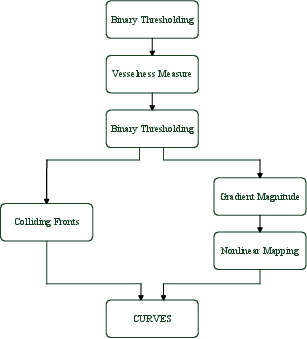
\includegraphics[height=3.2in,width=3.2in]{Figures/chap04/DataFlow.png}
\caption{Collaboration diagram of the segmentation pipeline.}
\label{fig:DataFlow}
\end{figure}

\subsection{Tubular Objects Enhancement}

The tubular enhancement is a sort of multi-scale line filtering, whose scheme can be summarized as the ``tube-like" objects in the image are highlighted whilst the rest are attenuated. %
To achieve this, the three dimensional multi-scale algorithm proposed by Sato \textit{et al.} \cite{Sato1998} is introduced.

To shape the filter response to certain width of lines and suppress the noisy effects, the pixels need to convolving with the second order derivatives of a Gaussian kernel.
This computation is an equivalent to the calculation of the Hessian matrix $\mathcal{H}$ of the three-dimensional image $I(\cdot)$:
\begin{gather}
\label{eqn:Hessian}
\mathcal{H} = \nabla^2 I =
\begin{bmatrix}
I_{xx} & I_{xy} & I_{xz} \\ I_{yx} & I_{yy} & I_{yz} \\ I_{zx} & I_{zy} & I_{zz}
\end{bmatrix},
\end{gather}
where $I_{xx} = \frac{\partial^2 I}{\partial^2 x}$, $I_{xy} = \frac{\partial^2 I}{\partial x \partial y}$, to name a few.
And all these partial second order derivatives are the convolutions with the second order derivatives of a Gaussian kernel $G(x; \sigma)$ with the standard deviation $\sigma$:
\begin{equation}
\label{GaussianConvolution}
I_{xx} = I \ast \frac{\partial^2 G}{\partial^2 x}.
\end{equation}
The eigenvalues of (\ref{eqn:Hessian}) are $\lambda_1$, $\lambda_2$, and $\lambda_3$ with their values in descending order.
Their associated eigenvectors are $e_1$, $e_2$, and $e_3$, respectively.

When $\lambda_1 \approx 0$ and $\lambda_2 \approx \lambda_3 \ll 0$, the line measure can be written as
\begin{equation}
\label{eqn:LineMeasure}
\lambda_{123} =
\begin{cases}
\left| \lambda_3 \right| \left( \frac{\lambda_2}{\lambda_3} \right)^{\gamma_{23}} \left( 1 + \frac{\lambda_1}{\left| \lambda_2 \right|} \right)^{\gamma_{12}}, & \lambda_1 \le 0 \\
\left| \lambda_3 \right| \left( \frac{\lambda_2}{\lambda_3} \right)^{\gamma_{23}} \left( 1 - \alpha \frac{\lambda_1}{\left| \lambda_2 \right|} \right)^{\gamma_{12}}, & \frac{\left| \lambda_2 \right|}{\alpha} > \lambda_1 > 0 \\
0, & \text{otherwise}.
\end{cases}
\end{equation}
In (\ref{eqn:LineMeasure}), the additional parameters $\gamma_{12}$, $\gamma_{23}$, and $\alpha$ are all positive constant, where $\gamma_{12} \in [0, \infty)$ is used to discriminate between the branching structures and the noises as well as pseudo-branches, $\gamma_{23} \in [0, \infty)$ regulates the sharpness, and $\alpha \in (0, 1.0]$ maintains the asymmetrical characteristics of the last terms of the function for all possible $\lambda_1$.

Additionally, different choices of the eigenvalues can equip the line filter with the abilities in detecting different shapes of the objects as shown in Table. \ref{tbl:Eigenvalues}. %

\subsection{Preprocessing for Level Set Evolution}

\subsubsection{Speed Images Calculation}

Level set algorithms evolves the contours in the gradient field with ``sharp" variations in intensity values from the inner or outer area to the boundaries.
The aim of the speed images is to provide this gradient field in the form of nicely shaped gradient images.
In the gradient images, the magnitude of the gradient at each pixel is calculated.
Next the gradient images $I_{\nabla}$ are transformed into the speed images $I_{\sigma}$ by applying the nonlinear relation:
\begin{equation}
\label{eqn:Sigmoid}
I_{\sigma} = (I_{max} - I_{min}) \cdot \frac{1}{1 + \exp\left(-\frac{I_{\nabla} - n}{m}\right)} + I_{min},
\end{equation}
where $I_{max}$ and $I_{min}$ are the two extreme values of the output intensity values, $m$ is a constant that controls the window width of the input intensity, and $n$ is a constant that defines the center of the window.
\begin{table}
\renewcommand{\arraystretch}{1.3}
\caption{Eigenvalue sets for detecting different shapes}
\label{tbl:Eigenvalues}
\centering
\begin{tabular}{l||c}
\hline
\bfseries Shape & \bfseries Eigenvalues \\
\hline\hline
Bright tubes   & $\lambda_1 \approx 0, \lambda_2 \approx \lambda_3 \ll 0$ \\
Dark tubes     & $\lambda_1 \approx 0, \lambda_2 \approx \lambda_3 \gg 0$ \\
Bright plates  & $\lambda_1 \approx \lambda_2 \approx 0, \lambda_3 \ll 0$ \\
Dark plates    & $\lambda_1 \approx \lambda_2 \approx 0, \lambda_3 \gg 0$ \\
Bright spheres & $\lambda_1 \approx \lambda_2 \approx \lambda_3 \ll 0$ \\
Dark spheres   & $\lambda_1 \approx \lambda_2 \approx \lambda_3 \gg 0$ \\
\hline
\end{tabular}
\end{table}

\subsubsection{Initial Contours Evolution Using Colliding Fronts}

The aim of the colliding fronts module is to evolve the contours for the CURVES system from the user-defined seeding points.
The colliding fronts method is implemented based on the principles of the fast marching algorithm \cite{Sethian1999}.
However, this method requires two seeds for each round of evolution such that the area between the seeds can be extracted.
The output of this module is the dot production of the gradient field of arrival times of the two wavefronts.
The level set initialization for the prolonged objects greatly benefit from this feature of the method.
On the other hand, the method also shortens the computation time.

\subsection{CURVES Evolution Model}

The CURVES method \cite{Lorigo2001} is chosen as the functioning segmentation method because of the complex nature of the coronary arteries.
It is highly effective in the segmentation of the complicated curvilinear structures in the volumetric medical images.
In addition, the criterion of CURVES method also takes the local smoothness of the boundaries to be detected (i.e., the inner wall of the coronary arteries) into account.

This method is a modification of the geodesic active contours method developed in Caselles \textit{et al.} \cite{Caselles1997}.
As the extensive research of the geodesic active contours, CURVES is a level set algorithm that models the tiny vessels as spatial curves with arbitrarily complicated topology \cite{Lorigo2001}. %
CURVES evolves the level sets to the boundaries of the targets based on the criterion of the minimization of the following energy functional
\begin{equation}
\label{eqn:CURVES}
\oint_0^1 g\left( \left| \nabla I \left( \mathcal{C} \left(  s \right) \right) \right| \right) \left| \mathcal{C}'\left( s \right) \right| ds,
\end{equation}
where $\mathcal{C}\left( s \right): [0,1] \rightarrow \mathrm{R}^3$ is a one-dimension curve, $I\left( \cdot \right): [0, a] \times [0, b] \times [0, c] \rightarrow [0, \infty)$ is an image on which the curve evolution takes place, and $g\left( \cdot \right): [0, \infty) \rightarrow \mathrm{R}^+$ is a monotonically decreasing function. %

The minimization of this functional can be achieved by searching for the gradient descent direction of the functional itself, which means the Euler-Lagrange equations associated with (\ref{eqn:CURVES}) needs to be computed. %
Thus the geodesic flow equation that controls the contour evolution in this process of minimization can be obtained as follows
\begin{equation}
\label{eqn:Evolution}
\frac{\partial \mathcal{C}}{\partial t} = k \mathcal{N} - \frac{g'}{g} \varPi \left( \mathcal{H} \frac{\nabla I}{ \left| \nabla I \right| } \right),
\end{equation}
where $\mathcal{H}$ is the Hessian matrix of the image $I$, $k$ is the Euclidean curvature, $\mathcal{N}$ is the unit normal vector, $\varPi(\cdot)$ is the projection operator projects the argument onto the normal space. %
The update equation can be obtained as
\begin{equation}
\label{eqn:Update}
\frac{\partial v}{\partial t} = \mathcal{F} \left( \nabla v(x, t), \nabla^2 v(x, t) \right) + \frac{g'}{g} \nabla v(x, t) \mathcal{H} \frac{\nabla I}{ \left| \nabla I \right| },
\end{equation}
where $v(\cdot): \mathrm{R}^3 \rightarrow [0, \infty)$ is the embedding function of the curve $\mathcal{C}$, $\mathcal{F} \left( \nabla v(x, t), \nabla^2 v(x, t) \right)$ is the smaller eigenvalue of the matrix $P_{\nabla v} \nabla^2 v P_{\nabla v}$. %
The matrix $P_q$ is defined as a projector which projects some vector onto the normal plane of vector $q \in \mathrm{R}^3$:
\begin{equation}
\label{eqn:ProjectionOperator}
P_q = I_0 - \frac{qq^T}{\left| q \right|^2},
\end{equation}
where $I_0$ denotes the identity matrix.

By incorporating the speed images $I_{\sigma}$ to the evolution equation (\ref{eqn:Evolution}), the evolution in our case can be obtained as
\begin{equation}
\label{eqn:Application}
\frac{\partial \mathcal{C}}{\partial t} = k \mathcal{N} - \frac{g'(I_{\sigma})}{g(I_{\sigma})} \varPi \left( \mathcal{H} \frac{\nabla I_{\sigma}}{ \left| \nabla I_{\sigma} \right| } \right).%
\end{equation}

\subsection{Surface Rendering}

The surface information is extracted for the visualization by the marching cubes method \cite{Lorensen1987MC}.
Cubes are created based on the input information and are organized into an array structure.
Each cube consists of eight pixels (each four pixels are from a slice).
The index of each cube is labeled by comparing the intensity values of every pixel to the isovalue of the surfaces.
Next the patterns of the intersection between objects and cubes are initially determined based on the triangulated cases.
Then the precise intersection are computed using linear interpolation with the intensity values at each vertex.
The unit normals to the surface are calculated via central differences for the vertices of the cubes.
Finally the generated triangles are ready for the surface rendering.

\section{Experiments and Results}

\subsection{Medical Data and Experimental Setup}

The original chest CTA series was acquired by a 128-slice Siemens SOMATOM Definition Flash CT.
The slice thickness was $0.6 \text{mm}$ and the in-slice resolution was $0.4 \times 0.4 \text{mm}^2$.
Since the work was all on the coronary arteries, the volume contained the whole heart (i.e., ROI, which is the abbreviation of \textit{region of interest}) was cropped from the original data as shown in Fig. \ref{fig:Original}. %

Numbers of experiments were conducted with different sets of parameters to segment the coronary arteries from CTA for the testament of the approach in this paper.
In our case, the original CTA series in DICOM format had been converted to the form of XML first; and the data type of pixels are converted for the incoming computation.
Next the converted data was enhanced by the module which was implemented based on the algorithm developed in \cite{Sato1998}.
Then the tubular enhanced data was send to the following modules to perform calculations of speed image production and input level sets generation.
The two set of the resulting data from the two computation pipelines were transferred to the CURVES module in order to generate the final fronts evolution results.
Finally, the marching cubes method was employed to extract the iso-surface corresponding to the wall of the coronary arteries.
All the experiments were performed on a machine with Intel's 2.83GHz Core 2 Quad CPU and 4GB RAM.

\subsection{Tubular Enhancement and Its Postprocessing}

Before the tubular enhancement started, a global binary thresholding was performed in order to provide the enhancing filter with the focus on the tiny bright tubular objects.
To achieve this, the thresholder was called to trim the irrelevant contents in the images, e.g., dark lung regions with negative intensity values, bright bone regions with large positive intensity values, etc. %
As shown in Fig. \ref{fig:Binary1}, the intensity values of the regions within the interval between the lower threshold and the upper threshold were uniformly assigned a unique intensity value, i.e., $255$ in our case; the intensity values of the rest regions were uniformly assign a zero intensity value. %

Referring to the shape prior guidelines listed in Table. \ref{tbl:Eigenvalues}, the tubular enhancement filter was fed the parameters to detect the bright tubular objects, i.e., coronary arteries. %
Among these parameters, $\sigma$ controls the diameter of cross-section of the tubular objects to be enhanced, $\gamma_{12}$ is the measure of the tube similarity, and $\gamma_{23}$ is used for the recovery of vessel regions with inhomogeneous contrast or intensity loss. %
As shown in Fig. \ref{fig:Vesselness}, the tiny vessels including the coronary arteries and the vessels in lung areas were enhanced with a small $\sigma$ whilst the tubular structures with cross-section diameters larger than this value were not enhanced. %

The intensity values of the enhanced tubular objects were relatively low and scattered in a wide range.
This is a mass for the selection of the intensity value in the following processing steps.
To deal with it and facilitate this situation, some intensity transformation step was needed.
The nonlinear intensity mapping filter and the binary threshold filter were the candidates.

Equation (\ref{eqn:Sigmoid}) showed that the nonlinear intensity mapping transformed the input image into the image with partial enhancement and partial attenuation.
With the well chosen parameters, the intensity values corresponding to the targeting objects in this case were enlarged and the rest part of the images in lower intensities were all depressed as near zero intensity areas. %
Because of the mapping characteristics of the sigmoid functions, the intensity values of the bright tubular structures were not uniformly distributed and stayed at the relatively low levels (see Fig. \ref{fig:Sigmoid}). %
In another test, the binary threshold filter extracted the pixels with the intensities in the specified range and assigned them with a unique large intensity value as discussed above (see Fig. \ref{fig:Binary2}). %
Comparing the result of the two candidates, the binary threshold filter was selected to improve the results of the precedent tubular enhancement filter (see Fig. \ref{fig:DataFlow}). %
\begin{figure}[t]
\centering
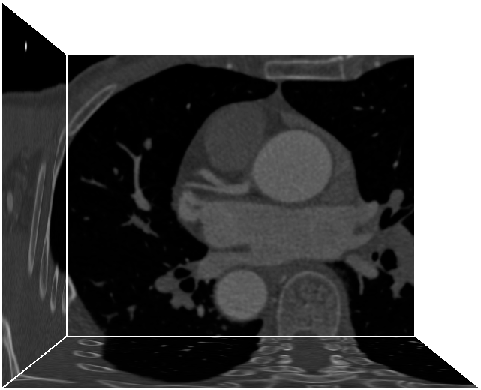
\includegraphics[width=2.8in]{Figures/chap04/original.png}
\caption{Original ROI-extracted volumetric data}
\label{fig:Original}
\end{figure}
\begin{figure}[t]
\centering
\subfloat[]{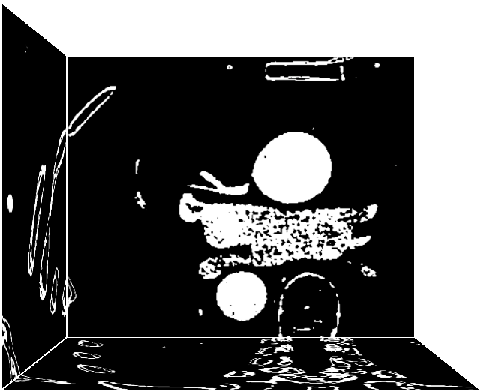
\includegraphics[width=2.8in]{Figures/chap04/binary1.png}%
\label{fig:Binary1}}
\hfil
\subfloat[]{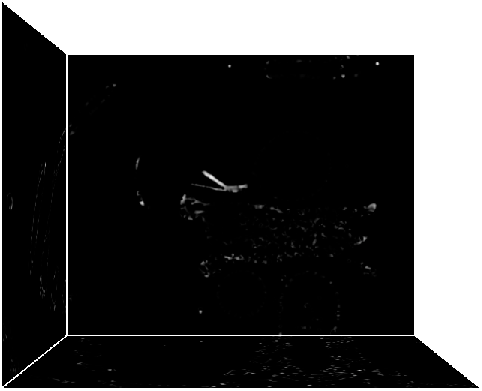
\includegraphics[width=2.8in]{Figures/chap04/hessian.png}%
\label{fig:Vesselness}}
\caption{Preprocessing results of the original CTA images based on the ``vesselness" measure: (a) binary thresholding ($\text{lower threshold} = 300$, $\text{upper threshold} = 600$) (b) tubular enhancement ($\sigma = 0.9$, $\gamma_{12} = 0.1$, $\gamma_{23} = 2.0$).}%
\label{fig:Preprocessing}
\end{figure}

\subsection{Feature Images Computation}

To generate the feature images for the CURVES system, two steps were performed:
(1) calculating the gradient magnitude at each pixel; and
(2) converting the gradient images into the speed images.
%\begin{enumerate}
%\item calculating the gradient magnitude at each pixel;
%\item converting the gradient images into the speed images.
%\end{enumerate}
The gradient magnitude module computed the magnitude of the gradient pixel-wisely for the image by performing the convolution with the first order derivatives of a Gaussian kernel.
The wall of the tiny vessels were extracted before the nonlinear intensity mapping was employed to generate the edge potential maps.
The extreme values of the pixel intensities in the gradient magnitude images directly effected the selection of the parameters in (\ref{eqn:Sigmoid}).
To reverse the lightness of the objects (in low intensities in the gradient magnitude images) and its edges (in high intensities in the gradient magnitude images), $n$ was chosen to be the center of the intensity window containing the vessels, and $m$ a negative value with $|m|$ as the width of the window. %
The minus sign of $m$ means the reverse operation on the pixels.
The neighborhood of the boundaries of the objects were in almost zero intensity, which made the evolution driven by (\ref{eqn:Application}) faster in the ``plateau" (with uniformly high intensities), whilst much slower (in a speed of about zero) in the ``ridges" (with rapid decreasing intensities). %

\subsection{Wave Fronts Propagation}

The initial level sets were evolved by the colliding fronts module.
Two seeds were located interior of the regions corresponding to the coronary arteries and the interfaces surrounding each seeds evolved towards each other.
The dot production of the gradients of arrival times of the two wavefronts were computed.
\begin{figure}[t]
\centering
\subfloat[]{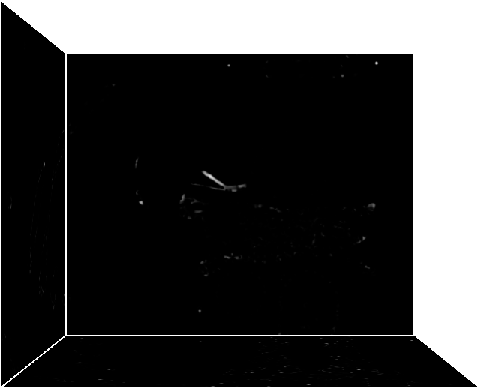
\includegraphics[width=2.8in]{Figures/chap04/sigmoid.png}%
\label{fig:Sigmoid}}
\hfil
\subfloat[]{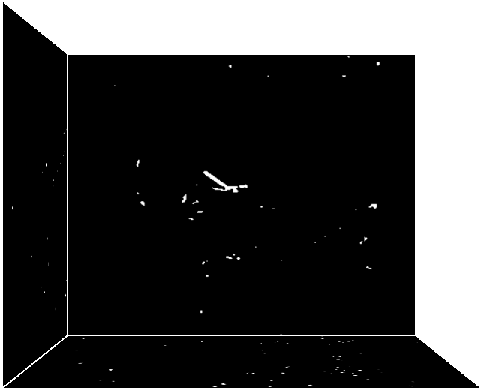
\includegraphics[width=2.8in]{Figures/chap04/binary2.png}%
\label{fig:Binary2}}
\caption{Comparison of the two different intensity conditioning approaches: (a) nonlinear intensity mapping ($m = 80$, $n = 120$); (b) binary thresholding ($\text{lower threshold} = 40$, $\text{upper threshold} = 200$).}%
\label{fig:IntensityConditioning}
\end{figure}
\begin{figure}[t]
\centering
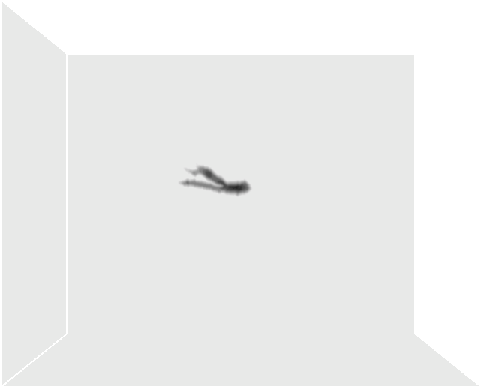
\includegraphics[width=2.8in]{Figures/chap04/curves.png}
\caption{CURVES evolution based on the initial contours generated by the colliding fronts method and the edge feature maps calculated by the nonlinear intensity mapping function.}%
\label{fig:CURVES}
\end{figure}
\begin{figure*}[t]
\centering
\subfloat[]{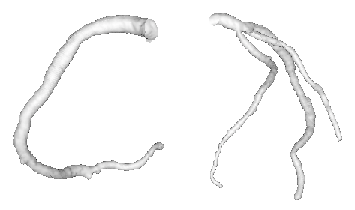
\includegraphics[width=2.8in]{Figures/chap04/model_conventional.png}%
\label{fig:VisualizationModelCURVES}}
\hfil
\subfloat[]{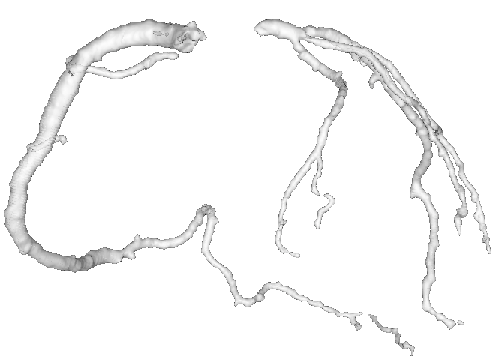
\includegraphics[width=2.4in]{Figures/chap04/model_enhanced.png}%
\label{fig:VisualizationModelTECURVES}}
\caption{Models of the coronary arteries: (a) conventional CURVES evolution; (b) tubular-enhanced CURVES evolution.}%
\label{fig:VisualizationModel}
\end{figure*}

The CURVES system started working when all the preceding calculation completed.
The module took the speed images as its evolution maps and the initial contours as its initial states and regulates the evolution according to (\ref{eqn:Application}).
The evolution terminated when the contours evolved against the wall of the coronary arteries in the specified steps of iterations.
And the resulting evolution extracted the coronary arteries as shown in Fig. \ref{fig:CURVES}.
Next a binary thresholding step was provoked to label the inner area of the coronary arteries with high intensity value whilst the outer area with zero intensity value.

\subsection{Visualization of Segmentation Results}

By manually picked the isovalue corresponding to the wall of the coronary arteries, the resulting volume were processed using the marching cubes method \cite{Lorensen1987MC}.
The visualization models of the coronary arteries respectively based on the CURVES regions without and with tubular enhancement demonstrated their capabilities of displaying the complicated geometrical details (see Fig. \ref{fig:VisualizationModelCURVES} and \ref{fig:VisualizationModelTECURVES}). %

\section{Conclusions and Future Work}
%The conclusion goes here.

The three dimensional visualization of the blood vessels plays an important role in the construction of the virtual scenario for the robotic surgical simulator.
Further, the visualization of the coronary arteries is the most critical and difficult work.
Because of the complex spatial topologies, details can be easily lost in the process of segmentation.
In this paper, a vasculature segmentation method based on tubular-enhanced CURVES has been developed.
Then the process of the experiment was presented and the results were demonstrated.
The experimental results showed that the proposed approach is capable of enhancing the tiny dark vessels and visualizing the geometric details of them.

The tubular feature of coronary arteries was enhanced and the speed images were generated.
Meanwhile, the initial contours for the CURVES method were computed by a modified version of fast marching method in another process.
The actual level sets evolution began after the above computation finished and the evolution took a specified number of iterations to detect the coronary arteries.
At the end of the segmentation, the resulting pixels were all conversed in their intensities.
Finally the data representing the surface of the arteries was extracted by the marching cubes method.

Our future plans are the further optimization of the blood vessel models for the simulation with virtual tools of the robotic surgical simulator.
The principle work will be the decimation of the quantity of the triangles consisting the blood vessels and the improvements of the visualization effects of the virtual scenario. 
%# -*- coding:utf-8 -*-
\chapter{血管模型中心线的提取}
\label{chap7}

\section{Introduction}
% no \PARstart
Cardiovascular diseases are among the most fatal illnesses worldwide \cite{WHO2013}.
The diseases occur when the stenosis or even blockages formed due to the build up of fatty substances on the inner wall of the blood vessels.
Percutaneous coronary intervention (PCI) is the gold standard in fighting the lethal diseases.
Due to its minimally-invasive nature, this procedure only causes small incision and much less trauma to the patients.
In addition, the hospitalization after the procedure is in turn dramatically shortened.
However, due to the very nature of minimally-invasiveness of PCI and the complex anatomic structure of the blood vessels, the learners need thorough and strict training before performing the procedure in action. %
What's worse, the practitioners in catheterization labs have to expose themselves under the ionizing radiation from the fluoroscope while examining the morphologies of the patients' vasculature. %

The surgical robotic systems for intravascular procedures have greatly changed this situation.
With the assistance of the robotic systems, cardiology practitioners need not to be worried about the radioactive exposure and the relative risks any more.
Like their ancestors (i.e., the traditional PCI procedure), the skills of manipulating the robotic system to do the surgery are also not easy for the junior residences and still require strict and sufficient training before applying the procedure on the real patients. %

The traditional ways of training PCI procedure are deeply rooted in the physical fashion, i.e., employing biological models (e.g. human cadavers and living animals) or non-biological models (e.g. phantoms). %
The former are disposable and ethic-disputed; let alone the tremendous expenditure on the preservation and feeding, and the distinction in anatomy between human and animal volunteer. %
The latter are stiff and lack of sufficient anatomic details, even though they can be used repeatedly.
Indeed, it is infeasible to conduct the training on the expensive robotic systems whilst ignoring the real needs in the catheterization labs.
To streamline the training and the practice of robotic PCI procedure, a well-designed computing simulation system is required.

The aim of our effort is to provide a training tool of convenience and effectiveness for the minimally-invasive intravascular robotic system \cite{Ji2011EMBC}.
In constructing this training vehicle, the anatomic structures in computing environment especially the vascular system are definitely one of the most substantial components.
The centerlines is an effective way of describing the shape of the model \cite{Ogniewicz1995}, which will provide accurate shape description for the path planning in interactive simulation.
In this paper, we developed an automatic approach based on the Voronoi diagram \cite{Antiga2003} to extract the centerlines of the vasculature.
The input of the proposed approach is the patient-specific image-based surface model of the vasculature, which is reconstructed by applying our previous work \cite{Yang2014ICRA}. %
Before computing the Voronoi diagram of the tubular surface model, several preprocessing should be performed.
First, the connectivity of the polygons that consisting the surface is validated thoroughly to include the largest connected polygons that is effective in representing the surface. %
Second, the bumpy and crusty surfaces are smoothed in order to reduce the effects on the computation of centerlines.
Third, the surfaces are subdivided to gain a more precise geometric feature.
Finally, the centerlines of the vessel model by solving the Eikonal equation in the fast marching flavor.
The capability of our approach in automatically extracting the centerlines of the vessel model is proved by the experimental results.

The rest of this paper is organized as follows.
Section II introduces the related work of the centerline extraction methods for three dimensional objects.
Section III outlines the work flow and describes the techniques used in this work.
Section IV describes the experiments, ending with a brief discussion.
The final section concludes the whole work.

\section{Related Work}

Many researches have been done since the earliest work on extracting the centerline was proposed by Blum \cite{Blum1967}.
According to reference \cite{Ogniewicz1995}, most of these methods fall into four categories: (1) topological thinning; (2) distance transformation; (3) ``prairie fire" approach; (4) Voronoi Diagram methods. %

Topological thinning methods \cite{Ma2002,Sadleir2002} implement the centerline extraction by iteratively remove most of the ``simple points" except the ones that are the end-points of the generated centerline models. %
By ``simple points", it means that the boundary points consisting the object such that their removals do not destroy the topology of the object.

Distance transformation methods \cite{Niblack1992} find the centerline by searching the local maximum among the minimal distances between the points interior of the shape and the boundary. %
However, they do not ensure the resulting centerlines are connected with each other.

``Prairie fire" methods \cite{Blum1967,Leymarie1992} compute the centerline by determining the intersection of the propagating interfaces with their sources located on the boundary of the shape. %

Voronoi diagram method \cite{Sherbrooke1996,Antiga2003} treats the centerline to be generated as a subset of the Voronoi diagram.
These methods are sensitive to the noises and the regularization of the boundary of the shape.

There are numbers of other methods that are not belong to any category listed above.
Ferchichi and Wang in \cite{Ferchichi2006} reported a clustering-based algorithm for centerline extraction both for 2D and 3D objects.
The algorithm was designed based on the idea of computing the maximal disks/balls determining the centerlines, which is achieved by executing the K-means algorithm iteratively on the object-points and their distance transforms. %
Egger \textit{et al.} \cite{Egger2007} reported a centerline extraction algorithm for the blood vessels using Dijkstra's shortest path algorithm, which was designed for the catheter simulation. %

\section{Methodologies}

This section discusses the design of the processing pipeline and details the principles of the consisting modules.
Before the actual centerline extraction begins, several processing aims to removing noises and smoothing the irregular surfaces need to be run to guarantee the quality of the input surface.
The image-based surface model of the blood vessels needs series of postprocessing steps depicted in Fig. \ref{fig:DataFlow} to meet the requirements of the centerline computing module. %
Among these processing steps, the first one is the validation of the connectivity of the consisting polygons.
During this process, the largest possible connected regions of the surface model are extracted.
Next, the surface smoothing step is needed to depress the ``crusts" and ``stairs" in the surface.
Then the normal vectors (i.e., normals) are computed to mark the ``inside" and the ``outside" of the surface model.
After that, the consisting polygons need to be subdivided under a specified criterion to facilitate the computation of the centerline extraction at the cost of longer computation time. %

%\subsection{Processing on Image-Based Surface Model}

\subsection{Connectivity Validation and Largest Region Extraction}

In this paper, the vasculature surface model is generated from the original medical volumetric data set by applying the approaches reported in our previous work \cite{Yang2014ICRA}. %
In order to find the largest region spanning the surface of the vasculature, the connectivity among the vertices in the image-based surface model needs to be thoroughly validated at the beginning of the processing. %
The inner working is to extract consisting polygons that share common vertices and meet some requirements.
In the present paper we implement the algorithm to extract the largest connected region from the input surface.
\begin{figure}[t]
\centering
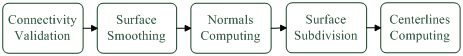
\includegraphics[width=3.2in]{Figures/DataFlow3.png}
\caption{Overview of the work flow.}
\label{fig:DataFlow}
\end{figure}

\subsection{Surface Smoothing and Normals Computing}

There are plenty of methods used for the surfaces smoothing in visualization.
To overcome the ``facets" by-produced during this approximation, an optimal surface smoothing algorithm treating this problem as low-pass filtering by extending Fourier analysis is adopted \cite{Taubin1996}. %
The adopted method is built upon the formulation of the \emph{discrete graph signals}, which means the functions based on directed graph.
The directed graph $G$ represents the polyhedral surfaces in this problem, which is denoted as the set $\left\{ 1, \ldots, n \right\}$ of nodes with a set of neighborhoods $\left\{ i^{\ast}: i = 1, \ldots, n \right\}$ of node $i$. %
A discrete graph signal can be represented as a vector $x = \left[ x_1, \ldots, x_n \right]^T$, where each component of the vector corresponds one node of the graph.
A polyhedral surface $S = \{ V, F \}$ of $n$ vertices can be treated as a directed graph, where the vertices $V$ corresponds the set of nodes $n$ and the faces $F$ the polygons formed by connected nodes. %

The discrete surface signal, the discrete graph signal defined on the associated graph, can be visualized as a piece-wise linear function defined on the surface.
The computation of the Discrete Fourier Transform (DFT) of the discrete surface signal defined on the surface is achieved by decomposing the surface signals as a linear combination of the eigenvectors of the Laplacian: %
\begin{equation}
\label{eqn:Laplacian}
\Delta x_i = \sum_{j \in i^{\ast}} w_{ij} \left( x_j - x_i \right),
\end{equation}
where $w_{ij}$ is the positive weight for each difference of $x_j - x_i$ and for a given vertex $i$, the sum of its weights are always one.
The matrix form of (\ref{eqn:Laplacian}) is
\begin{equation}
\label{eqn:LaplacianMatrix}
\Delta x = - K x,
\end{equation}
where $K = I - W$, with $I$ an identity matrix and $W$ the matrix of weights $w_{ij}$.

Choosing $0 \leq k_1 \leq \ldots \leq k_n \leq 2 $ as the eigenvalues of $K$, $r_1, \ldots, r_n$ the corresponding right eigenvectors, and $d_1, \ldots, d_n$ the associated dual basis of these eigenvectors, the above $K$ can be obtained as $K = \sum_{i} k_i r_i d_i^T$. %
%\begin{equation}
%\label{eqn:K}
%K = \sum_{i} k_i r_i d_i^T.
%\end{equation}
Thus there is a unique decomposition the discrete graph signal $x$, which can be obtained as a linear combination of the right eigenvectors $x = \sum_{i} \hat{x}_i r_i$, %$r_1, \ldots, r_n$
%\begin{equation}
%\label{eqn:x}
%x = \sum_{i} \hat{x}_i r_i,
%\end{equation}
where $\hat{x}_i = d_i^T x$ is the DFT of $x$.

According to signal processing theory, the filtering calculation on the signal $x$ is to change its frequency distribution at the reference of a transfer function $f$:
\begin{equation}
\bar{x} = \sum_{i} f(k_i) \hat{x}_i r_i = \left( \sum_{i} f(k_i) r_i d_i^T \right) x.
\end{equation}
The \emph{low-pass filtering} mechanism can be implemented by adjusting the weights in the following polynomial approximation
\begin{equation}
\label{eqn:Approximation}
f_{N}(k) = w_0 \frac{\theta}{\pi} T_0 (1 - k / 2) + w_n \sum_{n} \frac{2 \sin (n \theta)}{n \pi} T_n(1 - k / 2),
\end{equation}
where $\theta$ is the unique solution of $k = 2 (1 - \cos \theta)$ on $[0, \pi / 2]$, and $T$ the Chebyshev polynomial.
Here in this paper, the weights in (\ref{eqn:Approximation}) is adjusted to form a Hamming window, among sorts of them, which is demonstrated as follows:
\begin{equation}
\label{eqn:HammingWindow}
w_n = 0.54 + 0.46 \cos (n \pi / (N + 1) ).
\end{equation}

The normal vectors to the surfaces are computed after the surfaces are smoothed.

\subsection{Surface Subdivision}

A modified butterfly scheme for surface subdivision is used in order to refine the smoothed surface model \cite{Zorin1996}.
This scheme is designed in the flavor of interpolating and has been proved to be useful in the circumstances of subdivision for the complex especially irregular surfaces.
The ultimate goal is to improve the visualization of the input surface model without affecting its original shape.
The scalar value associated with the new vertex of the 2-dimensional triangulation is generated by calculating weighted sum of neighboring vertices using the proposed interpolation scheme. %
These vertices located in the neighborhood form the subdivision stencil, which determines the features of the scheme.
By analyzing the stencil, the scheme can quickly identify the relationship between the new vertex and the topology of its neighborhood.
The two most important cases in the surface are the regular sites and the extraordinary sites.
Once the initial subdivision cycles completed, the largest number of the vertices possessing the valence other than six is not exceeding one.
The new scalar value for the midpoint on each edge of the triangulation is calculated by the subdivision scheme falls into the following cases:
(1) edge connects two regular vertices;
(2) edge connects an extraordinary vertex and a regular vertex;
(3) edge connects two extraordinary vertices; and
(4) boundary edges.
%\begin{itemize}
%\item edge connects two regular vertices;
%\item edge connects an extraordinary vertex and a regular vertex;
%\item edge connects two extraordinary vertices;
%\item boundary edges.
%\end{itemize}
Among the above cases, only the first one belongs to the regular case, whilst the rest belong to the extraordinary case.

\subsection{Centerlines Extraction}

Centerlines, or medial axis, can be generally defined as the loci of the centers of the maximal inscribed disks (in 2D space) or spheres (in 3D space) inside an object.
Conversely, the envelop of all maximal inscribed disks/spheres is the boundary/surface of the object that contains these disks/spheres \cite{Amenta2001}.
Our approach employed the method demonstrated in \cite{Antiga2003}, which treats the centerlines as the minimal action paths on the Voronoi diagrams inside the model surface.
The Voronoi diagrams are the discrete approximation of the medial axis of the shape in two or three dimensional space.
The minimization of the line integral of the action path, which links two vertices in the Voronoi diagram, generates the center points that locally maximize their minimal distances to the boundary of the surface.
To do this, the method firstly computes the following Eikonal equation from a given starting point located on the Voronoi diagram
\begin{equation}
\label{eqn:Voronoi}
\left| \nabla T \right| = \frac{1}{R(u)},
\end{equation}
where $T$ marks the time of arrival, $R$ the radius of the maximal inscribed sphere at the time $T$, and $u$ the parametric space of the Voronoi diagram.
Then the centerline is obtained by calculating the following equation upon the previously demonstrated computation terminated:
\begin{equation}
\label{eqn:Centerlines}
\frac{dc}{ds} = - \nabla T,
\end{equation}
where $c$ denotes the centerlines, and $s$ the parametric space of $c$.
As a matter of fact, computation illustrated by (\ref{eqn:Centerlines}) is equivalent to finding the resulting centerline by applying the steepest descent method at each point on the Voronoi diagram.

\section{Experiments and Discussions}

\subsection{Data and Experimental Setup}

The vasculature surface models were generated by applying the approaches proposed in \cite{Yang2014ICRA} from the original CTA images acquired from some real patient.

In our experiments, the programs written in C++ ran on a desktop with Intel's 2.83GHz Core 2 Quad CPU and 4GB RAM.
%For the simplicity of description, part of the abdominal aorta is chopped off to serve as the sample data in our experiments described here (see Fig. \ref{fig:VOI}). %
Part of the abdominal aorta was chopped off to serve as the sample data in our experiments described here (see Fig. \ref{fig:VOI}). %
The approach can be applied straightly to the surface model of the whole abdominal aorta (see Fig. \ref{fig:OverlayGlobal}). %and Fig. \ref{fig:VisualizationModel}).
\begin{figure}[t]
\centering
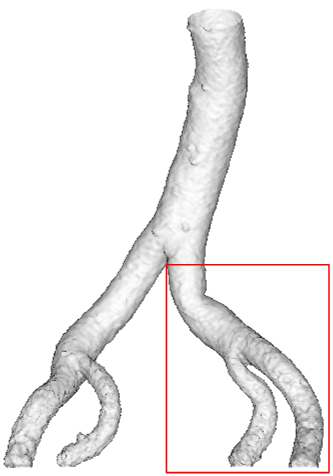
\includegraphics[height=2.4in]{Figures/VOI.png}
\caption{The original model surface (consists of $205,590$ polygons) and the VOI-extracted local part (in red square).}
\label{fig:VOI}
\end{figure}

%\subsection{Preprocessing for Centerline Extraction}

\subsection{Validating Connectivity of Image-Based Surface Model}

Before actually extracting the centerlines, the image-based surface model of the vasculature needs to be properly conditioned such that the computation can be operated successfully. %
The initial pass is the validation of the connectivity among the adjacent polygonal surfaces that consists of the whole visualization model.
The aim of this step is to find and connect the largest connected region in the given surface model (see Fig. \ref{fig:ConnectivityLocal}).
Table \ref{tbl:Connectivity} shows that the quantities of the consisting polygonal surfaces were not changed in local cases, whilst were decreased in global cases.
The former implies that the given (local) model was the largest connected region in the surface model before the validation.
The latter indicates that the largest connected region of the given model surface was fully extracted through the validation.
\begin{figure}[t]
\centering
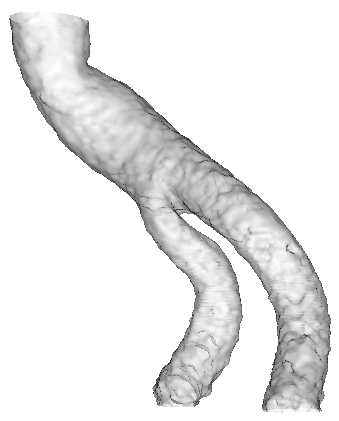
\includegraphics[width=1.5in]{Figures/connectivity_local.png}
\caption{Results of connectivity validation of model surface in local details (quantity of consisting polygons: $70,625$).}
\label{fig:ConnectivityLocal}
\end{figure}

\begin{table}[t]
\renewcommand{\arraystretch}{1.3}
\caption{Quantities of polygons before and after connectivity validation}
\label{tbl:Connectivity}
\centering
\begin{tabular}
{@{}llr@{}}
%{@{}llrr@{}}
\toprule
%\hline
%~      & ~                       & \multicolumn{2}{c}{Quantities} \\
%\cmidrule(4){3-4}
%~      & ~                       & Vertices & Polygons            \\
~      &                         & Quantities of polygons \\
%\midrule
\hline\hline
%Local  & Before validation       & N/A      & 70,625  \\
%~      & After validation        & N/A      & 70,625  \\
Local  & Before validation       & $70,625$  \\
~      & After validation        & $70,625$  \\
\hline\hline
%Global & Before validation       & N/A      & 205,590 \\
%~      & After validation        & N/A      & 205,452 \\
Global & Before validation       & $205,590$ \\
~      & After validation        & $205,452$ \\
\bottomrule
%\hline
\end{tabular}
\end{table}
\begin{figure}[t]
\centering
\subfloat{\includegraphics[width=1.5in]{Figures/smooth_30_1_local.png}%
\label{fig:Smooth30-1Local}}
\hfil
\subfloat{\includegraphics[width=1.45in]{Figures/smooth_30_01_local.png}%
\label{fig:Smooth30-01Local}}
\hfil
\subfloat{\includegraphics[width=1.5in]{Figures/smooth_100_1_local.png}%
\label{fig:Smooth100-1Local}}
\hfil
\subfloat{\includegraphics[width=1.45in]{Figures/smooth_100_01_local.png}%
\label{fig:Smooth100-01Local}}
\caption{Smoothing effects by applying different parameters: (a) $\text{pass band} = 0.1$, $\text{iterations} = 30$; (b) $\text{pass band} = 0.01$, $\text{iterations} = 30$; (c) $\text{pass band} = 0.1$, $\text{iterations} = 100$; (d) $\text{pass band} = 0.01$, $\text{iterations} = 100$.}%
\label{fig:SmoothLocal}
\end{figure}

%\begin{table}
%\renewcommand{\arraystretch}{1.3}
%\caption{Comparison of quantities of polygonal surfaces - Part I}
%\label{tbl:Eigenvalues}
%\centering
%\begin{tabular}{l||r}
%\hline
%\bfseries Connectivity validation & \bfseries Quantities \\
%\hline\hline
%Before                            & 757,538 \\
%After                             & 757,400 \\
%\hline
%\end{tabular}
%\end{table}

\subsection{Smoothing Connected Surface Model}

The centerline extracting method adopted in this work is sensitive to the noises on the input surface.
Due to the poor quality in some level of details of the original images, segmentation may introduce unnecessary uneven surfaces.
These artifacts in the surfaces can cause difficulties in the delivering of the virtual guidewires towards the hesion along the lumen of the model vessels.
To depress the noisy surface of the model, a surface smoothing module implemented based on low-pass filtering is applied.
There are two parameters associated with the smoothing module.
One of them specifies the number of iterations, which is equivalent to the degree of the polynomial approximating the windowed sinc function defined by (\ref{eqn:Approximation}).
The other determines the pass band of this low-pass filtering module.
Different sets of parameters were fed to the smoothing module in order to find the best results for the following processing (see Fig. \ref{fig:SmoothLocal}).
Observing these results, the parameters ($\text{pass band} = 0.01$, $\text{iterations} = 100$) used to generating the resulting surface in Fig. \ref{fig:Smooth100-01Local} demonstrated better effects than the rest.
%\begin{figure}[t]
%\centering
%\subfloat[]{\includegraphics[width=1.5in]{../Figures/smooth_30_1_local.eps}%
%\label{fig:Smooth30-1Local}}
%\hfil
%\subfloat[]{\includegraphics[width=1.45in]{../Figures/smooth_30_01_local.eps}%
%\label{fig:Smooth30-01Local}}
%\hfil
%\subfloat[]{\includegraphics[width=1.5in]{../Figures/smooth_100_1_local.eps}%
%\label{fig:Smooth100-1Local}}
%\hfil
%\subfloat[]{\includegraphics[width=1.45in]{../Figures/smooth_100_01_local.eps}%
%\label{fig:Smooth100-01Local}}
%\caption{Smoothing effects by applying different parameters: (a) $\text{pass band} = 0.1$, $\text{iterations} = 30$; (b) $\text{pass band} = 0.01$, $\text{iterations} = 30$; (c) $\text{pass band} = 0.1$, $\text{iterations} = 100$; (d) $\text{pass band} = 0.01$, $\text{iterations} = 100$.}%
%\label{fig:SmoothLocal}
%\end{figure}

\subsection{Subdivision Using Improved Butterfly Scheme}

To further attenuate the effects of noisy surfaces on extraction of centerlines and increase the precision of the centerlines extraction, the number of the polygons consisting the model surface has to be increased.
In order to achieve this, the smoothed surface need to be subdivided without introducing more perturbation.
Figure \ref{fig:SubdivisionLocal} illustrates that the subdivision computation based on the improved butterfly scheme.
At the same time, the quantities of the consisting polygonal surfaces increased substantially after the subdivision complete (see Table \ref{tbl:Subdivision}).
Comparing the quantities of the polygons before and after the subdivision in both cases, the quantities of the resulting polygons are about four times greater than the quantities of the input polygons due to the subdivision scheme employed in this work.
\begin{figure}[t]
\centering
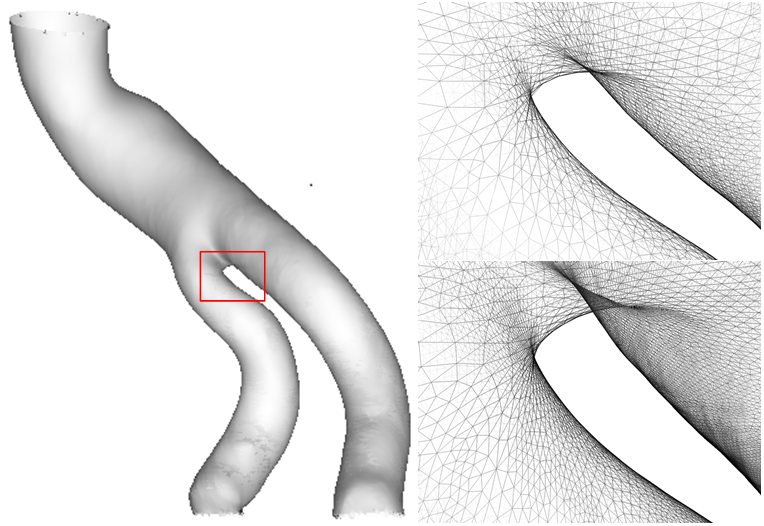
\includegraphics[width=3.0in]{Figures/subdivision.png}
\caption{Subdivision of smoothed surface by using improved butterfly scheme. \emph{Left}: subdivision in local details. \emph{Top right}: polyhedral surface before subdivision. \emph{Bottom right}: polyhedral surface after subdivision.}%
\label{fig:SubdivisionLocal}
\end{figure}

\begin{table}[t]
\renewcommand{\arraystretch}{1.3}
\caption{Quantities of polygons before and after subdivision using an improved butterfly scheme}
\label{tbl:Subdivision}
\centering
\begin{tabular}
%{@{}llr@{}}
{@{}llrr@{}}
\toprule
%\hline
%~      & ~                       & \multicolumn{2}{c}{Quantities} \\
%\cmidrule(4){3-4}
%~      & ~                       & Vertices & Polygons            \\
~      &                         & Quantities of polygons & Percentages ($\%$)\\
%\midrule
\hline\hline
%Local  & Before subdivision      & N/A      &  70,625  \\
%~      & After subdivision       & N/A      & 281,060  \\
Local  & Before subdivision      &  $70,625$  &\\
~      & After subdivision       & $281,060$  & 398 \\
\hline\hline
%Global & Before validation       & N/A      & 205,452  \\
%~      & After validation        & N/A      & 821,808  \\
Global & Before validation       & $205,452$  &\\
~      & After validation        & $821,808$  & 400 \\
\bottomrule
%\hline
\end{tabular}
\end{table}

%\begin{table}
%\renewcommand{\arraystretch}{1.3}
%\caption{Comparison of quantities of polygonal surfaces - Part II}
%\label{tbl:Eigenvalues}
%\centering
%\begin{tabular}{l||r}
%\hline
%\bfseries Subdivision  & \bfseries Quantities \\
%\hline\hline
%Before                 &  757,400 \\
%After                  & 3,029,600 \\
%\hline
%\end{tabular}
%\end{table}

\begin{figure}[t]
\centering
\subfloat{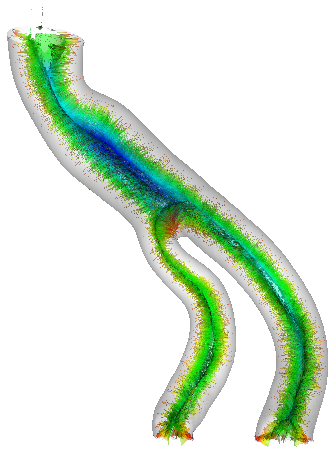
\includegraphics[width=1.5in]{Figures/overlay_100_01_voronoi_local.png}%
\label{fig:VoronoiLocal}}
\hfil
\subfloat{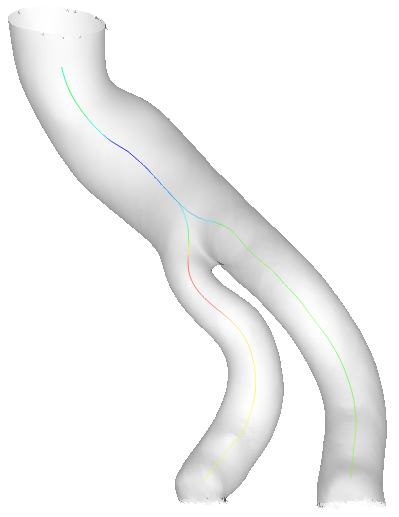
\includegraphics[width=1.5in]{Figures/overlay_100_01_centerlines_local.png}%
\label{fig:OverlayLocal}}
\caption{Centerlines extraction of the aorta in local details: (a) embedded Voronoi diagram; (b) centerlines inside the vessel.}%
\label{fig:CenterlinesLocal}
\end{figure}

\begin{figure}[t]
\centering
\subfloat{\includegraphics[height=2.0in]{Figures/overlay_100_01_voronoi.png}
%\caption{Voronoi diagrams of the abdominal aorta.}
\label{fig:VoronoiGlobal}}
\hfil
\subfloat{\includegraphics[height=2.0in]{Figures/overlay_100_01_centerlines.png}
%\caption{Centerlines of the abdominal aorta.}
\label{fig:OverlayGlobal}}
\caption{Centerlines extraction of the aorta in VOI. (a) Voronoi diagrams; (b) Centerlines. }
\label{fig:CenterlineGlobal}
\end{figure}

\subsection{Centerlines Extraction Based on Surface Model}

The centerlines extraction computation was performed on the subdivided surface model.
Firstly, the embedded Voronoi diagram of the preprocessed surface model is generated (see Fig. \ref{fig:VoronoiLocal}).
Secondly, the centerlines of the tubular surface model is computed (see Fig. \ref{fig:OverlayLocal}).
The colors marked on the Voronoi diagram and the centerlines denote the diameters of the local resection circle, decreasing from blue to red.
The same processing was straightly applied to the model surface of the whole abdominal aorta (see Fig. \ref{fig:VoronoiGlobal} and Fig. \ref{fig:OverlayGlobal}).
One can see from the details of the results that the starting and ending points are not exactly located at the ``entrances" or ``exits".
The reason of this is the Voronoi diagram on which the points consisting the centerlines exist never intersect with the model surface, i.e., the ending points of the centerlines are approaching the terminals of the surface model as near as possible, but never stick to them.
\begin{figure}[t]
\centering
\subfloat{\includegraphics[width=0.7in]{Figures/surface.png}%
\label{fig:SurfaceModel}}
\hfil
\subfloat{\includegraphics[width=0.9in]{Figures/centerlines.png}%
\label{fig:CenterlinesModel}}
\caption{Visualization models of the aorta: (a) image-based surface model (quantity of consisting polygons: $757,538$); (b) centerlines of the surface model.}%
\label{fig:VisualizationModel}
\end{figure}

\subsection{Discussions}

The computer programs used in this paper were written in C++ based on the Visualization Toolkit, an open source library aims at providing general facilities in the scientific visualization field \cite{Schroeder2000VTK}. %
To depress the unintended affections of the unstructured polygonal surfaces and the noises introduced by the image segmentation, series of steps were introduced in our experiments to extract the centerlines of the surface model of the vasculature. %
During this process, the quantities of the consisting polygons were obviously decreased for the extraction of the largest connected region in the surface model.
Due to the centerlines extraction computation is sensitive and expensive, we subdivided the smoothed surface model based on an improved butterfly scheme.
After this process, the quantities of the consisting polygonal surfaces were increased because of the refinement of the polygons.
With this step, the potential perturbation was further reduced, leading to much less errors which may occur during the computation of the centerlines extraction.
It is noteworthy that the extraction of centerlines for the model surface is an expensive computation both in time and space.
The calculation of the whole aorta (see Fig. \ref{fig:VisualizationModel}) cost nearly eight hours on our desktop machine with dedicated modification on the code to fit the bulky data into the relatively limited memory. %
%The calculation of the whole aorta cost nearly eight hours on our desktop machine with dedicated modification on the code to fit the bulky data into the relatively limited memory. %

\section{Conclusions and Future Work}
%The conclusion goes here.

Centerlines are useful in describing the shape of three dimensional objects.
In implementing the intravascular surgical simulation system, centerlines model of the vasculature will serve as the shape description for the simulation of path planning and navigation of the virtual guidewires/catheters.
In this paper, an automatic approach is designed and validated to extract the centerlines of the image-based patient-specific vasculature model.
The shape analysis presented here lays the foundation for our further research in visualizing the vessels that are closely related to the simulation of PCI procedure.

The connectivity of the polygons in the surface model is firstly checked to find out and remove the redundant polygons that are irrelevant to the actual surface.
Then the resulting surfaces are smoothed at the locations that seems to be uneven in order to prevent these perturbations against the centerlines computation.
After that, the surfaces are subdivided by applying an improved butterfly scheme with the aim of acquiring a more precise surface model.
Finally, the Eikonal equation of the time of arrivals of the embedded Voronoi diagram is computed to obtain the centerlines of the model surface.
Experiments are designed and carried out with the results in demonstrating the effectiveness of the developed approach.

In the future, our research directions are further optimization of the surface model on the one hand, and the visualization of other organs (e.g., heart) and the simulation of the typical phenomena (such as contrast injection, heart beat, etc.) during the procedure on the other. %

%# -*- coding:utf-8 -*-
\chapter{躯干部解剖环境的构建}
\label{chap6}

本章叙述内容:
\begin{enumerate}
  \item 引言
  \item X光影效果
  \item 造影剂注入效果
  \item 心脏搏动效果
  \item 实际验证
  \item 本章小结
\end{enumerate}

\section{引言}

\section{X光影效果}
\label{sec6.2}

\section{造影剂注入效果}

\section{心脏搏动效果}

\section{实际验证}

\section{本章小结}
%# -*- coding:utf-8 -*-
\chapter{组织的物理特性建模及其与手术工具的交互}
\label{chap7}

难点,并且用基于模型的策略来解决姿态评价和
优化的方法往往会具有更好的性能。这里我们以交通场景为研究背景,
讨论基于交通路面场景的运动检测、车辆定位、摄像机标定和模型可. 
%# -*- coding:utf-8 -*-
\chapter{手术流程的状态机模型研究}
\label{chap8}

一般地,一个跟踪预测滤波器的滤波结果好坏取决于两方面的因素:运动模型和滤波器的结构。

本章中提出了一种新的车辆运动模型。
在这个运动模型中考虑了车辆行驶过程中的运动学特性,从而比以前的运动模型更符
合车辆的真实运动。现有的车辆跟踪系统中大多使用了扩展卡尔曼滤波器或者其各种变
体,但是在车辆运动比较复杂时效果不是很好。本章使用了一种改进的扩展卡尔曼滤波器,
加入了一个新的优化目标。实验结果表明,在跟踪车辆运动时,本文中的方法有一定的优点。 
%# -*- coding:utf-8 -*-
\chapter{软件系统的整合}
\label{chap9}

本章叙述内容:
\begin{enumerate}
  \item 引言
  \item 软件系统的设计
  \item 相关的软件库
  \item 工程注记
  \item 本章小结
\end{enumerate}

\section{引言}

\section{软件系统的设计}

\section{相关的软件库}

\section{工程注记}

\section{本章小结}
%# -*- coding:utf-8 -*-
\chapter{总结与展望}
\label{chap10}

自从Marr在其1982年的著名论著\cite{Marr:1982}中提出计算机视觉的理
论框架以来,世界上掀起了研究计算机视觉的高潮,研究者们针对视觉的有关
问题进行了大量的工作,并取得了很大进展。但是,传统的计算机视觉研究
常常认为视觉感知过程的主要任务是物体的三维重建,例如Marr提出的一般
化圆柱模型(generalized
cylinders)\cite{Marr:1982}。从而,二十世纪八九十年代大量关于图像
序列的研究工作主要集中在恢复场景的三维几何结构(如structure from
motion),计算摄像机的运动(ego-motion)和象素的运动信息(例如 光流计算optical
flow)等,很少涉及到图像的高层语义信息。近几年来,对图像序列中的运动
理解越来越受到国际学术界的重视,甚至有人预测动态图像
序列分析和理解将成为21世纪计算机视觉的研究重点。

本文针对路面交通场景动态图像序列的语义理解进行了深入研究,涉及到许多
动态图像语义理解的基本问题,包括摄像机标定、运动检测和分割、目标定位和识别、时空推理、
场景恢复与表示、行为分析和建模、语义理解等等。 


% 附录
\begin{appendix}
\renewcommand{\chaptername}{附录 \Alph{chapter}}
%# -*- coding:utf-8 -*-
\chapter{软件系统的整合}
\label{chap1a}

本章叙述内容:
\begin{enumerate}
  \item 引言
  \item 软件系统的设计
  \item 相关的软件库
  \item 工程注记
  \item 本章小结
\end{enumerate}

\section{引言}

\section{软件系统的设计}

\section{相关的软件库}

\section{工程注记}

\section{本章小结} 
%# -*- coding:utf-8 -*-
\chapter{软件系统的整合}
\label{chap1a}

本章叙述内容:
\begin{enumerate}
  \item 引言
  \item 软件系统的设计
  \item 相关的软件库
  \item 工程注记
  \item 本章小结
\end{enumerate}

\section{引言}

\section{软件系统的设计}

\section{相关的软件库}

\section{工程注记}

\section{本章小结} 
\end{appendix}
\backmatter %结束章节自动编号

%参考文献
\cleardoublepage
\phantomsection
\bibliographystyle{thubib}
%\bibliographystyle{unsrt}
\addcontentsline{toc}{chapter}{参考文献}
\addtolength{\bibsep}{-4.5pt} % 缩小参考文献间的垂直间距
\bibliography{Reference/myreference_UTF8}

%\frontmatter
%攻读博士学位期间的研究成果
%# -*- coding:utf-8 -*- 
%=========================================================================%
%   LaTeX File for phd thesis of Institute of Automation, CAS
%-------------------------------------------------------------------------%
%   Revised by J. G. Lou (jglou@nlpr.ia.ac.cn)
%-------------------------------------------------------------------------%
%%%%%%%%%%%%%%%%%%%%%%%%%%%%%%%%%%%%%%%%%%%%%%%%%%%%%%%%%%%%%%%%%%%%%%%%%

\chapter*{攻读博士期间发表的论文\markboth{攻读博士学位期间发表的论文}{攻读博士学位期间发表的论文}}
\addcontentsline{toc}{chapter}{攻读博士学位期间发表的论文}
\begin{enumerate}
   \item[1.] \textbf{Fan Yang}, Zeng-Guang Hou, Shao-Hua Mi, Gui-Bin Bian and Xiao-Liang Xie, "3D Modeling of Coronary Arteries Based on Tubular-Enhanced CURVES Segmented Regions for Robotic Surgical Simulation", 2013 International Conference (IEEE-ROBIO 2013) on Robotics and Biomimetics, 12th December 2013.
%   \item[2.] \textbf{楼建光},柳崎峰,胡卫明,谭铁牛, "交通视觉监控中的摄像机参数求解", 计算机学报, 第25卷, 第11册, 2002年11月.
%   \item[3.] \textbf{Jianguang Lou}, Qifeng Liu, Tieniu Tan and Weiming Hu, "Semantic interpretation of object activities in a surveillance system", IEEE International Conference on Pattern Recognition, Canada, 2002 (\textbf{oral presentation}).
%   \item[4.] \textbf{Jianguang Lou}, Hao Yang, Weiming Hu, Tieniu Tan, "Visual Vehicle Tracking Using An Improved EKF", the 5th Asia Conference on Computer Vision, Australia, 2002 (\textbf{oral presentation}).
%   \item[5.] \textbf{Jianguang Lou}, Hao Yang, Weiming Hu, Tieniu Tan, "An Illumination Invariant Change Detection Algorithm", the 5th Asia Conference on Computer Vision, Australia, 2002 (\textbf{oral presentation}).
%   \item[6.] Hao Yang, \textbf{Jianguang Lou}, Hongzan Sun, Weiming Hu and Tieniu Tan, "Efficient and robust vehicle localization", Proceeding of IEEE International Conference on Image Processing, Vol.2, pp. 355-358, Greece, 2001.
%   \item[7.] Qifeng Liu, \textbf{Jianguang Lou}, Weiming Hu, Tieniu Tan, "Comparison of model-based pose evaluation algorithm in traffic scenes", the 2nd International Conference on Image and Graphics, Hefei, 2002.
%   \item[8.] 柳崎峰,\textbf{楼建光},"智能视觉监控技术",科学新闻,第23期,pp. 35-36, 2002年12月.
\end{enumerate}



% 致谢
%# -*- coding:utf-8 -*- 
%=========================================================================%
%   LaTeX File for phd thesis of Institute of Automation, CAS
%-------------------------------------------------------------------------%
%   Revised by J. G. Lou (jglou@nlpr.ia.ac.cn)
%-------------------------------------------------------------------------%
%%%%%%%%%%%%%%%%%%%%%%%%%%%%%%%%%%%%%%%%%%%%%%%%%%%%%%%%%%%%%%%%%%%%%%%%%

\chapter*{致\ 谢\markboth{致\ 谢}{致\ 谢}}
\addcontentsline{toc}{chapter}{致谢}



值此学位论文完成之际,我要向我的导师侯增广研究员表示最衷心感谢。老师渊博的学识,
对学术发展的敏锐眼光,对科研事业的执着追求和对工作的热忱,以及对我们研究生的关
心和爱护,都深深地鼓舞和影响了我。所有这些,都令学生受益终生!

感谢复杂系统管理与控制国家重点实验室机器人研究组的各位老师为我们营造的这样一个
良好的学习环境。感谢同组已毕业的同学吉程博士和徐飞硕士,与他们的讨论激发了我的
创意和兴趣;感谢同组同届的同学米韶华和陈翼雄,这共同攻读博士学位的“苦难岁月”
让我们成为了战友;感谢同组的其他同学对我的帮助和支持。同机器人研究组的导师和同
学一起学习和工作的时光,将是我个人学习生涯中最难以忘怀的。

感谢上海市胸科医院的方唯一教授和曲新凯博士,感谢他们在百忙中抽出宝贵的时间为我
们耐心地讲解和演示经皮介入冠状动脉导管术,热心回复我们在工作中遇到的医学方面的
问题,并为我们提供了宝贵的医学资料。

感谢开源软件社区的每一位黑客,感谢他们在智慧上的无私分享。如果没有这些设计优雅、
性能优异的专业级别的开源软件工具,那么我们的研究工作很可能无法在这短短几年中完
成。

感谢中国科学院自动化研究所研究生部的各位工作人员为我在研究所学习和工作期间提供
的咨询和帮助。

最深的感谢送给我的父母,感谢他们孜孜不倦的教诲和无限的宽容与鼓励。感谢我的妹妹,
家庭的开心果,感谢与她共同成长成人的岁月,感谢她带给我们的每一次开怀大笑。最后,
我要感谢我的妻子,感谢她给我无尽的爱和支持。
\\
\\
\\
\\
\hspace*{10.8cm}2013年10月


\clearpage
\end{CJK*}
\end{document}
%%%%%%%%%%%%%%%%%% End of the file  %%%%%%%%%%%%%%%%%%%%%%%%

\bibliography{Reference/myreference_UTF8}
%\bibliography{mythesis_UTF8}

%\frontmatter
%攻读博士学位期间的研究成果
%# -*- coding:utf-8 -*- 
%=========================================================================%
%   LaTeX File for phd thesis of Institute of Automation, CAS
%-------------------------------------------------------------------------%
%   Revised by J. G. Lou (jglou@nlpr.ia.ac.cn)
%-------------------------------------------------------------------------%
%%%%%%%%%%%%%%%%%%%%%%%%%%%%%%%%%%%%%%%%%%%%%%%%%%%%%%%%%%%%%%%%%%%%%%%%%

\chapter*{攻读博士期间发表的论文\markboth{攻读博士学位期间发表的论文}{攻读博士学位期间发表的论文}}
\addcontentsline{toc}{chapter}{攻读博士学位期间发表的论文}
\begin{enumerate}
   \item[1.] \textbf{Fan Yang}, Zeng-Guang Hou, Shao-Hua Mi, Gui-Bin Bian and Xiao-Liang Xie, "3D Modeling of Coronary Arteries Based on Tubular-Enhanced CURVES Segmented Regions for Robotic Surgical Simulation", 2013 International Conference (IEEE-ROBIO 2013) on Robotics and Biomimetics, 12th December 2013.
%   \item[2.] \textbf{楼建光},柳崎峰,胡卫明,谭铁牛, "交通视觉监控中的摄像机参数求解", 计算机学报, 第25卷, 第11册, 2002年11月.
%   \item[3.] \textbf{Jianguang Lou}, Qifeng Liu, Tieniu Tan and Weiming Hu, "Semantic interpretation of object activities in a surveillance system", IEEE International Conference on Pattern Recognition, Canada, 2002 (\textbf{oral presentation}).
%   \item[4.] \textbf{Jianguang Lou}, Hao Yang, Weiming Hu, Tieniu Tan, "Visual Vehicle Tracking Using An Improved EKF", the 5th Asia Conference on Computer Vision, Australia, 2002 (\textbf{oral presentation}).
%   \item[5.] \textbf{Jianguang Lou}, Hao Yang, Weiming Hu, Tieniu Tan, "An Illumination Invariant Change Detection Algorithm", the 5th Asia Conference on Computer Vision, Australia, 2002 (\textbf{oral presentation}).
%   \item[6.] Hao Yang, \textbf{Jianguang Lou}, Hongzan Sun, Weiming Hu and Tieniu Tan, "Efficient and robust vehicle localization", Proceeding of IEEE International Conference on Image Processing, Vol.2, pp. 355-358, Greece, 2001.
%   \item[7.] Qifeng Liu, \textbf{Jianguang Lou}, Weiming Hu, Tieniu Tan, "Comparison of model-based pose evaluation algorithm in traffic scenes", the 2nd International Conference on Image and Graphics, Hefei, 2002.
%   \item[8.] 柳崎峰,\textbf{楼建光},"智能视觉监控技术",科学新闻,第23期,pp. 35-36, 2002年12月.
\end{enumerate}



% 致谢
%# -*- coding:utf-8 -*- 
%=========================================================================%
%   LaTeX File for phd thesis of Institute of Automation, CAS
%-------------------------------------------------------------------------%
%   Revised by J. G. Lou (jglou@nlpr.ia.ac.cn)
%-------------------------------------------------------------------------%
%%%%%%%%%%%%%%%%%%%%%%%%%%%%%%%%%%%%%%%%%%%%%%%%%%%%%%%%%%%%%%%%%%%%%%%%%

\chapter*{致\ 谢\markboth{致\ 谢}{致\ 谢}}
\addcontentsline{toc}{chapter}{致谢}



值此学位论文完成之际,我要向我的导师侯增广研究员表示最衷心感谢。老师渊博的学识,
对学术发展的敏锐眼光,对科研事业的执着追求和对工作的热忱,以及对我们研究生的关
心和爱护,都深深地鼓舞和影响了我。所有这些,都令学生受益终生!

感谢复杂系统管理与控制国家重点实验室机器人研究组的各位老师为我们营造的这样一个
良好的学习环境。感谢同组已毕业的同学吉程博士和徐飞硕士,与他们的讨论激发了我的
创意和兴趣;感谢同组同届的同学米韶华和陈翼雄,这共同攻读博士学位的“苦难岁月”
让我们成为了战友;感谢同组的其他同学对我的帮助和支持。同机器人研究组的导师和同
学一起学习和工作的时光,将是我个人学习生涯中最难以忘怀的。

感谢上海市胸科医院的方唯一教授和曲新凯博士,感谢他们在百忙中抽出宝贵的时间为我
们耐心地讲解和演示经皮介入冠状动脉导管术,热心回复我们在工作中遇到的医学方面的
问题,并为我们提供了宝贵的医学资料。

感谢开源软件社区的每一位黑客,感谢他们在智慧上的无私分享。如果没有这些设计优雅、
性能优异的专业级别的开源软件工具,那么我们的研究工作很可能无法在这短短几年中完
成。

感谢中国科学院自动化研究所研究生部的各位工作人员为我在研究所学习和工作期间提供
的咨询和帮助。

最深的感谢送给我的父母,感谢他们孜孜不倦的教诲和无限的宽容与鼓励。感谢我的妹妹,
家庭的开心果,感谢与她共同成长成人的岁月,感谢她带给我们的每一次开怀大笑。最后,
我要感谢我的妻子,感谢她给我无尽的爱和支持。
\\
\\
\\
\\
\hspace*{10.8cm}2013年10月


\clearpage
\end{CJK*}
\end{document}
%%%%%%%%%%%%%%%%%% End of the file  %%%%%%%%%%%%%%%%%%%%%%%%
